\documentclass[msc]{mestrado}
 
\usepackage{master}

%% Inicio do documento
\begin{document}
\mainmatter

\headsep=20pt
\oddsidemargin=14pt

\setstretch{1.4}
\parskip=3pt

%\chapter{Introdu��o}

%\chapter{Ethernet e Tempo Real}
\label{cap:motivacao}

%\chapter{O Protocolo \doris{}} % (10 pag)
\label{cap:doris}

%\chapter{A disciplina \emph{DoRiS}} % (10 pag)
\label{cap:specVerif}

%\chapter{Plataforma Operacional}
\label{cap:platOp}

\chapter{Plataforma Operacional}
\label{cap:platOp}

\section{Introdu��o}
\label{sec:introPlatOp}

Nos cap�tulos que precedem, o protocolo \doris{} foi descrito e os seus objetivos
foram apresentados.  Depois desta fase de defini��o, especifica��o formal e
valida��o do protocolo \doris{}, � chegado o momento de apresentar um outro desafio
deste projeto de desenvolvimento de um protocolo de comunica��o de tempo real
baseado em Ethernet. Isto �, a escolha de uma plataforma operacional de tempo real
h�brida, de c�digo livre, que possa ser utilizada tanto em computadores de uso geral
quanto em dispositivos dedicados e que atende aos requisitos temporais necess�rios
para a implementa��o do protocolo \doris{}.

� importante notar aqui que o desafio principal concentra-se em torno do uso dos
computadores de uso geral. De fato, os dispositivos dedicados utilizam sistemas
embarcados ou micro-controladores para oferecer um conjunto de funcionalidades
definidas. Integrar tais dispositivos num sistema distribu�do requer levar em conta
as suas restri��es espec�ficas como, por exemplo, capacidade de processamento, taxa
de transfer�ncia, consumo de energia, etc. No entanto, a qualidade dos servi�os
oferecidos por tais dispositivos � uma conseq��ncia do seu
projeto. Conseq�entemente, uma vez especificados os requisitos do sistema, o
dispositivo pode ser escolhido adequadamente de tal forma a satisfazer estes
requisitos.

No caso dos computadores de uso geral, a situa��o � bastante diferente, pois o
primeiro objetivo a ser alcan�ado � o desempenho geral do sistema. No entanto, as
tecnologias modernas utilizadas nas arquiteturas de computadores atuais para
aumentar o desempenho dos dispositivos de hardware s�o muitas vezes fontes de
imprevisibilidade temporal.  Isto �, por exemplo, o caso da mem�ria \ing{cache}, do
acesso direto � mem�ria (DMA), do co-processamento, da predi��o de instru��es, das
unidades \ing{multicore} ou dos \ing{pipelines}.  Devem tamb�m ser mencionadas as
fun��es de gerenciamento da energia, que, por afetar a freq��ncia de execu��o do
processador, dificultam a estimativa dos piores casos dos tempos de execu��o dos
programas. Tal complexidade do hardware, embora torne os sistemas computacionais
mais velozes, aumenta o grau de imprevisibilidade do sistema e dificulta a
estimativa dos atributos necess�rios � teoria do escalonamento de Sistemas de Tempo
Real \cite{Liu73, Audsley93, Tindell94}.  No entanto, reduzir o conjunto de servi�os
oferecidos por um Sistema Operacional de Prop�sito Geral (SOPG) no patamar dos SOs
que podem garantir previsibilidade equivale a negar as evolu��es do hardware das
�ltimas d�cadas.  Para resolver este desafio, v�rias abordagens foram propostas ao
longo do tempo para desenvolver plataformas operacionais determin�sticas baseadas em
SOPG.

Este cap�tulo apresenta algumas destas abordagens com o objetivo de escolher a
plataforma operacional que oferecer� suporte � implementa��o de \doris. Como esta
dever� ser de software livre, usar a fam�lia de sistemas Linux parece ser uma
tend�ncia natural. Inicialmente, uma explica��o geral sobre as principais
caracter�sticas de Linux � apresentada na se��o \ref{sec:LinuxSOPG}. Como ser�
visto, Linux oferece v�rios aspectos que impedem seu uso direto na implementa��o de
\doris. Tais aspectos ser�o detalhados na se��o \ref{sec:compTemp}. Em seguida,
algumas das tend�ncias que t�m incorporado caracter�sticas de sistemas de tempo real
em Linux ser�o descritas na se��o \ref{sec:sotrLinux}. Por fim, resultados
comparativos de algumas plataformas ser�o apresentados na se��o
\ref{sec:experimentos} e a escolha de uma destas ser� justificada, de acordo com as
necessidade de \doris.


\section{Linux: um Sistema Operacional de Prop�sito Geral}
\label{sec:LinuxSOPG}

Depois de uma breve justificativa da escolha do Linux para este trabalho, esta se��o
apresenta os principais elementos do sistema Linux que causam ou que s�o
relacionados � exist�ncia de imprevisibilidade temporal na execu��o das
aplica��es.

\subsection{Motiva��o para o uso de Linux}
\label{sec:porque}

A escolha da plataforma operacional no contexto deste trabalho se deu pelas
caracter�sticas do protocolo \doriss e pelo contexto universit�rio do seu
desenvolvimento. Resumidamente, os seguintes crit�rios foram adotados
para determinar uma plataforma adequada para desenvolvimento de \doris:

\begin{enumerate}
\item ser de c�digo livre e aberto (licen�a GPL);
\item garantir desvios m�ximos da ordem da dezena de micro-segundos para as
  aplica��es de controle via rede, conforme o padr�o de qualidade de servi�o
  oferecida pelos Sistemas Operacionais de Tempo Real (SOTR);
\item permitir o uso de aplica��es multim�dia, banco de dados e outros componentes
  de software distribu�dos tipicamente usadas em ambientes multi-usu�rios de
  Sistemas Operacionais de Prop�sito Geral (SOPG);
\item prover suporte �s aplica��es embarcadas usando componentes de prateleira.
\end{enumerate}

A primeira destas condi��es decorre do modelo de pesquisa e desenvolvimento
defendido neste trabalho. Apesar de a ecologia pol�tica ser um assunto
essencial aos olhos deste mesmo, foge do escopo deste trabalho apresentar os
elementos referindo a este t�pico.  A leitura de Andr� Gorz \cite{Gorz77} ou Milton
Santos \cite{Santos00} dever� saciar a curiosidade dos mais interessados.

A segunda condi��o decorre dos requisitos temporais das aplica��es de controle e
corresponde tamb�m �s margens de desvios necess�rias para a implementa��o do
protocolo \doris, conforme visto no cap�tulo \ref{cap:doris}. Finalmente, o terceiro
e quarto itens s�o diretamente relacionados com as metas do protocolo \doris, que j�
foram amplamente discutidas nos cap�tulos~\ref{cap:motivacao}~e~\ref{cap:doris}.

Dentre as solu��es de SOPG, o sistema Linux \cite{Kernel, Bovet05} � um software
livre e de c�digo aberto que se distingue pela originalidade da sua proposta de
desenvolvimento sob licen�a GNU/GPL (GNU \ing{General Public License}).  Uma
conseq��ncia direta deste modelo de desenvolvimento cooperativo � que o \kernell
Linux conta com uma das maior comunidade de desenvolvedores espalhada pelo mundo
inteiro. Outra vantagem do \kernell Linux � ser baseado no sistema UNIX e oferecer
uma interface de utiliza��o conforme o padr�o POSIX \ing{Portable Operating System
  Interface} \cite{POSIX04}. Por fim, deve ser observado que Linux � bastante
difundido nos ambientes de pesquisa acad�mica.

Por todas estas raz�es, a plataforma Linux apareceu como uma candidata pertinente para
este projeto de pesquisa. No entanto, como ser� visto mais adiante, o \kernell Linux
por si s� n�o oferece as garantias temporais definidas no item (iv) acima. Portanto,
revelou-se necess�rio pesquisar solu��es existentes para tornar o SOPG Linux
determinista. Algumas destas solu��es s�o apresentadas ao longo deste cap�tulo,
assim como a extens�o Linux de tempo real adotada no contexto deste trabalho.

% Observa-se que nos sistemas de tempo real, o desempenho � um objetivo secund�rio,
% subordinado ao determinismo.  Esta constata��o e as facilidades que trazem a
% possibilidade de trabalhar no ambiente de programa��o Linux t�m levado v�rios grupos
% de pesquisa a utilizar a plataforma Linux para fins de pesquisa sobre SOTR. Num
% trabalho recente, por exemplo, Linux esta sendo utilizado para desenvolver a
% plataforma $LITMUS^{RT}$ para testar algoritmos de escalonamento para arquiteturas
% multiprocessadas \cite{Calandrino06}.

Antes de abordar a caracteriza��o das propriedades temporais do Linux e de algumas
de suas extens�es de tempo real, s�o apresentados brevemente alguns conceitos
b�sicos de sistemas operacionais que s�o utilizados intensivamente ao longo deste
cap�tulo.

\subsection{Interrup��es }
\label{sec:interrupt}

Na classe do sistema do tipo UNIX \cite{Bach86}, na qual se encontra o sistema
Linux, o SO, ou simplesmente, \kernel, executa num modo diferente
dos demais processos: o modo ``protegido''. Diz-se que os processos,
associados �s aplica��es, executam em modo ``usu�rio''. Estes dois modos s�o
definidos no n�vel do hardware do processador e s�o utilizados para restringir o
acesso aos dispositivos de hardware da m�quina. Por este meio, garante-se que os
�nicos processos que podem obter acesso aos dispositivos de hardware s�o aqueles
executando em modo protegido.  Respons�vel pelo gerenciamento dos recursos, o
\kernell prov� uma camada de abstra��o dos dispositivos de hardware aos processos
usu�rios. A interface do Linux � oferecida atrav�s de trechos de c�digo
denominados ``chamadas de sistema''. Cada uma destas chamadas oferece uma API (Interface de
Programa��o da Aplica��o) padronizada pela norma POSIX \cite{POSIX04},  para
facilitar tanto o trabalho dos programadores, quanto a portabilidade dos c�digos de
software.

A organiza��o da comunica��o entre os dispositivos, o \kernell e as aplica��es �
baseada no conceito de interrup��o do processador. Tais interrup��es s�o gerenciadas
por um dispositivo de hardware espec�fico, o PIC ou o APIC (\ing{Advanced
  Programmable Interrupt Controller}) que � diretamente conectado ao processador.
Na ocorr�ncia de um evento de comunica��o, ou seja, quando um dispositivo requer a
aten��o do processador, ele informa ao APIC via uma linha de interrup��o (\ing{IRQ lines}).
 Por sua vez, o APIC informa ao processador que uma interrup��o precisa ser tratada.

 Distinguem-se as interrup��es s�ncronas e ass�ncronas. As primeiras s�o geradas pelo
 pr�prio processo em execu��o no final do ciclo de execu��o de uma instru��o.  Elas
 correspondem ao uso de instru��es espec�ficas pelo programa, tais como as chamadas
 de sistema da interface do \kernel, ou podem ser causadas pela execu��o de uma
 instru��o indevida.  As interrup��es ass�ncronas s�o geradas pelos dispositivos de
 hardware para informar ao processador a ocorr�ncia de um evento externo e podem ser
 geradas a qualquer instante do ciclo do processador.

 Quando o processador percebe uma interrup��o, quer seja s�ncrona ou ass�ncrona, ele
 desvia sua execu��o e passa a executar o tratador de interrup��o associado � linha
 de interrup��o que solicitou o APIC inicialmente.  Esta execu��o n�o � associada a
 processo algum, mas sim � ocorr�ncia de um evento e, portanto, n�o tem contexto de
 execu��o pr�prio.  O tratador simplesmente executa no contexto do �ltimo processo
 que estava executando no processador.

 Para minimizar o impacto das interrup��es sobre a execu��o dos processos regulares,
 um tratador de interrup��o � geralmente subdividido em tr�s partes. A primeira
 parte executa opera��es cr�ticas que n�o podem ser atrasadas e que modificam
 estruturas de dados compartilhadas pelo dispositivo e o \kernel.  Tais opera��es
 s�o executadas imediatamente e com as interrup��es desabilitadas. Tamb�m executado
 imediatamente pelo tratador, mas com as interrup��es habilitadas, s�o as opera��es
 r�pidas que modificam apenas as estruturas de dados do \kernel, pois estas s�o
 protegidas por mecanismos de \ing{locks}, assim como ser� vista na se��o
 \ref{sec:locks}.  Estes dois conjuntos de opera��es constituem a parte cr�tica do
 tratador, durante a qual a execu��o n�o pode ser suspensa.  Finalmente, as
 opera��es n�o-cr�ticas e n�o-urgentes s�o possivelmente adiadas e executadas com as
 interrup��es habilitadas. Estas execu��es s�o chamadas de \cod{softirqs} ou
 \cod{tasklets}.

Do tratamento eficiente das interrup��es depende a capacidade do sistema para reagir a
eventos externos. O \kernell padr�o garante esta efici�ncia, proibindo que a execu��o
da parte cr�tica do tratador de interrup��o seja suspensa, mas permitindo que a
parte n�o-cr�tica, e geralmente mais demorada, seja suspensa para a execu��o da
parte cr�tica de uma outra interrup��o.

\subsection{Tempo compartilhado}
\label{sec:tick}

O principal objetivo de um Sistemas Operacional de Prop�sito Geral (SOPG), tal como
Linux, � oferecer o melhor servi�o poss�vel para o uso compartilhado por v�rios
usu�rios de recursos limitados, tal como processadores, mem�ria, disco, placas de
rede e outros dispositivos de \ing{hardware} \cite{Bach86, Tanenbaum01, Oliveira01}.
Um usu�rio do sistema, compartilhando um conjunto de recursos, dever� ter
a ilus�o que est� sozinho atuando naquele sistema. O SOPG deve, portanto,
garantir o acesso dos usu�rios a todos os recursos que ele gerencia com lat�ncias
impercept�veis para um ser humano. A implementa��o de tal servi�o, cuja qualidade
depende altamente da subjetividade de cada usu�rio e das aplica��es que ele precisa
executar, utiliza o mecanismo de compartilhamento temporal dos recursos. Para dar a
impress�o de exclusividade e continuidade dos servi�os aos usu�rios, os recursos s�o
alocadas sucessivamente �s aplica��es por fatias de tempos curtas, da ordem de
alguns milisegundos. A altern�ncia r�pida destas aloca��es garante que cada
aplica��o ganhe o acesso ao recurso com uma freq��ncia suficiente para que n�o haja
tempo ocioso percept�vel do ponto de visto do usu�rio. O modelo de tempo compartilhado
caracteriza assim os sistemas multi-program�veis e multi-usu�rios.

No Linux e em SOPG similares, o entrela�amento das execu��es dos processos ao longo
do tempo � realizado da seguinte maneira.  O tempo � dividido em intervalos de
tamanho iguais. Para este efeito, o SO utiliza o PIT (\ing{Programable Interrupt
  Timer}), baseado, nas arquiteturas PCs i386, num de hardware dedicado - o chip
8254 ou seu equivalente.  O PIT � programado para gerar uma interrup��o peri�dica, o
\ing{tick}, cujo per�odo, chamado de $jiffy$, � configur�vel, variando entre $1$ e
$10\mu s$ em fun��o das arquiteturas. 

A cada \ing{tick} uma interrup��o ocorre. Esta provoca a atualiza��o e execu��o
eventual dos temporizadores do sistema assim como a chamada do escalonador quando
isto se faz necess�rio. Conseq�entemente, quanto menor o $jiffy$, mais freq�entes
ser�o as ativa��es de cada processo, melhorando assim a capacidade de rea��o do
sistema.  Por outro lado, com um $jiffy$ pequeno, a altern�ncia entre os processos �
mais freq�ente, aumentando o tempo gasto em modo \kernel, no qual o processador s�
executa tarefas de gerenciamento.  Portanto, escolher a freq��ncia dos \ing{ticks}
constitui um compromisso entre o desempenho do sistema e a resolu��o desejada para
escalonar os processos.  Observa-se, em particular, que a implementa��o do tempo
compartilhado por \ing{ticks} de dura��o constante faz com que um processo n�o possa
``dormir'' por um tempo menor do que um \ing{jiffy}.

Al�m disso, o algoritmo de gerenciamento dos temporizadores, chamado de ``roda dos
temporizadores'', pode constituir uma outra fonte de sobrecarga nos sistemas que
utilizam muitos temporizadores. Este algoritmo utiliza uma estrutura de
armazenamento baseada em 5 faixas de $jiffies$ correspondendo a intervalos de tempo
que crescem exponencialmente \cite{Bovet05, Molnar05}. Cada faixa armazena os
temporizadores de acordo com os seus valores de instantes de expira��o. A primeira
faixa corresponde aos temporizadores com tempos de expira��o contidos no intervalo
indo de $1$ a $256 \, jiffies$. A segunda corresponde aos temporizadores expirando
entre $257 \, jiffies$ e $16384 \, jiffies$ e assim por diante at� a quinta faixa
que corresponde a todos os temporizadores expirando depois de $67108865 \,
jiffies$. Quando um temporizador � criado, ele � armazenado na faixa que cont�m o
$jiffy$ no qual ele deve expirar. A cada $256$ $jiffies$, depois que todos os
temporizadores da primeira faixa sejam eventualmente disparados, o sistema executa a
rotina chamada ``cachoeira'' que atualiza as diferentes faixas, cascateando os
temporizadores de faixa em faixa.  Por exemplo, esta rotina determina quais s�o os
temporizadores da segunda faixa que v�o expirar nos pr�ximos $256$ $jiffies$ e os
transferem para a primeira faixa. Similarmente, a rotina transfere os devidos
temporizadores da terceira para a segunda faixa, da quarta para terceira e da quinta
para a quarta.

Al�m de utilizar uma estrutura de dados de tamanho limitado, este algoritmo se torna
muito eficiente quando os temporizadores s�o apagados antes de serem disparados. Isto
ocorre, por exemplo, no caso de uma esta��o servidor Internet na qual a grande
maioria dos temporizadores s�o cancelados rapidamente. Neste caso, a sobrecarga
causada pela execu��o da rotina da cachoeira passa a ser insignificante, pois os
temporizadores s�o cancelados antes de serem cascateados. Por outro lado, percebe-se
que a diminui��o da dura��o do $jiffy$ aumenta a sobrecarga gerada por este
algoritmo, pois a rotina da ``cachoeira'' acaba sendo executada mais
freq�entemente. Al�m disso, sendo o tempo entre cada execu��o menor, o n�mero de
temporizadores ainda n�o cancelados � maior. Conseq�entemente, o n�mero de
transfer�ncias de faixa a ser realizado para cada temporizador, antes do seu
cancelamento eventual, aumenta.

Na sua publica��o inicial, o \kernell 2.6 passou a usar um $jiffy$ de
$1ms$. Percebeu-se ent�o que este valor gerou uma sobrecarga significativa no
sistema, notadamente devido aos temporizadores utilizados pelas conex�es TCP. Este
fato explica em parte porque as vers�es do \kernell  posteriores a 2.6.13 v�m com o
valor padr�o do $jiffy$ de $4 ms$, e n�o mais de $1 ms$.


\subsection{Preemp��o}

No contexto dos escalonadores baseados em prioridade, um processo de baixa
prioridade pode ser suspenso no decorrer da sua execu��o para ceder o processador a
uma processo de prioridade mais alta. Quando tal evento ocorre, diz-se que houve
preemp��o do processo em execu��o pelo processo de mais alta prioridade.  De forma
geral, diz-se que houve preemp��o de um processo A por um processo B, quando o
processo A deve interromper sua execu��o para ceder o processador ao processo B. No
caso dos processos executando em modo usu�rio, a preemp��o corresponde � altern�ncia
de processos que o \kernell executa para a implementa��o do mecanismo de tempo
compartilhado.  Este procedimento se torna mais complexo quando se trata da
preemp��o de processos executando em modo \kernel.

Diz-se, de maneira simplificada, que o \kernell � preemptivo se uma altern�ncia de
processos pode acontecer quando o processador est� em modo protegido. Considere, por
exemplo, um processo A executando um tratador de exce��o associado a uma chamada de
sistema.  Enquanto A est� executando, o tratador de uma interrup��o de hardware
acorda um processo B mais priorit�rio que A. Num \kernell n�o preemptivo, o \kernell
completa a execu��o da chamada de sistema de A antes de entregar o processador para
o processo B. No caso de um \kernell preemptivo, o \kernell suspende
a execu��o da chamada de sistema para come�ar a executar B imediatamente.  Eventualmente,
depois da execu��o de B, o processo A ser� escalonado novamente e a chamada de
sistema poder� ser finalizada.

O principal objetivo de tornar o SO preemptivo \cite{Bovet05} � diminuir o tempo de
lat�ncia que o processo de mais alta prioridade pode sofrer antes de ganhar o
processador. Este objetivo � de suma import�ncia para que um SOPG
tal como Linux possa oferecer as garantias temporais encontradas em STR.


\subsubsection{Concorr�ncia e sincroniza��o}
\label{sec:locks}

Um dos desafios em tornar o \kernell preemptivo � garantir a integridade dos dados,
mesmo que v�rios caminhos de controle do \kernell possam ter acesso aos mesmos dados
de forma concorrente. Este � um problema fundamental e � comumente conhecido como
problema da exclus�o m�tua \cite{Dijkstra65, Lamport74, Raynal86, Mellor91,
  Lamport05}.  No entanto, j� que as solu��es adotadas pelo \kernell fazem parte
das principais causas de imprevisibilidade temporal do Linux padr�o, vale a pena
apresentar brevemente estas solu��es.

Chama-se de regi�o cr�tica qualquer recurso ou estrutura de dados que s� pode ser
utilizado por um processo (ou um conjunto de processos) de forma at�mica. Isto �, se
um processo $P$ entra numa regi�o cr�tica, nenhum outro processo pode entrar nesta
mesma regi�o cr�tica enquanto $P$ n�o a liberou.  Uma maneira simples de garantir a
exclus�o m�tua num sistema monoprocessado � desabilitar a possibilidade de preemp��o
durante a execu��o de uma regi�o cr�tica. Esta solu��o, bastante utilizada nas
vers�es do \kernell n�o superiores � vers�o 2.4, tem dois inconvenientes
relevantes. Primeiro, ela s� funciona em sistemas monoprocessados e, segundo, ela
n�o impede o acesso da regi�o cr�tica por tratadores de interrup��o. Neste segundo
caso, para garantir a exclus�o m�tua, um processo entrando numa regi�o cr�tica que �
compartilhada com tratadores de interrup��es deve tamb�m desabilitar aquelas
interrup��es.

Nas suas vers�es mais recentes, a partir da vers�o 2.6, o \kernell tenta reduzir ao m�ximo o
uso de tais solu��es, que comprometem o desempenho do sistema em termos de capacidade
reativa. No entanto, existem situa��es nas quais o uso destes mecanismos �
necess�rio.  Para este efeito, a implementa��o da exclus�o m�tua em contextos
multiprocessados e/ou em tratadores de interrup��es utiliza duas primitivas b�sicas
de sincroniza��o: os sem�foros e os \ing{spin-locks}.

\subsubsection{Sem�foros}
\label{sec:semaf}

Um sem�foro \cite{Tanenbaum01, Bovet05} � constitu�do de um contador, de duas
fun��es at�micas \cod{up} e \cod{down} e de uma fila. Quando um processo quer
entrar numa regi�o cr�tica, ou de forma equivalente, quando este quer adquirir um
recurso compartilhado que s� pode ser adquirido simultaneamente por um n�mero
limitado de processos, ele chama a fun��o \cod{down} que decrementa o contador do
sem�foro. Se o valor resultante � positivo ou nulo, o processo adquiriu o
sem�foro. Sen�o, ele � suspenso depois de ter sido colocado na fila de espera. Ap�s
um processo terminar de usar o recurso, ele executa a fun��o \cod{up} que incrementa
o valor do contador e acorda o primeiro processo da fila.  O valor inicial $n$ do
contador define o n�mero m�ximo de processos que podem adquirir este sem�foro
simultaneamente. No caso $n = 1$, o sem�foro � simplesmente chamado de \emph{mutex}.

Observa-se que o tempo que um processo fica suspenso, esperando por um sem�foro, �
imprevis�vel. Ele depende de quantos processos j� est�o esperando por aquele
sem�foro e do tempo que cada um deles permanecer� na regi�o cr�tica. Al�m disso, um
processo � autorizado a dormir enquanto ele est� em posse de um sem�foro. Estes
fatos fazem com que os tratadores de interrup��o que n�o s�o autorizados a dormir
n�o possam usar sem�foros.

Um outro ponto importante a ser observado � a aus�ncia de ``dono'' do sem�foro na
implementa��o pelo \kernell padr�o.  Isto �, quando um processo $P$ adquire um
sem�foro, ele se torna ``dono'' deste. Mas esta informa��o n�o � dispon�vel para os
demais processos que possam tentar adquirir o sem�foro enquanto $P$ o det�m.  As
conseq��ncias deste aspecto de implementa��o s�o discutidas na se��o
\ref{sec:invPrior}


\subsubsection{Spin-lock}
\label{sec:spinLock}

Nos ambientes multiprocessados, o uso de sem�foro nem sempre �
eficiente. Imagine o seguinte cen�rio: um processo $P_1$ executando num
processador $\Pi_1$ tenta adquirir um mutex $S$, que j� foi adquirido pelo processo
$P_2$ que executa num outro processador $\Pi_2$. Conseq�entemente, $P_1$ � suspenso
e o \kernell entrega no processador $\Pi_1$ para um outro processo $P_3$. Mas, se a
estrutura de dados protegida por $S$ for pequena, $P_2$ pode executar a fun��o
\cod{up} antes mesmo que $P_3$ comece a executar. Se $P_1$ � mais priorit�rio que
$P_3$, uma nova altern�ncia ser� realizada pelo \kernell para permitir que $P_1$
volte a executar no processador $\Pi_1$.  Percebe-se ent�o que, quando o tempo de
execu��o de uma troca de contexto � maior do que o tempo de execu��o na regi�o
cr�tica, o uso de sem�foros deve ser evitado. Nestes casos, a solu��o � utilizar os
mecanismos de trancas e de espera ocupada fornecidos pelos \ing{spin-locks}.

No \kernell padr�o, um \ing{spin-lock} � uma vari�vel booleana que � utilizada de
forma at�mica. S� um processo pode adquirir um \ing{spin-lock} num dado
instante. Quando um processo tenta adquirir um \ing{spin-lock} que j� est� em posse
de um outro processo, ele n�o � suspenso mas sim executa uma espera ocupada
(\ing{spin}), tentando periodicamente adquirir o \ing{lock}. Isto evita as trocas de
contextos do cen�rio acima.  Como uma regi�o cr�tica protegida por um
\ing{spin-lock} h� de ser curta, um processo que adquire um \ing{spin-lock} n�o pode
ser suspenso. Portanto, a preemp��o � desabilitada enquanto um processo est� em
posse do \ing{lock}. Al�m disso, quando um caminho de controle do \kernell $C$
utiliza um \ing{spin-lock} que pode ser adquirido por um tratador de interrup��o,
ele precisa desabilitar as interrup��es. Caso contr�rio, se uma interrup��o ocorre
enquanto $C$ est� em posse do \ing{lock}, o tratador causa a preemp��o do processo
$C$ e fica em espera ocupada, tentando adquirir o \ing{lock} que $C$ det�m. Mas,
como o processador est� ocupado pelo tratador, $C$ n�o pode mais executar, e
portanto, n�o pode devolver o \ing{lock}, resultando no \ing{deadlock} do
sistema. Para impedir que tal cen�rio aconte�a, o \kernell adota a solu��o de
desabilitar as interrup��es durante um \ing{spin-lock} que pode ser adquirido por um
tratador de interrup��es. Apesar de resolver o problema, esta solu��o pode aumentar
significativamente o tempo de resposta do sistema na ocorr�ncia de uma interrup��o.

Observa-se que a implementa��o de \ing{spin-locks} no \kernell padr�o n�o utiliza
fila e que, assim como os sem�foros, os \ing{spin-locks} n�o t�m ``donos''.

 
\section{Caracteriza��o do comportamento temporal do Linux} %4
\label{sec:compTemp}

Esta se��o apresenta as diferentes m�tricas adotadas para caracterizar o
comportamento temporal do SOPG Linux.

\subsection{Precis�o temporal de escalonamento}
\label{sec:latEscal}

De acordo com \cite{Piccioni01}, o mecanismo de compartilhamento do tempo (discutido
na se��o \ref{sec:tick}) limita a resolu��o temporal dispon�vel para escalonar os
processos, utilizando o escalonador do \kernel, a at� duas vezes o valor do
$jiffy$. Para observar este fato, definiu-se aqui o seguinte cen�rio ilustrado na
figura \ref{fig:tickResol}.  Seja $\varepsilon$ e $\delta$ dois n�meros arbitr�rios
positivos e menores que $jiffy$. No instante $T_1$, um \ing{tick} ocorre. Logo em
seguida, no instante $t_1 = T_1 + \delta$, o processo corrente $P$ executa a chamada
de sistema \cod{sleep} pedindo para dormir durante um intervalo de tempo $jiffy +
\varepsilon$. O escalonador do \kernel, que n�o trabalha com fra��es de $jiffy$,
arredonda este valor para $2 jiffy$, o m�ltiplo logo superior.  Al�m disso, este
tempo s� come�a a ser descontado a partir do instante do pr�ximo \ing{tick}
$T_2$. Portanto, o temporizador associado ao \cod{sleep} acorda $P$ no instante $T_2
+ 2 jiffy$. Ao final, $P$ dormiu $3 jiffy - \delta$ ao inv�s de dormir $jiffy +
\varepsilon$.

\begin{figure}[hbt]
  \index{fig!resolTick} \centering \input{fig/resolTick.pstex_t}
  \caption{Lat�ncia causadas pela exist�ncia do \emph{tick}}
  \label{fig:tickResol}
\end{figure}

Para ilustrar o efeito da granularidade do \ing{tick} na precis�o de escalonamento
(\ing{scheduling jitter}), montamos um experimento com o \kernell 2.6.19.7 com
preemp��o do \kernell habilitada (\cod{CONFIG\_PREEMPT}).  O \ing{tick} utilizado
foi o valor padr�o do kernel, $jiffy = 4 ms$, correspondendo a uma freq��ncia de
$250 Hz$. Para o experimento, um processo executou sozinho e com a prioridade m�xima
em modo \ing{single}, ou seja, com a carga m�nima poss�vel no sistema.  Este
processo foi programado para executar as opera��es seguintes, apresentadas sob forma
de pseudo-c�digo:

\setstretch{1.} 
\begin{center}
\hskip 10mm 
\begin{minipage}{0.7\linewidth}
  \verb|bef := read_tsc|\\
  \verb|while(1) {|\\
  \verb|     usleep(jiffy + |$\varepsilon$ \verb|)|\\
  \verb|     now := read_tsc|\\
  \verb|     write(now - bef)|\\
  \verb|     bef := now|\\
  \verb|}|\\
\end{minipage}
\end{center}
\setstretch{1.4}

Onde \cod{read\_tsc} � uma fun��o que l� o valor do \ing{Time Stamp Counter} (TSC),
\cod{bef} e \cod{now} s�o duas vari�veis que armazem o valor lido e $\varepsilon =
2ms$.  A opera��o $write$ � efetuada na mem�ria e requer um tempo muito inferior a
$1 ms$.

O resultado �timo esperado para os valores das diferen�as, se n�o fosse a exist�ncia
do \ing{tick}, seria de $6 ms$.  A figura \ref{fig:sleep} apresenta o tempo
realmente observado entre duas chamadas sucessivas da chamada de sistema
\cod{usleep}.  As duas execu��es mostradas correspondem aos dois cen�rios de
execu��o diferentes observados entre v�rias realiza��es deste experimento. Ap�s o
primeiro la�o, os valores permanecem sempre iguais, portanto, s� foram mostrados os
resultados obtidos para os 5 primeiros la�os.

\begin{figure}[hbt]
  \begin{center}
    \index{fig!sleep} % GNUPLOT: LaTeX picture with Postscript
\begingroup
  \makeatletter
  \providecommand\color[2][]{%
    \GenericError{(gnuplot) \space\space\space\@spaces}{%
      Package color not loaded in conjunction with
      terminal option `colourtext'%
    }{See the gnuplot documentation for explanation.%
    }{Either use 'blacktext' in gnuplot or load the package
      color.sty in LaTeX.}%
    \renewcommand\color[2][]{}%
  }%
  \providecommand\includegraphics[2][]{%
    \GenericError{(gnuplot) \space\space\space\@spaces}{%
      Package graphicx or graphics not loaded%
    }{See the gnuplot documentation for explanation.%
    }{The gnuplot epslatex terminal needs graphicx.sty or graphics.sty.}%
    \renewcommand\includegraphics[2][]{}%
  }%
  \providecommand\rotatebox[2]{#2}%
  \@ifundefined{ifGPcolor}{%
    \newif\ifGPcolor
    \GPcolorfalse
  }{}%
  \@ifundefined{ifGPblacktext}{%
    \newif\ifGPblacktext
    \GPblacktextfalse
  }{}%
  % define a \g@addto@macro without @ in the name:
  \let\gplgaddtomacro\g@addto@macro
  % define empty templates for all commands taking text:
  \gdef\gplbacktext{}%
  \gdef\gplfronttext{}%
  \makeatother
  \ifGPblacktext
    % no textcolor at all
    \def\colorrgb#1{}%
    \def\colorgray#1{}%
  \else
    % gray or color?
    \ifGPcolor
      \def\colorrgb#1{\color[rgb]{#1}}%
      \def\colorgray#1{\color[gray]{#1}}%
      \expandafter\def\csname LTw\endcsname{\color{white}}%
      \expandafter\def\csname LTb\endcsname{\color{black}}%
      \expandafter\def\csname LTa\endcsname{\color{black}}%
      \expandafter\def\csname LT0\endcsname{\color[rgb]{1,0,0}}%
      \expandafter\def\csname LT1\endcsname{\color[rgb]{0,1,0}}%
      \expandafter\def\csname LT2\endcsname{\color[rgb]{0,0,1}}%
      \expandafter\def\csname LT3\endcsname{\color[rgb]{1,0,1}}%
      \expandafter\def\csname LT4\endcsname{\color[rgb]{0,1,1}}%
      \expandafter\def\csname LT5\endcsname{\color[rgb]{1,1,0}}%
      \expandafter\def\csname LT6\endcsname{\color[rgb]{0,0,0}}%
      \expandafter\def\csname LT7\endcsname{\color[rgb]{1,0.3,0}}%
      \expandafter\def\csname LT8\endcsname{\color[rgb]{0.5,0.5,0.5}}%
    \else
      % gray
      \def\colorrgb#1{\color{black}}%
      \def\colorgray#1{\color[gray]{#1}}%
      \expandafter\def\csname LTw\endcsname{\color{white}}%
      \expandafter\def\csname LTb\endcsname{\color{black}}%
      \expandafter\def\csname LTa\endcsname{\color{black}}%
      \expandafter\def\csname LT0\endcsname{\color{black}}%
      \expandafter\def\csname LT1\endcsname{\color{black}}%
      \expandafter\def\csname LT2\endcsname{\color{black}}%
      \expandafter\def\csname LT3\endcsname{\color{black}}%
      \expandafter\def\csname LT4\endcsname{\color{black}}%
      \expandafter\def\csname LT5\endcsname{\color{black}}%
      \expandafter\def\csname LT6\endcsname{\color{black}}%
      \expandafter\def\csname LT7\endcsname{\color{black}}%
      \expandafter\def\csname LT8\endcsname{\color{black}}%
    \fi
  \fi
  \setlength{\unitlength}{0.0500bp}%
  \begin{picture}(7200.00,5040.00)%
    \gplgaddtomacro\gplbacktext{%
      \csname LTb\endcsname%
      \put(1254,660){\makebox(0,0)[r]{\strut{}$0.0$}}%
      \put(1254,1280){\makebox(0,0)[r]{\strut{}$2.0$}}%
      \put(1254,1900){\makebox(0,0)[r]{\strut{}$4.0$}}%
      \put(1254,2520){\makebox(0,0)[r]{\strut{}$6.0$}}%
      \put(1254,3140){\makebox(0,0)[r]{\strut{}$8.0$}}%
      \put(1254,3760){\makebox(0,0)[r]{\strut{}$10.0$}}%
      \put(1254,4380){\makebox(0,0)[r]{\strut{}$12.0$}}%
      \put(1386,440){\makebox(0,0){\strut{}$0.0$}}%
      \put(2066,440){\makebox(0,0){\strut{}$5.0$}}%
      \put(2746,440){\makebox(0,0){\strut{}$10.0$}}%
      \put(3426,440){\makebox(0,0){\strut{}$15.0$}}%
      \put(4106,440){\makebox(0,0){\strut{}$20.0$}}%
      \put(4786,440){\makebox(0,0){\strut{}$25.0$}}%
      \put(5466,440){\makebox(0,0){\strut{}$30.0$}}%
      \put(6146,440){\makebox(0,0){\strut{}$35.0$}}%
      \put(6826,440){\makebox(0,0){\strut{}$40.0$}}%
      \put(220,2520){\rotatebox{90}{\makebox(0,0){\strut{}Dura��o real do \texttt{sleep} em $m s$}}}%
      \put(4106,110){\makebox(0,0){\strut{}Instante da chamada em $m s$}}%
      \put(4106,4710){\makebox(0,0){\strut{}Chamada  \texttt{sleep} de 6 $m s$}}%
    }%
    \gplgaddtomacro\gplfronttext{%
      \csname LTb\endcsname%
      \put(5636,1480){\makebox(0,0)[r]{\strut{}Execu\c{c}\~ao 1}}%
      \csname LTb\endcsname%
      \put(5636,1260){\makebox(0,0)[r]{\strut{}Execu\c{c}\~ao 2}}%
    }%
    \gplbacktext
    \put(0,0){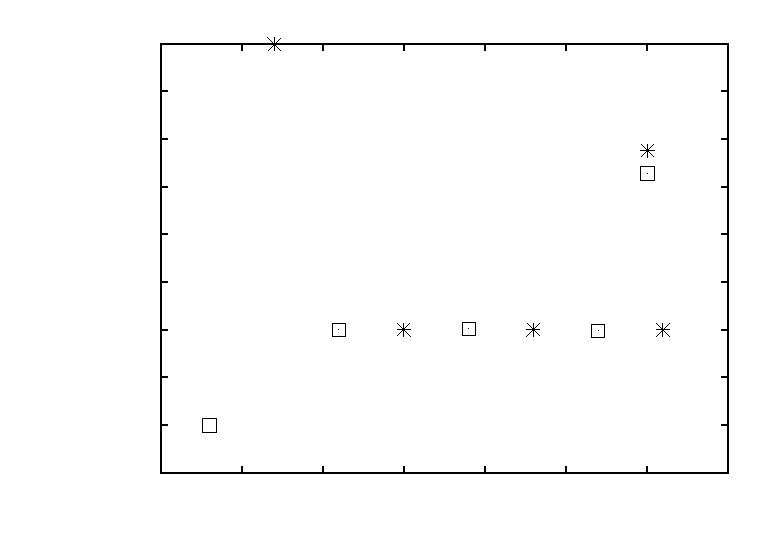
\includegraphics{fig/sleep}}%
    \gplfronttext
  \end{picture}%
\endgroup

    \caption{Tempo de dorm�ncia com chamadas \cod{usleep} de 6 $ms$}
    \label{fig:sleep}
  \end{center}
\end{figure}

Observa-se que, nas duas execu��es, depois da primeira chamada, os processos sempre
dormem $8 ms$, apesar do pedido de $6 ms$ passado para a chamada \cod{usleep}. Isto
� uma conseq��ncia direta do valor do $jiffy$ de $4 ms$, pois $8 ms$ � o menor
m�ltiplo do $jiffy$ maior que $6 ms$.  Observa-se tamb�m que na primeira chamada da
primeira execu��o, o processo chega a dormir $11 ms$ enquanto que na segunda
execu��o, o processo dorme aproximadamente $7 ms$. Este dois cen�rios diferentes
ilustram a depend�ncia do tempo de dorm�ncia no instante relativo no qual a primeira
chamada \cod{usleep} � efetuada em rela��o ao instante no qual o \ing{tick} ocorre,
conforme explicado no in�cio desta se��o.

� importante observar que a variabilidade discutida nesta se��o caracteriza o
comportamento do escalonador do Linux. No contexto deste trabalho, esta
variabilidade n�o tem relev�ncia, pois as plataformas de tempo real estudas
utilizam um escalonador pr�prio, baseados em temporizadores de alta
precis�o. Portanto, a variabilidade de escalonamento n�o foi contemplada nos
experimentos, pois n�o serve para efeito de compara��o. No entanto, escolheu-se
apresentar esta conseq��ncia da exist�ncia do \ing{tick} devido � sua import�ncia na
implementa��o dos SO modernos.


\subsection{Lat�ncia de interrup��o}
\label{sec:latIRQ}

Como foi visto na se��o \ref{sec:interrupt}, as interrup��es de hardware s�o
ass�ncronas e podem acontecer em qualquer momento do ciclo de execu��o do
processador. Al�m disso, a execu��o da parte cr�tica de um tratador de interrup��o
requer eventualmente a desabilita��o das interrup��es para impedir o acesso concorrente a
dados protegidos por \ing{spin-locks} dentro de tratadores de interrup��o.

Portanto, quando uma interrup��o acontece, v�rios cen�rios de lat�ncia para a sua
detec��o e seu tratamento pelo processador s�o poss�veis. Se as interrup��es forem
habilitadas, ela � detectada no final do ciclo das instru��es em execu��o. Sen�o, a
interrup��o pode acontecer enquanto as interrup��es est�o desabilitadas pela execu��o
da parte cr�tica de um tratador de interrup��o. Ap�s o fim da execu��o deste
tratador, as interrup��es voltam a ser habilitadas novamente.

Em seguida � detec��o da interrup��o, o processador come�a por gravar o contador de
programa e alguns registradores da mem�ria para poder retomar a execu��o do processo
interrompido, depois do tratamento da interrup��o. Observe que um tratador de
interrup��o executa no contexto do �ltimo processo executado. Conseq�entemente, a
troca de contexto necess�ria para executar o tratador no processador � bastante
r�pida.  Depois de executar mais algumas opera��es, tal como ler o vetor de
interrup��o no controlador de interrup��o e carregar as informa��es necess�rias no
seus registradores, o processador finalmente come�a a executar o tratador da interrup��o
que aconteceu. O tempo decorrido entre o instante no qual a interrup��o aconteceu e
o in�cio da execu��o do tratador associado � chamado de \textbf{lat�ncia de
  interrup��o} (\ing{interrupt latency}).

A lat�ncia de interrup��o caracteriza a capacidade do sistema para reagir a eventos 
externos. Portanto, esta grandeza foi contemplada como m�trica para 
efeito de compara��o das plataformas estudas (ver se��o \ref{sec:experimentos}).


\subsection{Lat�ncia de ativa��o}
\label{sec:latAtiv}

Quando uma interrup��o ocorre, quer seja porque um temporizador expirou ou porque um
evento de hardware ocorreu, o tratador da interrup��o executa imediatamente a parte
cr�tica.  Lembrar que a palavra cr�tica faz aqui refer�ncia �s primitivas de
sincroniza��o e as estruturas de dados utilizadas, no contexto de um sistema
preempt�vel e com acesso concorrente aos dados (ver se��o \ref{sec:interrupt}).  A
parte n�o-cr�tica do tratador � executada num \ing{softirq} logo ap�s o retorno da
parte cr�tica do tratador.  No entanto, entre o instante no qual a interrup��o
ocorre e o instante no qual o \ing{softirq} come�a a executar, outras interrup��es
podem acontecer, provocando um poss�vel atraso na execu��o da parte n�o-cr�tica.

Nas plataformas de tempo real, eventos de temporizadores ou de \ing{hardware} s�o
utilizados para disparar tarefas, num modelo similar aos \ing{softirqs}. Tal tarefa,
muitas vezes peri�dica, tem um contexto pr�prio e fica suspensa, na espera de um
evento.  Quando o evento ocorre, a interrup��o associada aciona o seu tratador, que,
por sua vez, acorda a tarefa. O intervalo de tempo entre os instantes no qual o
evento ocorre e o in�cio da execu��o da tarefa associada � chamada de
\textbf{lat�ncia de ativa��o}.  Assim como no caso dos \ing{softirqs}, a lat�ncia de
ativa��o pode ser aumentada pela ocorr�ncia de interrup��es. Al�m disso, a execu��o
de outros \ing{softirqs} pode ser escalonada com alguma pol�tica (ex: FIFO,
prioridade fixa), o que pode tamb�m gerar interfer�ncias na lat�ncia de ativa��o.

Um outro aspecto importante diz respeito � implementa��o dos temporizadores
utilizados para agendar as tarefas de tempo real. Mais especificamente, a obten��o
de uma precis�o de micro-segundos nos eventos disparados por temporizadores requer a
utiliza��o de rel�gios de alta precis�o, distintos daqueles usados pelo \kernell
padr�o. Desta forma, a lat�ncia de ativa��o passa a ser independente do escalonador
de processos do Linux e do valor do \cod{jiffy}.

Assim como a lat�ncia de interrup��o, a lat�ncia de ativa��o caracteriza a
capacidade de um sistema em reagir aos eventos externos.  Portanto, esta grandeza foi
tamb�m contemplada com m�trica para efeito de compara��o das plataformas estudas
(ver se��o \ref{sec:experimentos}).


\subsection{Lat�ncia causada pela invers�o de prioridade}
\label{sec:invPrior}

Para organizar o compartilhamento dos recursos, os processos utilizam as primitivas
de \ing{locks} que foram descritas na se��o \ref{sec:locks}.  Quando um processo
quer obter o acesso a um recurso, ele adquire o \ing{lock} associado. Uma vez em
posse do \ing{lock}, um processo utiliza o recurso e, em algum momento futuro,
devolve o \ing{lock} quando ela n�o precisa mais do recurso.

Este mecanismo de reserva pode causar lat�ncia de ativa��o em contradi��o com as
pol�ticas de prioridades definida no sistema. Considere-se, primeiramente, um
cen�rio envolvendo dois processos $P_A$ e $P_B$, o primeiro de alta prioridade e o
segundo de baixa prioridade. Suponha que $P_B$ adquire um recurso compartilhado $R$,
e que, enquanto $P_B$ est� utilizando $R$, uma interrup��o de \ing{hardware} acorda
$P_A$. Ent�o, $P_A$ causa a preemp��o de $P_B$ e adquire o processador.
Possivelmente, $P_A$ tenta adquirir o \ing{lock} do recurso $R$. Por�m, $P_B$ n�o
liberou o \ing{lock} ainda e, conseq�entemente, $P_A$ tem que esperar que $P_B$
ganhe o processador novamente e complete a sua execu��o, pelo menos at� devolver o
\ing{lock}.  S� ent�o $P_A$ pode adquirir o processador e conseguir o recurso
$R$. Percebe-se que, neste cen�rio, o processo de mais alta prioridade acaba
esperando pelo processo de mais baixa prioridade.

Esta situa��o simples pode se tornar ainda pior no seguinte caso.  Suponha agora que
um (ou mais) processo $P_{M}$ de prioridade m�dia, mais alta que a prioridade de
$P_B$ e mais baixa que a prioridade de $P_A$ comece a executar enquanto $P_B$ est�
em posse do recurso $R$. $P_A$ n�o pode executar enquanto $P_B$ n�o libera o recurso
$R$ e $P_B$ n�o pode executar enquanto $P_{M}$ n�o libera o processador. Portanto, o
processo de mais alta prioridade pode ficar esperando um tempo indefinido, enquanto
tiver processos de prioridade intermedi�ria ocupando o processador.

Duas solu��es para este problema, chamado de invers�o de prioridade, foram propostas
por Sha et al em 1990 num trabalho pioneiro \cite{Sha90}. A primeira utiliza o
conceito de heran�a de prioridade.  Resumidamente, enquanto um processo de baixa
prioridade utiliza um recurso, ele herda a prioridade do processo de maior
prioridade que est� esperando por aquele recurso.  Desta forma, e na aus�ncia de
bloqueios encadeados, o tempo m�ximo que um processo de alta prioridade ter� de
esperar � o tempo m�ximo que um processo de mais baixa prioridade pode bloquear o
recurso.  A segunda solu��o consiste em determinar em tempo de projeto, a mais alta
prioridade dos processos que compartilham um certo recurso. Esta prioridade teto
ser� ent�o atribu�da a qualquer um destes processos durante sua utiliza��o deste
recurso.  Apesar de n�o impedir a invers�o de prioridade, estas solu��es permitem
limitar o tempo m�ximo de espera de um processo de mais alta prioridade no sistema,
aumentando, portanto, o grau de previsibilidade do sistema.  Outras solu��es s�o
baseadas em protocolos sem \ing{locks} ou na replica��o dos recursos
\cite{Tanenbaum01}.

A ocorr�ncia de invers�o de prioridade depende altamente das aplica��es e do uso que
elas fazem dos recursos compartilhados. Al�m disso, as lat�ncias por invers�o de prioridade
sofridas pelas aplica��es resultam tamb�m das lat�ncias de interrup��o e de
ativa��o. Ambos os fatos dificultam a elabora��o de experimentos de medi��o. Portanto,
esta grandeza n�o foi utilizada como m�trica no contexto deste cap�tulo.


\section{Solu��es de SOTR baseadas em Linux} %5
\label{sec:sotrLinux}

Nesta se��o, apresentaremos os princ�pios de tr�s abordagens diferentes para tornar
o Sistema Operacional Linux de Tempo Real. A primeira, descrita na se��o
\ref{sec:preemptRT}, consiste em tornar o \kernell Linux inteiramente
preempt�vel. Desta forma, � poss�vel limitar as lat�ncias m�ximas de interrup��o e
de ativa��o.  Uma outra abordagem, descrita na se��o \ref{sec:sandbox}, consiste em
organizar a ativa��o das tarefas de tempo real a partir dos tratadores de
interrup��o, criando uma interface de programa��o acess�vel em modo usu�rio.
Finalmente, uma terceira abordagem, baseada em \nanokernel, ser� descrita na se��o
\ref{sec:nanokernel}. Esta proposta utiliza uma camada intermedi�ria entre o
\kernell e o hardware, o \nanokernel, que oferece servi�os de tempo real para as
aplica��es.  Apesar de existir em outras propostas de SOTR baseadas no Linux (ex:
\cite{Barabanov97, Srinivasan98, Calandrino06}), estas tr�s abordagens s�o
bastante representativas para permitir a exposi��o dos princ�pios
fundamentais destinados ao aumento da previsibilidade de um SOPG tal como Linux.


\subsection{O \ing{patch} \preempt}
\label{sec:preemptRT}

H� alguns anos, Ingo Molnar, juntamente com outros desenvolvedores do \kernell Linux
\cite{McKenney05, Rostedt07}, t�m trabalhando ativamente para que o pr�prio
\kernell possa oferecer servi�os de tempo real confi�veis. Este trabalho resultou na
publica��o do \ing{patch} do \kernell chamado ``\preempt'' em abril de
2006 e cujo c�digo est� dispon�vel na internet \cite{PreemptRT}.

Para resolver o problema da precis�o temporal do escalonador baseado em \ing{ticks}
descrito na se��o \ref{sec:latEscal}, o \ing{patch} \preemptt utiliza uma nova
implementa��o dos temporizadores de alta resolu��o desenvolvida por Thomas Gleixner
e documentada no pr�prio c�digo do \kernell Linux \cite{Kernel}. Baseados no
registrador \ing{Time Stamp Counter} (TSC) da arquitetura Intel ou em rel�gios de
alta resolu��o, esta implementa��o oferece uma API que permite obter valores
temporais com uma resolu��o de micro-segundos. Desde a vers�o do \kernell 2.6.21,
esta API faz parte da linha principal do \kernel.  De acordo com resultados
apresentados \cite{Rostedt07}, os tempos de lat�ncia de ativa��o obtidos usando esta
API s�o da ordem de algumas dezenas de micro-segundos e n�o dependem mais da
freq��ncia do \ing{tick}. Com \preempt, o \ing{tick} continua sendo estritamente
peri�dico.  No entanto, com a proposta do KURT-Linux \cite{Srinivasan98}, que
disponibiliza o \ing{patch} $UTIME$, � poss�vel utilizar um \ing{tick} aperi�dico e
program�vel com uma resolu��o de alguns micro-segundos.

O segundo problema diz respeito aos tempos de lat�ncia de interrup��o e de
preemp��o.  Al�m de utilizar temporizadores de alta precis�o, o \ing{patch}
\preemptt comporta v�rias modifica��es para tornar o \kernell totalmente
preempt�vel. Este objetivo � essencial para garantir que, quando um processo de mais
alta prioridade acorda, ele consiga adquirir o processador com uma lat�ncia m�nima,
sem ter que esperar o fim da execu��o de um processo de menor prioridade, mesmo que
este esteja executando em modo \kernel.  Como foi visto nas se��es
\ref{sec:locks} e \ref{sec:latIRQ}, a utiliza��o das primitivas de sincroniza��o que
permitem garantir a exclus�o m�tua de regi�es cr�ticas introduz poss�veis fontes de
lat�ncia e indeterminismo. Para eliminar estas fontes de imprevisibilidade,
\preemptt modifica estas primitivas de maneira a permitir a implementa��o de um
protocolo complexo, baseado em heran�a de prioridade. Por exemplo, um \ing{spin-lock}
(ou um \ing{mutex}) agora possui um dono, uma fila de processos em espera e pode sofrer
preemp��o, ou seja, um processo possuindo um \ing{spin-lock} pode ser suspenso.  Os
atributos dono e fila s�o necess�rios para a implementa��o do protocolo baseado em
heran�a de prioridade \cite{Sha90}, como foi visto na se��o \ref{sec:compTemp}.

Uma outra modifica��o importante diz respeito ao tratamento das interrup��es. No
\kernell padr�o, quando uma interrup��o acontece, a parte cr�tica do tratador da
interrup��o � executada logo que a interrup��o � detectada pelo processador, podendo,
 conseq�entemente, atrasar a execu��o de um outro tratador ou processo de maior
prioridade. Para diminuir esta causa de lat�ncia, o \ing{patch} \preemptt utiliza
\ing{threads} de interrup��es. Quando uma linha de interrup��o � inicializada, um
\ing{thread} � criado para gerar as interrup��es associadas a esta linha.  Na
ocorr�ncia de uma interrup��o, o tratador associado simplesmente mascara a
interrup��o, acorda o \ing{thread} da interrup��o e volta para o c�digo
interrompido. Desta forma, a parte cr�tica do tratador de interrup��o � reduzida ao
seu m�nimo e a lat�ncia causada pela sua execu��o, al�m de ser breve, �
determin�stica. O \ing{thread} acordado ser� eventualmente escalonado, de acordo com
a sua prioridade e os demais processos em execu��o no processador.
 
De acordo com os resultados obtidos \cite{Rostedt07, Siro07}, o \ing{patch}
\preemptt permite reduzir as lat�ncias do \kernell padr�o para valores da ordem de
algumas dezenas de micro-segundos.  Portanto, usando c�digos confi�veis, respeitando
as regras de programa��o do \ing{patch} e alocando os recursos de acordo com os
requisitos temporais, a solu��o \preemptt tem a vantagem de oferecer o ambiente de
programa��o do sistema Linux, dando acesso �s bibliotecas C e ao conjunto de
software dispon�vel para este sistema.


\subsection{Uma caixa de areia em espa�o usu�rio}
\label{sec:sandbox}

A proposta de caixa de areia \cite{Qi04, Fry07} tem o objetivo de permitir a
extens�o do \kernell Linux padr�o para oferecer uma interface de programa��o para
tarefas de tempo real executadas em modo usu�rio. A id�ia fundamental aplicada aqui
� criar uma extens�o do espa�o de mem�ria de todos os processos executados no
sistema. Esta implementa��o utiliza o gerenciamento por p�ginas da mem�ria virtual e
n�o requer nenhum dispositivo de hardware espec�fico. Basicamente, uma caixa de
areia corresponde a uma ou duas p�ginas da mem�ria virtual que s�o adicionadas a
todas as �reas de mem�ria dos processos do sistema.  Desta forma, qualquer c�digo da
caixa de areia pode ser executado em modo usu�rio no contexto de qualquer processo.

Para oferecer as extens�es da caixa de areia, o \kernell � modificado atrav�s de
m�dulos carregados, cujas funcionalidades s�o utilizadas via \ing{ioctls}, de uma
forma semelhante aos controladores de dispositivos. Atrav�s da interface de
programa��o, um processo $P$ pode registrar servi�os na caixa de areia. Para utilizar
estes servi�os, por exemplo, durante a execu��o de um tratador de interrup��o, o \kernell usa
uma fun��o de \ing{upcall} que acorda um \ing{thread} previamente criado pelo
processo $P$. Este \ing{thread} executa em modo usu�rio, no contexto do �ltimo
processo que estava executando no processador. Como este processo, possivelmente
diferente de $P$, tem a caixa de areia na sua �rea de mem�ria virtual, o
\ing{thread} acordado tem acesso a todas as funcionalidades registradas nesta �rea
de mem�ria compartilhada.

O tamanho da caixa de areia � arbitr�rio, mas deve ser suficiente para comportar uma
pilha de execu��o dos \ing{thread} e para conter uma vers�o pequena da biblioteca C
padr�o. Para isto, duas p�ginas de $4 Mb$ s�o utilizadas.  Uma p�gina, chamada
``p�blica'', d� direito de leitura e execu��o, tanto em modo usu�rio quanto em modo
\kernel. Esta p�gina cont�m as fun��es da interface de programa��o e as fun��es
registradas pelos processos quando eles s�o criados. A outra p�gina, dita
``protegida'', d� direito de leitura e escrita em modo \kernel, mas s� pode ser
escrita por um \ing{thread} executando em modo usu�rio durante um \ing {upcall}.
Isto garante que os dados de um processo, contidos na caixa de areia, n�o podem ser
alterados por outros processos.

Nesta implementa��o, os servi�os da caixa de areia s�o obtidos a partir da parte n�o
cr�tica do tratador de interrup��o (\ing{softirq}). Apesar de esta parte dos
tratadores ser executada com certa imprevisibilidade comparativamente com a parte
cr�tica, esta escolha � justificada pelos autores pelo fato de permitir aos c�digos
da caixa de areia fazerem chamadas de sistemas bloqueantes. Resultados apresentados
mostram que os tempos de lat�ncia de interrup��o s�o da ordem de dezenas de
micro-segundos, inclusive no caso de interrup��es geradas pela placa de rede na
recep��o de mensagens Ethernet. No entanto, no caso de eventos de redes, os autores
produzem desvios padr�es da mesma ordem de grandeza que as lat�ncias medidas.
Apesar deste fato, o uso da caixa de areia � advogado pelos autores \cite{Fry07}
para sistemas de tempo real n�o-cr�ticos. No contexto deste trabalho, esta solu��o n�o
foi contemplada, pois \doriss tem requisitos de tempo real cr�ticos.


\subsection{\emph{Nanokernel}}
\label{sec:nanokernel}

As solu��es de implementa��o para SOTRs baseadas em \nanokernel, sendo as mais
divulgadas RT-Linux \cite{Barabanov97, rtLinux}, \ing{Real Time Application
  Interface} (RTAI) \cite{Dozio03, RTAI} e Xenomai \cite{Gerum05, Xenomai} s�o as
�nicas, at� o momento, que alcan�am lat�ncias da ordem do micro-segundos e d�o
suporte a sistemas cr�ticos. Estas solu��es utilizam uma camada de indire��o das
interrup��es, chamada camada de abstra��o do hardware (HAL), localizada entre o
\ing{kernel} e os dispositivos de hardware e disponibilizam uma interface de
programa��o para servi�os de tempo real. Observa-se que os c�digos fontes do Xenomai
e RTAI s�o dispon�veis sob licen�a GNU/GPL. No caso do RT-Linux, uma vers�o
profissional � desenvolvida sob licen�a comercial. Uma outra vers�o livre �
disponibilizada, sob licen�as espec�ficas, com uma interface de utiliza��o restrita
e sem suporte para as vers�es do \kernell posteriores a 2.6.9.

Do ponto de vista da implementa��o,  os \nanokernell de Xenomai, RTAI e RT-Linux
utilizam o mecanismo de virtualiza��o das interrup��es, tamb�m chamada de indire��o
de interrup��o, introduzido na t�cnica de ``prote��o otimista das interrup��es''
\cite{Stodolsky93}. No contexto da intera��o do \nanokernell com Linux, esta t�cnica
pode ser resumida da seguinte maneira. Quando uma interrup��o acontece, o
\nanokernell identifica se esta � relativa a uma tarefa de tempo real ou se a
interrup��o � destinada a um processo do \kernell Linux. No primeiro caso, o
tratador da interrup��o � executado imediatamente. Caso contr�rio, a interrup��o �
enfileirada e, em algum momento futuro, entregue para o \kernell Linux quando
nenhuma tarefa de tempo real estiver precisando executar. Quando o \kernell Linux
precisa desabilitar as interrup��es, o \nanokernell deixa o \kernell Linux acreditar
que as interrup��es est�o desabilitadas. No entanto, o \nanokernell continua a
interceptar qualquer interrup��o de \ing{hardware}.  Nesta ocorr�ncia, a interrup��o
� tratada imediatamente se for destinada a uma tarefa de tempo real. Caso contr�rio,
a interrup��o � enfileirada, at� que o \kernell Linux habilite suas interrup��es
novamente.


\subsubsection{RT-Linux}

No caso da vers�o livre do RT-Linux, tanto a camada HAL quanto API de programa��o
s�o fornecidas em um �nico \ing{patch} que modifica o c�digo fonte do \kernell
Linux. Este \ing{patch} permite ent�o co-exist�ncia do \nanokernell RT-Linux que
oferece garantias temporais cr�ticas para as tarefas de tempo real e do \kernell
Linux padr�o. O modelo de programa��o das tarefas de tempo real � baseado na
inser��o de m�dulos no \kernell em tempo de execu��o.  Portanto, estas tarefas devem
necessariamente executar em modo protegido, o que restringe a interface de
programa��o fornecida pelo RT-Linux.

Para realizar a virtualiza��o das interrup��es, as fun��es que manipulam as
interrup��es \cod{local\_irq\_enable}, antigamente \cod{sti} (\ing{set
  interruption}) e \cod{local\_irq\_disable}, antigamente \cod{cli} (\ing{clear
  interruption}), s�o modificadas. Para dar o controle � camada HAL, as novas
fun��es n�o alteram mais a m�scara real de interrup��o, mas utilizam uma m�scara
virtual.  Enquanto esta m�scara virtual indicar que as interrup��es s�o
desabilitadas, depois de uma chamada \cod{local\_irq\_disable} pelo \kernell Linux,
o \nanokernell intercepta as interrup��es que n�o s�o de tempo real e trata as
interrup��es de tempo real imediatamente. Quando o \kernell chama a fun��o
\cod{local\_irq\_disable}, a m�scara virtual de interrup��o � modificada e o
\nanokernell entrega as interrup��es pendentes para Linux.

Resumindo, no RT-Linux, o \ing{kernel} Linux � uma tarefa escalonada pelo
\nanokernell RT-Linux como se fosse a tarefa de mais baixa prioridade no sistema.

\subsubsection{Adeos, RTAI e Xenomai}
\label{sec:adeos}

No caso dos projetos RTAI \cite{Dozio03} e Xenomai \cite{Gerum05}, a camada HAL �
fornecida pelo \ing{Adaptative Domain Environment for Operating Systems} (Adeos),
desenvolvida por Karim Yaghmour \cite{Yaghmour01}.  Adeos, fornecida por um
\ing{patch} separado, tem os seguintes objetivos:

\begin{itemize}
\item permitir o compartilhamento dos recursos de hardware entre diferentes sistemas
  operacionais e/ou aplica��es espec�ficas;
\item contornar a padroniza��o dos SO, isto �, flexibilizar o uso do hardware para
  devolver o controle aos desenvolvedores e administradores de sistema;
\item oferecer uma interface de programa��o simples e independente da arquitetura.
\end{itemize}

Para n�o ter que iniciar a constru��o de um sistema operacional de tempo real
completo, o \nanokernell Adeos utiliza Linux como hospedeiro para iniciar o
hardware. Logo no in�cio, a camada Adeos � inserida abaixo do \kernell Linux para
tomar o controle do hardware.  Ap�s isto, os servi�os de Adeos podem ser utilizados
por outros sistemas operacionais e/ou aplica��es executando conjuntamente ao
\kernell Linux.

A arquitetura Adeos utiliza dois conceitos principais, dom�nio e canal hier�rquico
de interrup��o. Um dom�nio caracteriza um ambiente de execu��o isolado, no qual se
pode executar programas ou at� mesmo sistemas operacionais completos.  Dom�nios
diferentes s�o associados ao SO Linux e �s aplica��es mais espec�ficas como RTAI ou
Xenomai.  Um dom�nio enxerga Adeos mas n�o enxerga os outros dom�nios hospedados no
sistema.

O canal hier�rquico de interrup��o, chamado \ing{ipipe}, serve para priorizar a
entrega de interrup��es entre os dom�nios.  Quando um dom�nio se registra no Adeos,
ele � colocado numa posi��o no \ing{ipipe} de acordo com os seus requisitos
temporais.  Adeos utiliza ent�o o mecanismo de virtualiza��o das interrup��es para
organizar a entrega hier�rquica das interrup��es, come�ando pelo dom�nio mais
priorit�rio e seguindo com os menos priorit�rios.  Fun��es apropriadas
(\ing{stall/unstall}) permitem bloquear ou desbloquear a transmiss�o das
interrup��es atrav�s de cada dom�nio.

Para prover servi�os de tempo real, as interfaces RTAI ou Xenomai utilizam o dom�nio
mais priorit�rio do \ing{ipipe}, chamado ``dom�nio prim�rio''. Este dom�nio
corresponde, portanto, ao n�cleo de tempo real no qual as tarefas s�o executadas em
modo protegido. Como as interrup��es s�o entregues come�ando pelo dom�nio prim�rio,
o n�cleo de tempo real pode escolher atrasar, ou n�o, a entrega das interrup��es
para os demais dom�nios registrados no \ing{ipipe}, garantindo, desta forma, a execu��o
das suas pr�prias tarefas. M�dulos podem ser utilizados para carregar as tarefas, de
forma semelhante ao RT-Linux. 

Nas plataformas Xenomai e RTAI, o ``dom�nio secund�rio'' corresponde ao \kernell
Linux.  Neste dom�nio, o conjunto de bibliotecas e software usual do Linux est�
dispon�vel.  Em contrapartida, as garantias temporais s�o mais fracas, dado que o
c�digo pode utilizar as chamadas de sistemas bloqueantes do Linux.

Para oferecer o servi�o de tempo real em modo usu�rio chamado LXRT, RTAI utiliza o
mecanismo de associa��o (\ing{shadowing}) de um \ing{thread} do n�cleo de tempo real
com um processo usu�rio executando no dom�nio Linux. De acordo com sua prioridade,
este \ing{thread}, tamb�m chamado de ``sombra'' do processo, executa o escalonamento
r�pido do seu processo associado.

O projeto Xenomai se distingue do RTAI/LXRT. Al�m de n�o utilizar o mecanismo de
associa��o (\ing{shadowing}), Xenomai tem por objetivo privilegiar o modelo de
programa��o em modo usu�rio. O modelo de tarefas executando no modo protegido s�
est� sendo mantido para dar suporte �s aplica��es legadas. A implementa��o dos
servi�os de tempo real em modo usu�rio se baseia nas seguintes regras:

\begin{itemize}
\item A pol�tica de prioridade utilizada para as tarefas de tempo real, e para o
  escalonador associado, � comum aos dois dom�nios.
\item As interrup��es de hardware n�o podem impedir a execu��o de uma tarefa
  priorit�ria enquanto ela estiver no dom�nio secund�rio.
\end{itemize}

A primeira destas garantias utiliza um mecanismo de heran�a de prioridade entre o
dom�nio prim�rio e o dom�nio secund�rio.  Quando uma tarefa do dom�nio prim�rio
migra para o secund�rio, por exemplo, porque ela efetua uma chamada de sistema do
Linux, esta tarefa continua com a mesma prioridade, maior que a de qualquer processo
do Linux.  Este mecanismo garante notadamente que a preemp��o de uma tarefa de tempo
real executando no dom�nio secund�rio n�o possa ser causada por uma tarefa de menor
prioridade executando no dom�nio prim�rio. A segunda garantia � obtida por meio de
um dom�nio intermedi�rio, chamado de ``escudo de interrup��o'', registrado no
\ing{ipipe}, entre o primeiro dom�nio (o \nanokernell) e o segundo dom�nio (o
\kernell Linux).  Enquanto uma tarefa de tempo real est� executando no segundo
dom�nio, o ``escudo de interrup��o'' � utilizado para bloquear as interrup��es de
hardware destinadas ao Linux. No entanto, aquelas interrup��es destinadas � tarefa
em execu��o s�o entregues imediatamente.

Para completar esta arquitetura, as chamadas de sistema executadas por uma tarefa
enquanto est� no dom�nio prim�rio e secund�rio s�o interceptadas por Adeos que
determina a fun��o a ser executada, seja ela do Linux padr�o ou da API do 
Xenomai. Isto permite que uma tarefa executando no dom�nio secund�rio possa
obter os servi�os providos por Xenomai.

Observa-se que quando uma tarefa est� no dom�nio secund�rio, ela pode sofrer uma
lat�ncia de escalonamento devido � execu��o de alguma sess�o n�o preemptiva do
Linux. Portanto, Xenomai se beneficia do esfor�o de desenvolvimento do
\ing{patch} \preempt, que tem por objetivo tornar o \kernell inteiramente
preempt�vel.  Apesar de ainda constituir um \ing{patch} separado, v�rias propostas
do grupo de desenvolvedores deste \ing{patch} j� foram integrados na linha principal
do \kernell 2.6, melhorando significativamente suas capacidades de preemp��o.



\section{Metodologia experimental}
\label{sec:experimentos}


Em geral, realizar medi��es precisas de tempo no n�vel dos tratadores
de interrup��o pode n�o ser t�o simples.  De fato, o instante exato no
qual uma interrup��o acontece � de dif�cil medi��o, pois tal evento �
ass�ncrono e pode ser causado por qualquer dispositivo de \ing{hardware}. Para
obter medidas das lat�ncias de interrup��o e ativa��o confi�veis com
alto grau de precis�o, aparelhos externos, tais como oscilosc�pios ou
outros computadores, s�o necess�rios. No entanto, como o objetivo do
presente trabalho n�o foi medir estas lat�ncias de forma precisa, mas
caracterizar e comparar o grau de determinismo das plataformas
operacionais estudadas, adotou-se uma metodologia experimental simples
e efetiva, que pode ser reproduzida facilmente em outros contextos.

\subsection{Configura��o do experimento}

O dispositivo experimental utilizou tr�s esta��es: (1) a esta��o de
medi��o $E_M$, na qual os dados foram coletados e onde temos uma
tarefa de tempo real $\tau$ � espera de eventos externos; (2) a
esta��o de disparo $E_D$, que foi utilizada para enviar pacotes
Ethernet com uma freq��ncia fixa � esta��o $E_M$; e (3) a esta��o de
carga $E_C$, utilizada para criar uma carga de interrup��o na esta��o
$E_M$. As esta��es de disparo e carga foram conectadas � esta��o de
medi��o por duas redes Ethernet distintas, conforme ilustrado no
diagrama da figura \ref{fig:config}.


\begin{figure}[hbt]
  \centering {\scalebox{1}{\input{fig/config.pstex_t}}}
  \caption{Configura��o do experimento.} \label{fig:config}
\end{figure}

As chegadas em $E_M$ dos pacotes enviados por $E_D$ servem para disparar uma cascata
de eventos na esta��o $E_M$, permitindo a simula��o de eventos externos via a porta
paralela (PP). Mais explicitamente, cada chegada de um pacote Ethernet na placa foi
utilizada para disparar uma interrup��o na PP, escrevendo no pino de interrup��o
desta porta. Esta escrita foi realizada pelo pr�prio tratador $T_{eth}$ de
interrup��o da placa de rede de $E_M$.  O instante $t_1$ de escrita no pino de
interrup��o da PP pelo tratador $T_{eth}$ constitui ent�o o in�cio da seq��ncia de
eventos utilizados para medir as lat�ncias de interrup��o ($Lat_{irq}$) e de ativa��o
($Lat_{ativ}$).

\begin{figure}[hbt]
  \centering {\scalebox{1}{\input{fig/dispExp.pstex_t}}}
  \caption{C�lculo das lat�ncias de interrup��o e ativa��o na esta��o
    $E_M$.} \label{fig:dispExp}
\end{figure}


As medidas de lat�ncia foram realizadas pela consulta do contador do
processador, chamado \ing{Time Stamp Counter} (TSC), permitindo uma
precis�o da ordem de micro-segundos. Concretamente, um m�dulo
espec�fico ($M$) foi desenvolvido na esta��o $E_M$ para exportar as
funcionalidades seguintes:

\begin{itemize}
\item Ler os 64 bits do TSC e armazenar o valor lido na mem�ria.
\item Escrever na porta de entrada e sa�da 0x378 da porta paralela para gerar
  interrup��es de hardware.
\item Criar uma tarefa $\tau$ que, num sistema real, executaria algum c�digo �til
  precisando de garantias de tempo real cr�tico. Neste experimento, $\tau$
  simplesmente grava o valor do TSC.
\item Requisitar a captura das interrup��es na linha 7 associada � porta paralela e
  registrar o tratador de interrup��o $T_{PP}$ associado.
\item Definir o tratador $T_{PP}$ que executa as duas opera��es seguintes: (1)
  gravar o TSC; (2) acordar tarefa $\tau$.
\item Criar um canal de comunica��o FIFO ass�ncrono para a transfer�ncia dos dados
  temporais coletados em modo protegido para o espa�o usu�rio.
\end{itemize}

Parte deste conjunto de fun��es foi disponibilizado sob forma de \cod{ioctl} para os
processos executando em modo usu�rio atrav�s de um arquivo especial \cod{/dev/M} do
sistema de arquivos. A outra parte foi diretamente exportada, sob a forma de servi�os do
\kernell podendo ser utilizados somente por \ing{threads} do \kernel. 

As medidas seguiram o seguinte roteiro, ilustrado pela figura \ref{fig:dispExp}:

\begin{itemize}
\item A esta��o $E_D$ envia pacotes Ethernet para a esta��o $E_M$, provocando
  interrup��es ass�ncronas em rela��o �s aplica��es executando em $E_M$.
\item A interrup��o associada � chegada de um pacote provoca a preemp��o da
  aplica��o executando pelo tratador de interrup��o $T_{eth}$.
\item $T_{eth}$ escreve no pino de interrup��o da PP e o instante $t_1$ � armazenado
  na mem�ria.  Este valor $t_1$ corresponde ao valor lido no rel�gio local, no
  instante na escrita da PP, logo ap�s a chegada de uma pacote Ethernet.
\item A interrup��o associada � escrita no pino de interrup��o da PP provoca a
  preemp��o da aplica��o executando pelo tratador de interrup��o $T_{PP}$.
\item $T_{PP}$ grava o instante $t_2$ e acorda a tarefa $\tau$. Este valor $t_2$
  corresponde ao valor do rel�gio local, logo ap�s o in�cio de $T_{PP}$.
\item No momento que a tarefa $\tau$ acorda, ela grava o instante $t_3$ e volta a
  ficar suspensa at� a pr�xima interrup��o na PP. O valor de $t_3$ corresponde ao
  tempo no qual a tarefa $\tau$ come�a a executar, no final da cascata de eventos
  provocada pela chegada de um pacote na placa de rede.
\end{itemize}

Assim como representado na figura \ref{fig:dispExp}, $Lat_{irq}$ corresponde a
diferen�a $t_2 - t_1$ e $Lat_{ativ}$ a diferen�a $t_3 - t_2$.

No decorrer do experimento, a transfer�ncia das medi��es da mem�ria para o sistema
de arquivos � efetuada por um processo usu�rio ($P$) (n�o representado na
figura). Antes de iniciar a fase de medidas, $P$ abre o arquivo especial
\ing{/dev/M} para poder ter acesso �s fun��es \ing{ioctl} disponibilizadas pelo
m�dulo $M$.  $P$ entra ent�o num la�o infinito no qual ele executa a chamada de
sistema \cod{read} para ler os dados do canal FIFO. Enquanto n�o h� dados, $P$ fica
bloqueado.  Em algum momento depois da escrita de dados pela tarefa $\tau$, $P$
acorda, l� o canal e escreve os dados num arquivo do disco r�gido. Tal procedimento
permitiu impedir qualquer interfer�ncia entre a aquisi��o dos dados e seu
armazenamento no sistema de arquivos, pois a execu��o do processo $P$ em modo
usu�rio, n�o interfere na execu��o dos m�dulos do experimento, executados em modo
\kernel.

O mecanismo do disparo das interrup��es na porta paralela pelos eventos de chegada
de pacotes na placa de rede foi utilizado para garantir que estas interrup��es
ocorressem de forma ass�ncrona em rela��o aos processos executando na esta��o de
medi��o. � interessante observar que a interrup��o na porta paralela sempre
acontece logo ap�s a execu��o de $T_{Eth}$. Portanto, a medida da lat�ncia de
interrup��o $Lat_{irq}$ deve ser considerada apenas como indicativa.  No entanto,
ela p�de ser utilizada para o objetivo principal destes experimentos, isto �,
comparar as diferentes plataformas estudadas.

Como foi visto na se��o \ref{sec:latAtiv}, a lat�ncia de ativa��o $Lat_{ativ}$
caracteriza o tempo necess�rio para ativar uma tarefa ap�s a ocorr�ncia do seu
evento de disparo.  O dispositivo apresentado aqui permitiu obter resultados de
acordo como esperado, como ser� visto na se��o \ref{sec:concPlat}. Al�m disso,
o efeito do aumento da atividade na esta��o de medi��o p�de ser investigado, pois o
instante de disparo da interrup��o na porta paralela era totalmente independente da
atividade dos processos na esta��o de medi��o.


\subsection{Cargas de I/O, processamento e interrup��o}
\label{sec:carga}

Num primeiro momento, realizaram-se experimentos com uma carga m�nima no processador
da esta��o de medi��o (modo \ing{single}). Desta forma, observou-se o comportamento
temporal das tr�s plataformas em situa��o favor�vel.  Em seguida, dois tipos de
cargas foram utilizados simultaneamente para sobrecarregar a esta��o de medi��o.
Tais sobrecargas tiveram por objetivo avaliar a capacidade de cada plataforma em
garantir uma lat�ncia determinista no tratamento das interrup��es e na ativa��o de
tarefas de tempo real, apesar da exist�ncia de outras atividades n�o-cr�ticas.  As
cargas de I/O e processamento foram realizadas executando as instru��es seguintes:

\vspace{ 4pt }
% \setstretch{0.94}
\begin{center}
  \framebox[0.8\textwidth]{%
    \begin{minipage}{0.74\linewidth}
      \vspace{ 4pt } \footnotesize{%
        \texttt{while "true"; do\\
          \rule{1cm}{0pt} dd if=/dev/hda2 of=/dev/null bs=1M count=1000\\
          \rule{1cm}{0pt} find / -name ''*.c'' | xargs egrep include\\
          \rule{1cm}{0pt} tar -cjf /tmp/root.tbz2 /usr/src/linux-xenomai\\
          \rule{1cm}{0pt}  cd /usr/src/linux-preempt; make clean; make\\
          done \vspace{ 4pt } %\nolinebreak %\raisebox{10mm}{\rule{0cm}{0.01cm}}
        }}
    \end{minipage}
  }
\end{center}
\vspace{ 4pt }
% \setstretch{1}

Um outro estresse de interrup��o foi criado utilizando uma comunica��o UDP entre a
esta��o $E_M$ configurada como servidor e a esta��o $E_C$ configurada como
cliente. Para isolar esta comunica��o da comunica��o entre $E_M$ e $E_D$,
utilizou-se uma segunda placa de rede em $E_M$, assim com ilustrado pelo diagrama da
figura \ref{fig:dispExp}.  Durante o experimento, o cliente transmitiu pequenos
pacotes de 64 bytes na freq��ncia m�xima permitida pela rede, ou seja, com uma
freq��ncia superior a $200~kHz$ (um pacote a cada $10\mu s$).  Desta forma, mais de
100.000 interrup��es por segundos foram geradas pela segunda placa de rede de $E_M$.
Esta placa de rede foi registrada na linha de interrup��o 18 cuja prioridade � menor
que a prioridade da porta paralela. Portanto, as interrup��es geradas nesta placa de
rede n�o deveriam, a princ�pio, interferir nas lat�ncias de interrup��o mensuradas.

Nos experimentos com cargas, os dois tipos de estresses foram aplicados
simultaneamente e as medi��es s� foram iniciadas alguns segundos depois.


\section{Avalia��o de Linux$^{\mathbf{Prt}}$, Linux$^{\mathbf{Rtai}}$ e
  Linux$^{\mathbf{Xen}}$}
\label{cap:platEstud}

\subsection{Configura��o}

Os experimentos foram realizados em computadores Pentium 4 com processadores de 2.6
Ghz e 512 Mb de mem�ria, com o objetivo de ilustrar o comportamento temporal das
quatro plataformas seguintes:

\begin{description}
\item[$\bullet \;$ Linux$^{\mathbf{Std}}$:] Linux padr�o - \kernell vers�o 2.6.23.9
  (op��o \ing{low-latency});
\item[$\bullet \;$ Linux$^{\mathbf{Prt}}$:] Linux com o \ing{patch}
  \preemptt (rt12) - \kernell vers�o 2.6.23.9.
\item[$\bullet \;$ Linux$^{\mathbf{Rtai}}$:] Linux com o \ing{patch} RTAI - vers�o
  ``magma'' - \kernell vers�o 2.6.19.7;
\item[$\bullet \;$ Linux$^{\mathbf{Xen}}$:] Linux com o \ing{patch} Xenomai - vers�o
  2.4-rc5 - \kernell vers�o 2.6.19.7;
\end{description}

Utilizou-se a configura��o Linux$^{\mathbf{Std}}$ para realizar experimentos de
refer�ncia para efeito de compara��o com as duas plataformas de tempo real
Linux$^{\mathbf{Prt}}$ e Linux$^{\mathbf{Xen}}$.  A vers�o est�vel do \kernell
2.6.23.9, disponibilizada em dezembro de 2007 foi escolhida para o estudo de
Linux$^{\mathbf{Prt}}$, pois este \ing{patch} tem evolu�do rapidamente desde sua
primeira vers�o publicada h� dois anos.  No entanto, utilizou-se a vers�o do
\kernell 2.6.19.7 para o estudo das vers�es ``magma'' de RTAI e 2.4-rc5 de
Xenomai. De fato, considerou-se desnecess�rio atualizar a vers�o do \kernel, pois
RTAI e Xenomai s�o baseadas no Adeos (ver se��o \ref{sec:adeos}) e, portanto, as
garantias temporais oferecidas para as aplica��es executando no primeiro dom�nio
dependem apenas da vers�o de RTAI ou Xenomai e do \ing{patch} Adeos associado, e
n�o, da vers�o do \kernell Linux.

Utilizou-se uma freq��ncia de disparo dos eventos pela esta��o $E_D$ de 20Hz.  Para
cada plataforma, dois experimentos de 10 minutos foram realizados. O primeiro sem
carga nenhuma do sistema e o segundo aplicando os estresses apresentados na se��o
\ref{sec:carga}.  Para a plataforma Linux$^{\mathbf{Xen}}$, o experimento com
estresses foi repetido por uma dura��o de 12 horas.

Para as duas plataformas Linux$^{\mathbf{Rtai}}$ e Linux$^{\mathbf{Xeno}}$, os
diferentes testes de lat�ncias fornecidos foram utilizados, dando resultados menores
que $10\mu s$ no pior caso para a lat�ncia de interrup��o, conforme os padr�es da
arquitetura Intel Pentium 4. Em ambas as plataformas, desabilitaram-se as interrup��es de
gerenciamento do sistema (\ing{SMI}), conforme as recomenda��es dos desenvolvedores
\cite{RTAI, Xenomai}. Isto cancelou uma lat�ncia peri�dica (a cada 32 segundos) de
aproximadamente $2.5ms$ que aparecia nos testes.  No caso das plataformas
Linux$^{\mathbf{Std}}$ e Linux$^{\mathbf{Prt}}$, estas interrup��es foram tamb�m
desabilitadas, por�m, n�o foi constatada nenhuma altera��o das medidas realizadas.


\subsection{Resultados experimentais}
\label{sec:resExp}

Os resultados experimentais s�o apresentados nas figuras
\ref{fig:latIrq} e \ref{fig:latAtiv}, onde o eixo horizontal
representa o instante de observa��o variando de 0 a 60 segundos e o
eixo vertical representa as lat�ncias medidas em micro-segundos. Apesar de
cada experimento ter durado no m�nimo uma hora, escolheu-se apresentar
apenas resultados para um intervalo de $60s$, pois este intervalo �
suficiente para observar o padr�o de comportamento de cada plataforma.
Neste intervalo, o total de eventos por experimentos � 1200, pois a
freq��ncia de chegada de pacotes utilizada foi de $20 Hz$.

Abaixo de cada figura, os seguintes valores s�o indicados: Valor M�dio (VM), desvio
padr�o (DP), valor m�nimo (Min) e valor m�ximo (Max). Estes valores foram obtidos
considerando a dura��o de uma hora de cada experimento. Na medida do poss�vel,
utilizou-se uma mesma escala vertical para todos os gr�ficos.  Conseq�entemente,
alguns valores altos podem ter ficado fora das figuras. Tal ocorr�ncia foi
representada por um tri�ngulo pr�ximo do valor m�ximo do eixo vertical.


\subsubsection{Lat�ncia de interrup��o}
\label{sec:latIrq}


\newcommand{\scaleFact}{0.52}
\newcommand{\spaceFact}{10pt}

\begin{figure}%
  \centering
  \subfloat[\textbf{Linux$^{\mathbf{Std}}$ - Sem carga} \newline
  \vskip 1mm {\footnotesize VM:     8.9, DP:     0.3,  Min:     8.7, Max:    18.4}]{%
    \label{fig:ker23Sem}%
    {\scalebox{\scaleFact}{% GNUPLOT: LaTeX picture with Postscript
\begingroup
  \makeatletter
  \providecommand\color[2][]{%
    \GenericError{(gnuplot) \space\space\space\@spaces}{%
      Package color not loaded in conjunction with
      terminal option `colourtext'%
    }{See the gnuplot documentation for explanation.%
    }{Either use 'blacktext' in gnuplot or load the package
      color.sty in LaTeX.}%
    \renewcommand\color[2][]{}%
  }%
  \providecommand\includegraphics[2][]{%
    \GenericError{(gnuplot) \space\space\space\@spaces}{%
      Package graphicx or graphics not loaded%
    }{See the gnuplot documentation for explanation.%
    }{The gnuplot epslatex terminal needs graphicx.sty or graphics.sty.}%
    \renewcommand\includegraphics[2][]{}%
  }%
  \providecommand\rotatebox[2]{#2}%
  \@ifundefined{ifGPcolor}{%
    \newif\ifGPcolor
    \GPcolorfalse
  }{}%
  \@ifundefined{ifGPblacktext}{%
    \newif\ifGPblacktext
    \GPblacktextfalse
  }{}%
  % define a \g@addto@macro without @ in the name:
  \let\gplgaddtomacro\g@addto@macro
  % define empty templates for all commands taking text:
  \gdef\gplbacktext{}%
  \gdef\gplfronttext{}%
  \makeatother
  \ifGPblacktext
    % no textcolor at all
    \def\colorrgb#1{}%
    \def\colorgray#1{}%
  \else
    % gray or color?
    \ifGPcolor
      \def\colorrgb#1{\color[rgb]{#1}}%
      \def\colorgray#1{\color[gray]{#1}}%
      \expandafter\def\csname LTw\endcsname{\color{white}}%
      \expandafter\def\csname LTb\endcsname{\color{black}}%
      \expandafter\def\csname LTa\endcsname{\color{black}}%
      \expandafter\def\csname LT0\endcsname{\color[rgb]{1,0,0}}%
      \expandafter\def\csname LT1\endcsname{\color[rgb]{0,1,0}}%
      \expandafter\def\csname LT2\endcsname{\color[rgb]{0,0,1}}%
      \expandafter\def\csname LT3\endcsname{\color[rgb]{1,0,1}}%
      \expandafter\def\csname LT4\endcsname{\color[rgb]{0,1,1}}%
      \expandafter\def\csname LT5\endcsname{\color[rgb]{1,1,0}}%
      \expandafter\def\csname LT6\endcsname{\color[rgb]{0,0,0}}%
      \expandafter\def\csname LT7\endcsname{\color[rgb]{1,0.3,0}}%
      \expandafter\def\csname LT8\endcsname{\color[rgb]{0.5,0.5,0.5}}%
    \else
      % gray
      \def\colorrgb#1{\color{black}}%
      \def\colorgray#1{\color[gray]{#1}}%
      \expandafter\def\csname LTw\endcsname{\color{white}}%
      \expandafter\def\csname LTb\endcsname{\color{black}}%
      \expandafter\def\csname LTa\endcsname{\color{black}}%
      \expandafter\def\csname LT0\endcsname{\color{black}}%
      \expandafter\def\csname LT1\endcsname{\color{black}}%
      \expandafter\def\csname LT2\endcsname{\color{black}}%
      \expandafter\def\csname LT3\endcsname{\color{black}}%
      \expandafter\def\csname LT4\endcsname{\color{black}}%
      \expandafter\def\csname LT5\endcsname{\color{black}}%
      \expandafter\def\csname LT6\endcsname{\color{black}}%
      \expandafter\def\csname LT7\endcsname{\color{black}}%
      \expandafter\def\csname LT8\endcsname{\color{black}}%
    \fi
  \fi
  \setlength{\unitlength}{0.0500bp}%
  \begin{picture}(7200.00,5040.00)%
    \gplgaddtomacro\gplbacktext{%
      \csname LTb\endcsname%
      \put(1034,594){\makebox(0,0)[r]{\strut{}$0.0$}}%
      \put(1034,1430){\makebox(0,0)[r]{\strut{}$10.0$}}%
      \put(1034,2267){\makebox(0,0)[r]{\strut{}$20.0$}}%
      \put(1034,3103){\makebox(0,0)[r]{\strut{}$30.0$}}%
      \put(1034,3940){\makebox(0,0)[r]{\strut{}$40.0$}}%
      \put(1034,4776){\makebox(0,0)[r]{\strut{}$50.0$}}%
      \put(1166,374){\makebox(0,0){\strut{}$ 0$}}%
      \put(2109,374){\makebox(0,0){\strut{}$ 10$}}%
      \put(3053,374){\makebox(0,0){\strut{}$ 20$}}%
      \put(3996,374){\makebox(0,0){\strut{}$ 30$}}%
      \put(4939,374){\makebox(0,0){\strut{}$ 40$}}%
      \put(5883,374){\makebox(0,0){\strut{}$ 50$}}%
      \put(6826,374){\makebox(0,0){\strut{}$ 60$}}%
      \put(396,2685){\rotatebox{90}{\makebox(0,0){\strut{}Latency ($\mu s$)}}}%
      \put(3996,110){\makebox(0,0){\strut{}Time ($s$)}}%
    }%
    \gplgaddtomacro\gplfronttext{%
    }%
    \gplbacktext
    \put(0,0){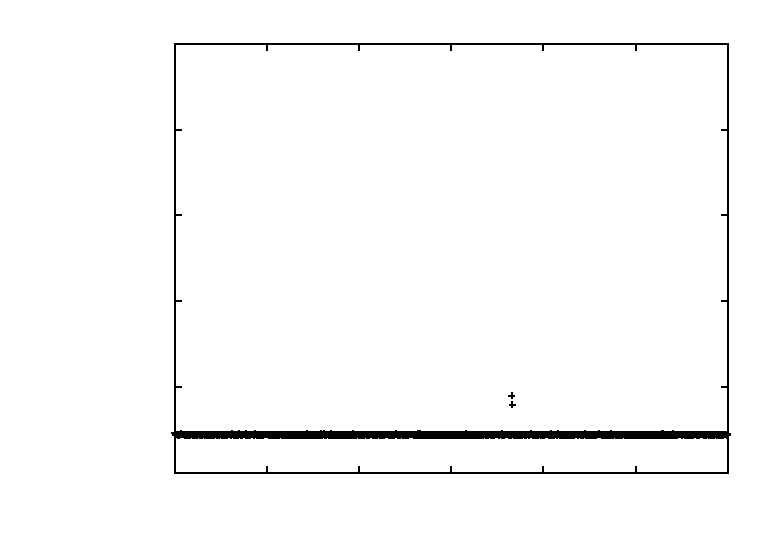
\includegraphics{fig2/ker23Sem}}%
    \gplfronttext
  \end{picture}%
\endgroup
}}} \hspace{4pt}%
  \hspace{\spaceFact}%
  \subfloat[\textbf{Linux$^{\mathbf{Std}}$ - Com carga} \newline
  \vskip 1mm {\footnotesize VM:    10.4, DP:     1.9,  Min:     8.8, Max:    67.7}]{%
    \label{fig:ker23Tot}%
    {\scalebox{\scaleFact}{% GNUPLOT: LaTeX picture with Postscript
\begingroup
  \makeatletter
  \providecommand\color[2][]{%
    \GenericError{(gnuplot) \space\space\space\@spaces}{%
      Package color not loaded in conjunction with
      terminal option `colourtext'%
    }{See the gnuplot documentation for explanation.%
    }{Either use 'blacktext' in gnuplot or load the package
      color.sty in LaTeX.}%
    \renewcommand\color[2][]{}%
  }%
  \providecommand\includegraphics[2][]{%
    \GenericError{(gnuplot) \space\space\space\@spaces}{%
      Package graphicx or graphics not loaded%
    }{See the gnuplot documentation for explanation.%
    }{The gnuplot epslatex terminal needs graphicx.sty or graphics.sty.}%
    \renewcommand\includegraphics[2][]{}%
  }%
  \providecommand\rotatebox[2]{#2}%
  \@ifundefined{ifGPcolor}{%
    \newif\ifGPcolor
    \GPcolorfalse
  }{}%
  \@ifundefined{ifGPblacktext}{%
    \newif\ifGPblacktext
    \GPblacktextfalse
  }{}%
  % define a \g@addto@macro without @ in the name:
  \let\gplgaddtomacro\g@addto@macro
  % define empty templates for all commands taking text:
  \gdef\gplbacktext{}%
  \gdef\gplfronttext{}%
  \makeatother
  \ifGPblacktext
    % no textcolor at all
    \def\colorrgb#1{}%
    \def\colorgray#1{}%
  \else
    % gray or color?
    \ifGPcolor
      \def\colorrgb#1{\color[rgb]{#1}}%
      \def\colorgray#1{\color[gray]{#1}}%
      \expandafter\def\csname LTw\endcsname{\color{white}}%
      \expandafter\def\csname LTb\endcsname{\color{black}}%
      \expandafter\def\csname LTa\endcsname{\color{black}}%
      \expandafter\def\csname LT0\endcsname{\color[rgb]{1,0,0}}%
      \expandafter\def\csname LT1\endcsname{\color[rgb]{0,1,0}}%
      \expandafter\def\csname LT2\endcsname{\color[rgb]{0,0,1}}%
      \expandafter\def\csname LT3\endcsname{\color[rgb]{1,0,1}}%
      \expandafter\def\csname LT4\endcsname{\color[rgb]{0,1,1}}%
      \expandafter\def\csname LT5\endcsname{\color[rgb]{1,1,0}}%
      \expandafter\def\csname LT6\endcsname{\color[rgb]{0,0,0}}%
      \expandafter\def\csname LT7\endcsname{\color[rgb]{1,0.3,0}}%
      \expandafter\def\csname LT8\endcsname{\color[rgb]{0.5,0.5,0.5}}%
    \else
      % gray
      \def\colorrgb#1{\color{black}}%
      \def\colorgray#1{\color[gray]{#1}}%
      \expandafter\def\csname LTw\endcsname{\color{white}}%
      \expandafter\def\csname LTb\endcsname{\color{black}}%
      \expandafter\def\csname LTa\endcsname{\color{black}}%
      \expandafter\def\csname LT0\endcsname{\color{black}}%
      \expandafter\def\csname LT1\endcsname{\color{black}}%
      \expandafter\def\csname LT2\endcsname{\color{black}}%
      \expandafter\def\csname LT3\endcsname{\color{black}}%
      \expandafter\def\csname LT4\endcsname{\color{black}}%
      \expandafter\def\csname LT5\endcsname{\color{black}}%
      \expandafter\def\csname LT6\endcsname{\color{black}}%
      \expandafter\def\csname LT7\endcsname{\color{black}}%
      \expandafter\def\csname LT8\endcsname{\color{black}}%
    \fi
  \fi
  \setlength{\unitlength}{0.0500bp}%
  \begin{picture}(7200.00,5040.00)%
    \gplgaddtomacro\gplbacktext{%
      \csname LTb\endcsname%
      \put(1034,594){\makebox(0,0)[r]{\strut{}$0.0$}}%
      \put(1034,1430){\makebox(0,0)[r]{\strut{}$10.0$}}%
      \put(1034,2267){\makebox(0,0)[r]{\strut{}$20.0$}}%
      \put(1034,3103){\makebox(0,0)[r]{\strut{}$30.0$}}%
      \put(1034,3940){\makebox(0,0)[r]{\strut{}$40.0$}}%
      \put(1034,4776){\makebox(0,0)[r]{\strut{}$50.0$}}%
      \put(1166,374){\makebox(0,0){\strut{}$ 0$}}%
      \put(2109,374){\makebox(0,0){\strut{}$ 10$}}%
      \put(3053,374){\makebox(0,0){\strut{}$ 20$}}%
      \put(3996,374){\makebox(0,0){\strut{}$ 30$}}%
      \put(4939,374){\makebox(0,0){\strut{}$ 40$}}%
      \put(5883,374){\makebox(0,0){\strut{}$ 50$}}%
      \put(6826,374){\makebox(0,0){\strut{}$ 60$}}%
      \put(396,2685){\rotatebox{90}{\makebox(0,0){\strut{}Latency ($\mu s$)}}}%
      \put(3996,110){\makebox(0,0){\strut{}Time ($s$)}}%
    }%
    \gplgaddtomacro\gplfronttext{%
    }%
    \gplbacktext
    \put(0,0){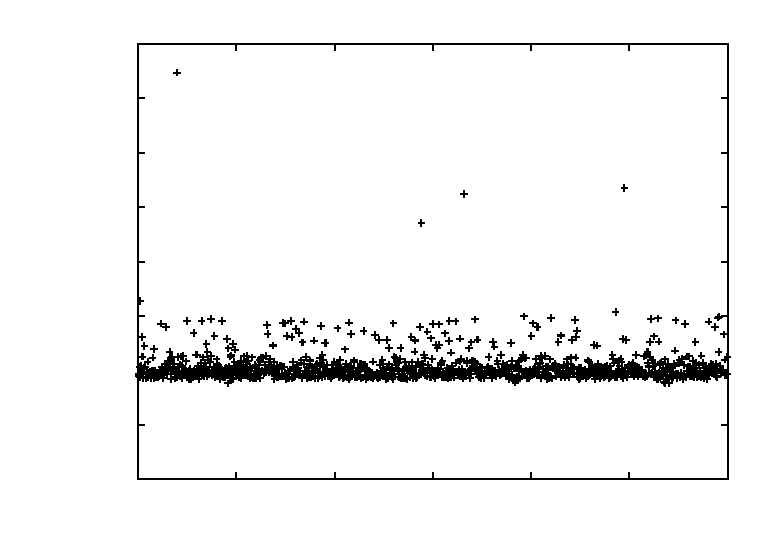
\includegraphics{fig/ker23Tot}}%
    \gplfronttext
  \end{picture}%
\endgroup
}}} \hspace{4pt}%

  \subfloat[\textbf{Linux$^{\mathbf{Prt}}$ - Sem carga} \newline
  \vskip 1mm  {\footnotesize VM: 21.5, DP: 1.7, Min: 20.3, Max: 45.1}]{%
    \label{fig:preSem}%
    {\scalebox{\scaleFact}{% GNUPLOT: LaTeX picture with Postscript
\begingroup
  \makeatletter
  \providecommand\color[2][]{%
    \GenericError{(gnuplot) \space\space\space\@spaces}{%
      Package color not loaded in conjunction with
      terminal option `colourtext'%
    }{See the gnuplot documentation for explanation.%
    }{Either use 'blacktext' in gnuplot or load the package
      color.sty in LaTeX.}%
    \renewcommand\color[2][]{}%
  }%
  \providecommand\includegraphics[2][]{%
    \GenericError{(gnuplot) \space\space\space\@spaces}{%
      Package graphicx or graphics not loaded%
    }{See the gnuplot documentation for explanation.%
    }{The gnuplot epslatex terminal needs graphicx.sty or graphics.sty.}%
    \renewcommand\includegraphics[2][]{}%
  }%
  \providecommand\rotatebox[2]{#2}%
  \@ifundefined{ifGPcolor}{%
    \newif\ifGPcolor
    \GPcolorfalse
  }{}%
  \@ifundefined{ifGPblacktext}{%
    \newif\ifGPblacktext
    \GPblacktextfalse
  }{}%
  % define a \g@addto@macro without @ in the name:
  \let\gplgaddtomacro\g@addto@macro
  % define empty templates for all commands taking text:
  \gdef\gplbacktext{}%
  \gdef\gplfronttext{}%
  \makeatother
  \ifGPblacktext
    % no textcolor at all
    \def\colorrgb#1{}%
    \def\colorgray#1{}%
  \else
    % gray or color?
    \ifGPcolor
      \def\colorrgb#1{\color[rgb]{#1}}%
      \def\colorgray#1{\color[gray]{#1}}%
      \expandafter\def\csname LTw\endcsname{\color{white}}%
      \expandafter\def\csname LTb\endcsname{\color{black}}%
      \expandafter\def\csname LTa\endcsname{\color{black}}%
      \expandafter\def\csname LT0\endcsname{\color[rgb]{1,0,0}}%
      \expandafter\def\csname LT1\endcsname{\color[rgb]{0,1,0}}%
      \expandafter\def\csname LT2\endcsname{\color[rgb]{0,0,1}}%
      \expandafter\def\csname LT3\endcsname{\color[rgb]{1,0,1}}%
      \expandafter\def\csname LT4\endcsname{\color[rgb]{0,1,1}}%
      \expandafter\def\csname LT5\endcsname{\color[rgb]{1,1,0}}%
      \expandafter\def\csname LT6\endcsname{\color[rgb]{0,0,0}}%
      \expandafter\def\csname LT7\endcsname{\color[rgb]{1,0.3,0}}%
      \expandafter\def\csname LT8\endcsname{\color[rgb]{0.5,0.5,0.5}}%
    \else
      % gray
      \def\colorrgb#1{\color{black}}%
      \def\colorgray#1{\color[gray]{#1}}%
      \expandafter\def\csname LTw\endcsname{\color{white}}%
      \expandafter\def\csname LTb\endcsname{\color{black}}%
      \expandafter\def\csname LTa\endcsname{\color{black}}%
      \expandafter\def\csname LT0\endcsname{\color{black}}%
      \expandafter\def\csname LT1\endcsname{\color{black}}%
      \expandafter\def\csname LT2\endcsname{\color{black}}%
      \expandafter\def\csname LT3\endcsname{\color{black}}%
      \expandafter\def\csname LT4\endcsname{\color{black}}%
      \expandafter\def\csname LT5\endcsname{\color{black}}%
      \expandafter\def\csname LT6\endcsname{\color{black}}%
      \expandafter\def\csname LT7\endcsname{\color{black}}%
      \expandafter\def\csname LT8\endcsname{\color{black}}%
    \fi
  \fi
  \setlength{\unitlength}{0.0500bp}%
  \begin{picture}(7200.00,5040.00)%
    \gplgaddtomacro\gplbacktext{%
      \csname LTb\endcsname%
      \put(1034,873){\makebox(0,0)[r]{\strut{}$16.0$}}%
      \put(1034,1430){\makebox(0,0)[r]{\strut{}$18.0$}}%
      \put(1034,1988){\makebox(0,0)[r]{\strut{}$20.0$}}%
      \put(1034,2546){\makebox(0,0)[r]{\strut{}$22.0$}}%
      \put(1034,3103){\makebox(0,0)[r]{\strut{}$24.0$}}%
      \put(1034,3661){\makebox(0,0)[r]{\strut{}$26.0$}}%
      \put(1034,4218){\makebox(0,0)[r]{\strut{}$28.0$}}%
      \put(1034,4776){\makebox(0,0)[r]{\strut{}$30.0$}}%
      \put(1166,374){\makebox(0,0){\strut{}$ 0$}}%
      \put(2109,374){\makebox(0,0){\strut{}$ 10$}}%
      \put(3053,374){\makebox(0,0){\strut{}$ 20$}}%
      \put(3996,374){\makebox(0,0){\strut{}$ 30$}}%
      \put(4939,374){\makebox(0,0){\strut{}$ 40$}}%
      \put(5883,374){\makebox(0,0){\strut{}$ 50$}}%
      \put(6826,374){\makebox(0,0){\strut{}$ 60$}}%
      \put(396,2685){\rotatebox{90}{\makebox(0,0){\strut{}Lat\^encia em $\mu s$}}}%
      \put(3996,110){\makebox(0,0){\strut{}Tempo de observa\c{c}\~ao em $s$}}%
    }%
    \gplgaddtomacro\gplfronttext{%
    }%
    \gplbacktext
    \put(0,0){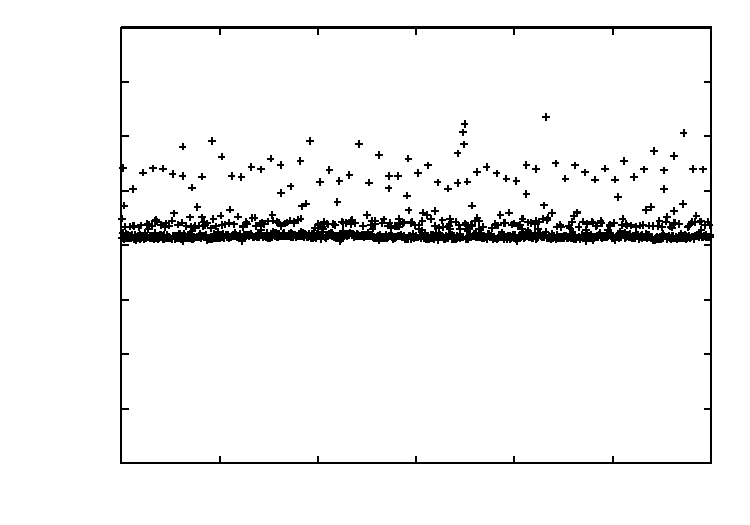
\includegraphics{fig2/preSem}}%
    \gplfronttext
  \end{picture}%
\endgroup
}}} \hspace{4pt}%
  \hspace{\spaceFact}%
  \subfloat[\textbf{Linux$^{\mathbf{Prt}}$ - Com carga} \newline
  \vskip 1mm {\footnotesize VM: 58.5, DP: 26.4, Min: 17.2, Max: 245.9}]{%
    \label{fig:preTot}%
    {\scalebox{\scaleFact}{% GNUPLOT: LaTeX picture with Postscript
\begingroup
  \makeatletter
  \providecommand\color[2][]{%
    \GenericError{(gnuplot) \space\space\space\@spaces}{%
      Package color not loaded in conjunction with
      terminal option `colourtext'%
    }{See the gnuplot documentation for explanation.%
    }{Either use 'blacktext' in gnuplot or load the package
      color.sty in LaTeX.}%
    \renewcommand\color[2][]{}%
  }%
  \providecommand\includegraphics[2][]{%
    \GenericError{(gnuplot) \space\space\space\@spaces}{%
      Package graphicx or graphics not loaded%
    }{See the gnuplot documentation for explanation.%
    }{The gnuplot epslatex terminal needs graphicx.sty or graphics.sty.}%
    \renewcommand\includegraphics[2][]{}%
  }%
  \providecommand\rotatebox[2]{#2}%
  \@ifundefined{ifGPcolor}{%
    \newif\ifGPcolor
    \GPcolorfalse
  }{}%
  \@ifundefined{ifGPblacktext}{%
    \newif\ifGPblacktext
    \GPblacktextfalse
  }{}%
  % define a \g@addto@macro without @ in the name:
  \let\gplgaddtomacro\g@addto@macro
  % define empty templates for all commands taking text:
  \gdef\gplbacktext{}%
  \gdef\gplfronttext{}%
  \makeatother
  \ifGPblacktext
    % no textcolor at all
    \def\colorrgb#1{}%
    \def\colorgray#1{}%
  \else
    % gray or color?
    \ifGPcolor
      \def\colorrgb#1{\color[rgb]{#1}}%
      \def\colorgray#1{\color[gray]{#1}}%
      \expandafter\def\csname LTw\endcsname{\color{white}}%
      \expandafter\def\csname LTb\endcsname{\color{black}}%
      \expandafter\def\csname LTa\endcsname{\color{black}}%
      \expandafter\def\csname LT0\endcsname{\color[rgb]{1,0,0}}%
      \expandafter\def\csname LT1\endcsname{\color[rgb]{0,1,0}}%
      \expandafter\def\csname LT2\endcsname{\color[rgb]{0,0,1}}%
      \expandafter\def\csname LT3\endcsname{\color[rgb]{1,0,1}}%
      \expandafter\def\csname LT4\endcsname{\color[rgb]{0,1,1}}%
      \expandafter\def\csname LT5\endcsname{\color[rgb]{1,1,0}}%
      \expandafter\def\csname LT6\endcsname{\color[rgb]{0,0,0}}%
      \expandafter\def\csname LT7\endcsname{\color[rgb]{1,0.3,0}}%
      \expandafter\def\csname LT8\endcsname{\color[rgb]{0.5,0.5,0.5}}%
    \else
      % gray
      \def\colorrgb#1{\color{black}}%
      \def\colorgray#1{\color[gray]{#1}}%
      \expandafter\def\csname LTw\endcsname{\color{white}}%
      \expandafter\def\csname LTb\endcsname{\color{black}}%
      \expandafter\def\csname LTa\endcsname{\color{black}}%
      \expandafter\def\csname LT0\endcsname{\color{black}}%
      \expandafter\def\csname LT1\endcsname{\color{black}}%
      \expandafter\def\csname LT2\endcsname{\color{black}}%
      \expandafter\def\csname LT3\endcsname{\color{black}}%
      \expandafter\def\csname LT4\endcsname{\color{black}}%
      \expandafter\def\csname LT5\endcsname{\color{black}}%
      \expandafter\def\csname LT6\endcsname{\color{black}}%
      \expandafter\def\csname LT7\endcsname{\color{black}}%
      \expandafter\def\csname LT8\endcsname{\color{black}}%
    \fi
  \fi
  \setlength{\unitlength}{0.0500bp}%
  \begin{picture}(7200.00,5040.00)%
    \gplgaddtomacro\gplbacktext{%
      \csname LTb\endcsname%
      \put(1034,594){\makebox(0,0)[r]{\strut{}$0.0$}}%
      \put(1034,1430){\makebox(0,0)[r]{\strut{}$10.0$}}%
      \put(1034,2267){\makebox(0,0)[r]{\strut{}$20.0$}}%
      \put(1034,3103){\makebox(0,0)[r]{\strut{}$30.0$}}%
      \put(1034,3940){\makebox(0,0)[r]{\strut{}$40.0$}}%
      \put(1034,4776){\makebox(0,0)[r]{\strut{}$50.0$}}%
      \put(1166,374){\makebox(0,0){\strut{}$ 0$}}%
      \put(2109,374){\makebox(0,0){\strut{}$ 10$}}%
      \put(3053,374){\makebox(0,0){\strut{}$ 20$}}%
      \put(3996,374){\makebox(0,0){\strut{}$ 30$}}%
      \put(4939,374){\makebox(0,0){\strut{}$ 40$}}%
      \put(5883,374){\makebox(0,0){\strut{}$ 50$}}%
      \put(6826,374){\makebox(0,0){\strut{}$ 60$}}%
      \put(396,2685){\rotatebox{90}{\makebox(0,0){\strut{}Latency ($\mu s$)}}}%
      \put(3996,110){\makebox(0,0){\strut{}Time ($s$)}}%
    }%
    \gplgaddtomacro\gplfronttext{%
    }%
    \gplbacktext
    \put(0,0){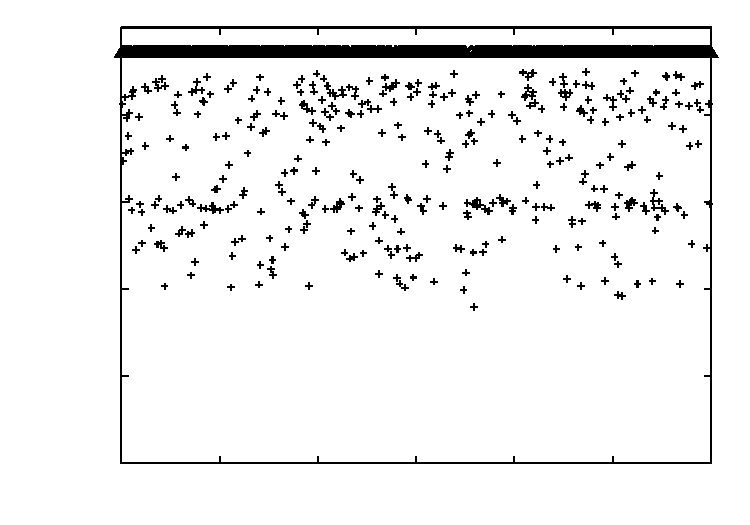
\includegraphics{fig/preTot.pdf}}%
    \gplfronttext
  \end{picture}%
\endgroup
}}} \hspace{4pt}%

  \subfloat[\textbf{Linux$^{\mathbf{Rtai}}$ - Sem carga} \newline
  \vskip 1mm {\footnotesize VM: 8.7, DP: 0.1, Min: 8.8, Max: 10.7}]{%
    \label{fig:rtaiSem}%
    {\scalebox{\scaleFact}{% GNUPLOT: LaTeX picture with Postscript
\begingroup
  \makeatletter
  \providecommand\color[2][]{%
    \GenericError{(gnuplot) \space\space\space\@spaces}{%
      Package color not loaded in conjunction with
      terminal option `colourtext'%
    }{See the gnuplot documentation for explanation.%
    }{Either use 'blacktext' in gnuplot or load the package
      color.sty in LaTeX.}%
    \renewcommand\color[2][]{}%
  }%
  \providecommand\includegraphics[2][]{%
    \GenericError{(gnuplot) \space\space\space\@spaces}{%
      Package graphicx or graphics not loaded%
    }{See the gnuplot documentation for explanation.%
    }{The gnuplot epslatex terminal needs graphicx.sty or graphics.sty.}%
    \renewcommand\includegraphics[2][]{}%
  }%
  \providecommand\rotatebox[2]{#2}%
  \@ifundefined{ifGPcolor}{%
    \newif\ifGPcolor
    \GPcolorfalse
  }{}%
  \@ifundefined{ifGPblacktext}{%
    \newif\ifGPblacktext
    \GPblacktexttrue
  }{}%
  % define a \g@addto@macro without @ in the name:
  \let\gplgaddtomacro\g@addto@macro
  % define empty templates for all commands taking text:
  \gdef\gplbacktext{}%
  \gdef\gplfronttext{}%
  \makeatother
  \ifGPblacktext
    % no textcolor at all
    \def\colorrgb#1{}%
    \def\colorgray#1{}%
  \else
    % gray or color?
    \ifGPcolor
      \def\colorrgb#1{\color[rgb]{#1}}%
      \def\colorgray#1{\color[gray]{#1}}%
      \expandafter\def\csname LTw\endcsname{\color{white}}%
      \expandafter\def\csname LTb\endcsname{\color{black}}%
      \expandafter\def\csname LTa\endcsname{\color{black}}%
      \expandafter\def\csname LT0\endcsname{\color[rgb]{1,0,0}}%
      \expandafter\def\csname LT1\endcsname{\color[rgb]{0,1,0}}%
      \expandafter\def\csname LT2\endcsname{\color[rgb]{0,0,1}}%
      \expandafter\def\csname LT3\endcsname{\color[rgb]{1,0,1}}%
      \expandafter\def\csname LT4\endcsname{\color[rgb]{0,1,1}}%
      \expandafter\def\csname LT5\endcsname{\color[rgb]{1,1,0}}%
      \expandafter\def\csname LT6\endcsname{\color[rgb]{0,0,0}}%
      \expandafter\def\csname LT7\endcsname{\color[rgb]{1,0.3,0}}%
      \expandafter\def\csname LT8\endcsname{\color[rgb]{0.5,0.5,0.5}}%
    \else
      % gray
      \def\colorrgb#1{\color{black}}%
      \def\colorgray#1{\color[gray]{#1}}%
      \expandafter\def\csname LTw\endcsname{\color{white}}%
      \expandafter\def\csname LTb\endcsname{\color{black}}%
      \expandafter\def\csname LTa\endcsname{\color{black}}%
      \expandafter\def\csname LT0\endcsname{\color{black}}%
      \expandafter\def\csname LT1\endcsname{\color{black}}%
      \expandafter\def\csname LT2\endcsname{\color{black}}%
      \expandafter\def\csname LT3\endcsname{\color{black}}%
      \expandafter\def\csname LT4\endcsname{\color{black}}%
      \expandafter\def\csname LT5\endcsname{\color{black}}%
      \expandafter\def\csname LT6\endcsname{\color{black}}%
      \expandafter\def\csname LT7\endcsname{\color{black}}%
      \expandafter\def\csname LT8\endcsname{\color{black}}%
    \fi
  \fi
  \setlength{\unitlength}{0.0500bp}%
  \begin{picture}(7200.00,5040.00)%
    \gplgaddtomacro\gplbacktext{%
      \csname LTb\endcsname%
      \put(1254,660){\makebox(0,0)[r]{\strut{}$5.0$}}%
      \put(1254,1346){\makebox(0,0)[r]{\strut{}$10.0$}}%
      \put(1254,2032){\makebox(0,0)[r]{\strut{}$15.0$}}%
      \put(1254,2718){\makebox(0,0)[r]{\strut{}$20.0$}}%
      \put(1254,3404){\makebox(0,0)[r]{\strut{}$25.0$}}%
      \put(1254,4090){\makebox(0,0)[r]{\strut{}$30.0$}}%
      \put(1254,4776){\makebox(0,0)[r]{\strut{}$35.0$}}%
      \put(1386,440){\makebox(0,0){\strut{}$ 0$}}%
      \put(2293,440){\makebox(0,0){\strut{}$ 10$}}%
      \put(3199,440){\makebox(0,0){\strut{}$ 20$}}%
      \put(4106,440){\makebox(0,0){\strut{}$ 30$}}%
      \put(5013,440){\makebox(0,0){\strut{}$ 40$}}%
      \put(5919,440){\makebox(0,0){\strut{}$ 50$}}%
      \put(6826,440){\makebox(0,0){\strut{}$ 60$}}%
      \put(220,2718){\rotatebox{90}{\makebox(0,0){\strut{}Lat\^encia em $\mu s$}}}%
      \put(4106,110){\makebox(0,0){\strut{}Tempo de observa\c{c}\~ao em $s$}}%
    }%
    \gplgaddtomacro\gplfronttext{%
    }%
    \gplbacktext
    \put(0,0){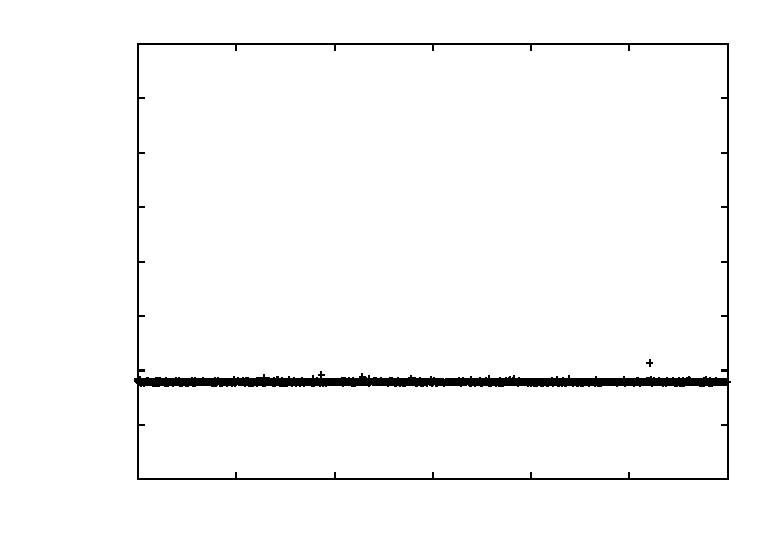
\includegraphics{fig/rtaiSem}}%
    \gplfronttext
  \end{picture}%
\endgroup
}}} \hspace{4pt}%
  \hspace{\spaceFact}%
  \subfloat[\textbf{Linux$^{\mathbf{Rtai}}$ - Com carga} \newline
  \vskip 1mm  {\footnotesize VM: 10.0, DP: 0.8, Min: 8.8, Max: 20.8}]{%
    \label{fig:rtaiTot}%
    {\scalebox{\scaleFact}{% GNUPLOT: LaTeX picture with Postscript
\begingroup
  \makeatletter
  \providecommand\color[2][]{%
    \GenericError{(gnuplot) \space\space\space\@spaces}{%
      Package color not loaded in conjunction with
      terminal option `colourtext'%
    }{See the gnuplot documentation for explanation.%
    }{Either use 'blacktext' in gnuplot or load the package
      color.sty in LaTeX.}%
    \renewcommand\color[2][]{}%
  }%
  \providecommand\includegraphics[2][]{%
    \GenericError{(gnuplot) \space\space\space\@spaces}{%
      Package graphicx or graphics not loaded%
    }{See the gnuplot documentation for explanation.%
    }{The gnuplot epslatex terminal needs graphicx.sty or graphics.sty.}%
    \renewcommand\includegraphics[2][]{}%
  }%
  \providecommand\rotatebox[2]{#2}%
  \@ifundefined{ifGPcolor}{%
    \newif\ifGPcolor
    \GPcolorfalse
  }{}%
  \@ifundefined{ifGPblacktext}{%
    \newif\ifGPblacktext
    \GPblacktextfalse
  }{}%
  % define a \g@addto@macro without @ in the name:
  \let\gplgaddtomacro\g@addto@macro
  % define empty templates for all commands taking text:
  \gdef\gplbacktext{}%
  \gdef\gplfronttext{}%
  \makeatother
  \ifGPblacktext
    % no textcolor at all
    \def\colorrgb#1{}%
    \def\colorgray#1{}%
  \else
    % gray or color?
    \ifGPcolor
      \def\colorrgb#1{\color[rgb]{#1}}%
      \def\colorgray#1{\color[gray]{#1}}%
      \expandafter\def\csname LTw\endcsname{\color{white}}%
      \expandafter\def\csname LTb\endcsname{\color{black}}%
      \expandafter\def\csname LTa\endcsname{\color{black}}%
      \expandafter\def\csname LT0\endcsname{\color[rgb]{1,0,0}}%
      \expandafter\def\csname LT1\endcsname{\color[rgb]{0,1,0}}%
      \expandafter\def\csname LT2\endcsname{\color[rgb]{0,0,1}}%
      \expandafter\def\csname LT3\endcsname{\color[rgb]{1,0,1}}%
      \expandafter\def\csname LT4\endcsname{\color[rgb]{0,1,1}}%
      \expandafter\def\csname LT5\endcsname{\color[rgb]{1,1,0}}%
      \expandafter\def\csname LT6\endcsname{\color[rgb]{0,0,0}}%
      \expandafter\def\csname LT7\endcsname{\color[rgb]{1,0.3,0}}%
      \expandafter\def\csname LT8\endcsname{\color[rgb]{0.5,0.5,0.5}}%
    \else
      % gray
      \def\colorrgb#1{\color{black}}%
      \def\colorgray#1{\color[gray]{#1}}%
      \expandafter\def\csname LTw\endcsname{\color{white}}%
      \expandafter\def\csname LTb\endcsname{\color{black}}%
      \expandafter\def\csname LTa\endcsname{\color{black}}%
      \expandafter\def\csname LT0\endcsname{\color{black}}%
      \expandafter\def\csname LT1\endcsname{\color{black}}%
      \expandafter\def\csname LT2\endcsname{\color{black}}%
      \expandafter\def\csname LT3\endcsname{\color{black}}%
      \expandafter\def\csname LT4\endcsname{\color{black}}%
      \expandafter\def\csname LT5\endcsname{\color{black}}%
      \expandafter\def\csname LT6\endcsname{\color{black}}%
      \expandafter\def\csname LT7\endcsname{\color{black}}%
      \expandafter\def\csname LT8\endcsname{\color{black}}%
    \fi
  \fi
  \setlength{\unitlength}{0.0500bp}%
  \begin{picture}(7200.00,5040.00)%
    \gplgaddtomacro\gplbacktext{%
      \csname LTb\endcsname%
      \put(1034,594){\makebox(0,0)[r]{\strut{}$0.0$}}%
      \put(1034,1117){\makebox(0,0)[r]{\strut{}$5.0$}}%
      \put(1034,1640){\makebox(0,0)[r]{\strut{}$10.0$}}%
      \put(1034,2162){\makebox(0,0)[r]{\strut{}$15.0$}}%
      \put(1034,2685){\makebox(0,0)[r]{\strut{}$20.0$}}%
      \put(1034,3208){\makebox(0,0)[r]{\strut{}$25.0$}}%
      \put(1034,3731){\makebox(0,0)[r]{\strut{}$30.0$}}%
      \put(1034,4253){\makebox(0,0)[r]{\strut{}$35.0$}}%
      \put(1034,4776){\makebox(0,0)[r]{\strut{}$40.0$}}%
      \put(1166,374){\makebox(0,0){\strut{}$ 0$}}%
      \put(2109,374){\makebox(0,0){\strut{}$ 10$}}%
      \put(3053,374){\makebox(0,0){\strut{}$ 20$}}%
      \put(3996,374){\makebox(0,0){\strut{}$ 30$}}%
      \put(4939,374){\makebox(0,0){\strut{}$ 40$}}%
      \put(5883,374){\makebox(0,0){\strut{}$ 50$}}%
      \put(6826,374){\makebox(0,0){\strut{}$ 60$}}%
      \put(396,2685){\rotatebox{90}{\makebox(0,0){\strut{}Lat\^encia em $\mu s$}}}%
      \put(3996,110){\makebox(0,0){\strut{}Tempo de observa\c{c}\~ao em $s$}}%
    }%
    \gplgaddtomacro\gplfronttext{%
    }%
    \gplbacktext
    \put(0,0){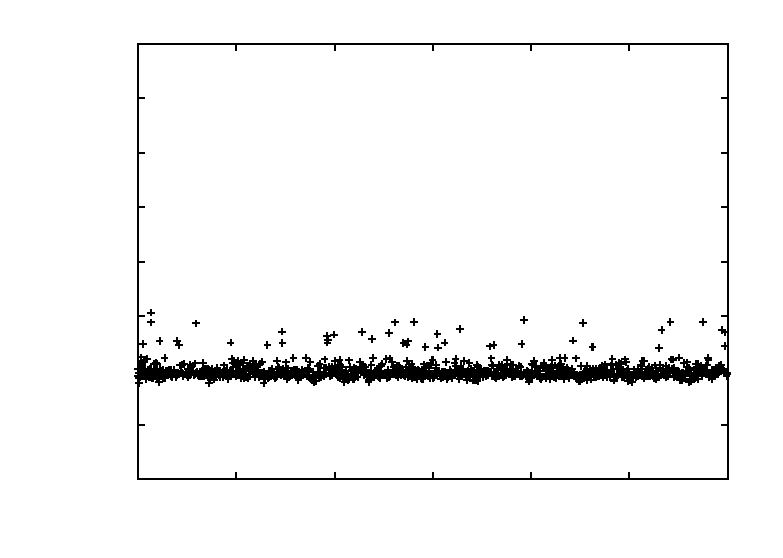
\includegraphics{fig/rtaiTot}}%
    \gplfronttext
  \end{picture}%
\endgroup
}}} \hspace{4pt}%

  \subfloat[\textbf{Linux$^{\mathbf{Xen}}$ - Sem carga} \newline
  \vskip 1mm {\footnotesize VM: 9.0, DP: 0.1, Min: 8.8, Max: 11.1}]{%
    \label{fig:xenSem}%
    {\scalebox{\scaleFact}{% GNUPLOT: LaTeX picture with Postscript
\begingroup
  \makeatletter
  \providecommand\color[2][]{%
    \GenericError{(gnuplot) \space\space\space\@spaces}{%
      Package color not loaded in conjunction with
      terminal option `colourtext'%
    }{See the gnuplot documentation for explanation.%
    }{Either use 'blacktext' in gnuplot or load the package
      color.sty in LaTeX.}%
    \renewcommand\color[2][]{}%
  }%
  \providecommand\includegraphics[2][]{%
    \GenericError{(gnuplot) \space\space\space\@spaces}{%
      Package graphicx or graphics not loaded%
    }{See the gnuplot documentation for explanation.%
    }{The gnuplot epslatex terminal needs graphicx.sty or graphics.sty.}%
    \renewcommand\includegraphics[2][]{}%
  }%
  \providecommand\rotatebox[2]{#2}%
  \@ifundefined{ifGPcolor}{%
    \newif\ifGPcolor
    \GPcolorfalse
  }{}%
  \@ifundefined{ifGPblacktext}{%
    \newif\ifGPblacktext
    \GPblacktexttrue
  }{}%
  % define a \g@addto@macro without @ in the name:
  \let\gplgaddtomacro\g@addto@macro
  % define empty templates for all commands taking text:
  \gdef\gplbacktext{}%
  \gdef\gplfronttext{}%
  \makeatother
  \ifGPblacktext
    % no textcolor at all
    \def\colorrgb#1{}%
    \def\colorgray#1{}%
  \else
    % gray or color?
    \ifGPcolor
      \def\colorrgb#1{\color[rgb]{#1}}%
      \def\colorgray#1{\color[gray]{#1}}%
      \expandafter\def\csname LTw\endcsname{\color{white}}%
      \expandafter\def\csname LTb\endcsname{\color{black}}%
      \expandafter\def\csname LTa\endcsname{\color{black}}%
      \expandafter\def\csname LT0\endcsname{\color[rgb]{1,0,0}}%
      \expandafter\def\csname LT1\endcsname{\color[rgb]{0,1,0}}%
      \expandafter\def\csname LT2\endcsname{\color[rgb]{0,0,1}}%
      \expandafter\def\csname LT3\endcsname{\color[rgb]{1,0,1}}%
      \expandafter\def\csname LT4\endcsname{\color[rgb]{0,1,1}}%
      \expandafter\def\csname LT5\endcsname{\color[rgb]{1,1,0}}%
      \expandafter\def\csname LT6\endcsname{\color[rgb]{0,0,0}}%
      \expandafter\def\csname LT7\endcsname{\color[rgb]{1,0.3,0}}%
      \expandafter\def\csname LT8\endcsname{\color[rgb]{0.5,0.5,0.5}}%
    \else
      % gray
      \def\colorrgb#1{\color{black}}%
      \def\colorgray#1{\color[gray]{#1}}%
      \expandafter\def\csname LTw\endcsname{\color{white}}%
      \expandafter\def\csname LTb\endcsname{\color{black}}%
      \expandafter\def\csname LTa\endcsname{\color{black}}%
      \expandafter\def\csname LT0\endcsname{\color{black}}%
      \expandafter\def\csname LT1\endcsname{\color{black}}%
      \expandafter\def\csname LT2\endcsname{\color{black}}%
      \expandafter\def\csname LT3\endcsname{\color{black}}%
      \expandafter\def\csname LT4\endcsname{\color{black}}%
      \expandafter\def\csname LT5\endcsname{\color{black}}%
      \expandafter\def\csname LT6\endcsname{\color{black}}%
      \expandafter\def\csname LT7\endcsname{\color{black}}%
      \expandafter\def\csname LT8\endcsname{\color{black}}%
    \fi
  \fi
  \setlength{\unitlength}{0.0500bp}%
  \begin{picture}(7200.00,5040.00)%
    \gplgaddtomacro\gplbacktext{%
      \csname LTb\endcsname%
      \put(1386,660){\makebox(0,0)[r]{\strut{}$0.0$}}%
      \put(1386,1483){\makebox(0,0)[r]{\strut{}$20.0$}}%
      \put(1386,2306){\makebox(0,0)[r]{\strut{}$40.0$}}%
      \put(1386,3130){\makebox(0,0)[r]{\strut{}$60.0$}}%
      \put(1386,3953){\makebox(0,0)[r]{\strut{}$80.0$}}%
      \put(1386,4776){\makebox(0,0)[r]{\strut{}$100.0$}}%
      \put(1518,440){\makebox(0,0){\strut{}$ 0$}}%
      \put(2403,440){\makebox(0,0){\strut{}$ 10$}}%
      \put(3287,440){\makebox(0,0){\strut{}$ 20$}}%
      \put(4172,440){\makebox(0,0){\strut{}$ 30$}}%
      \put(5057,440){\makebox(0,0){\strut{}$ 40$}}%
      \put(5941,440){\makebox(0,0){\strut{}$ 50$}}%
      \put(6826,440){\makebox(0,0){\strut{}$ 60$}}%
      \put(220,2718){\rotatebox{90}{\makebox(0,0){\strut{}Lat\^encia em $\mu s$}}}%
      \put(4172,110){\makebox(0,0){\strut{}Tempo de observa\c{c}\~ao em $s$}}%
    }%
    \gplgaddtomacro\gplfronttext{%
    }%
    \gplbacktext
    \put(0,0){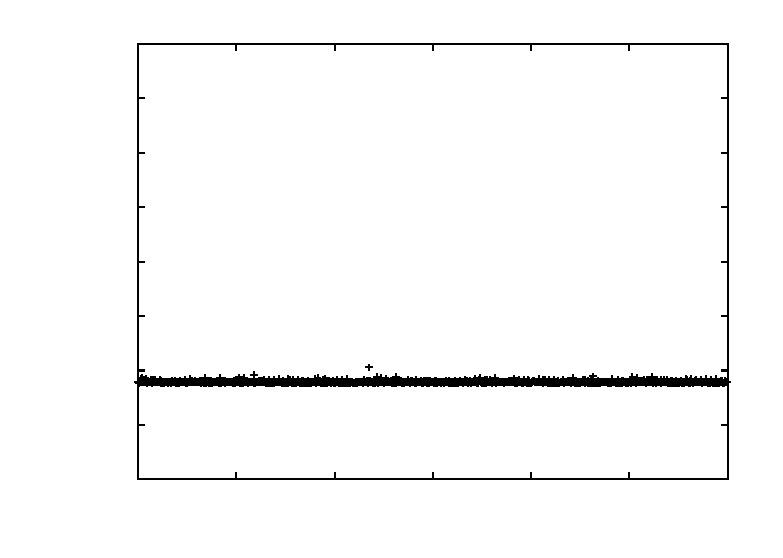
\includegraphics{fig/xenSem}}%
    \gplfronttext
  \end{picture}%
\endgroup
}}} \hspace{4pt}%
  \hspace{\spaceFact}%
  \subfloat[\textbf{Linux$^{\mathbf{Xen}}$ - Com carga} \newline
  \vskip 1mm {\footnotesize VM: 10.4, DP: 0.7, Min: 8.9, Max: 20.8}]{%
    \label{fig:xenTot}%
    {\scalebox{\scaleFact}{% GNUPLOT: LaTeX picture with Postscript
\begingroup
  \makeatletter
  \providecommand\color[2][]{%
    \GenericError{(gnuplot) \space\space\space\@spaces}{%
      Package color not loaded in conjunction with
      terminal option `colourtext'%
    }{See the gnuplot documentation for explanation.%
    }{Either use 'blacktext' in gnuplot or load the package
      color.sty in LaTeX.}%
    \renewcommand\color[2][]{}%
  }%
  \providecommand\includegraphics[2][]{%
    \GenericError{(gnuplot) \space\space\space\@spaces}{%
      Package graphicx or graphics not loaded%
    }{See the gnuplot documentation for explanation.%
    }{The gnuplot epslatex terminal needs graphicx.sty or graphics.sty.}%
    \renewcommand\includegraphics[2][]{}%
  }%
  \providecommand\rotatebox[2]{#2}%
  \@ifundefined{ifGPcolor}{%
    \newif\ifGPcolor
    \GPcolorfalse
  }{}%
  \@ifundefined{ifGPblacktext}{%
    \newif\ifGPblacktext
    \GPblacktextfalse
  }{}%
  % define a \g@addto@macro without @ in the name:
  \let\gplgaddtomacro\g@addto@macro
  % define empty templates for all commands taking text:
  \gdef\gplbacktext{}%
  \gdef\gplfronttext{}%
  \makeatother
  \ifGPblacktext
    % no textcolor at all
    \def\colorrgb#1{}%
    \def\colorgray#1{}%
  \else
    % gray or color?
    \ifGPcolor
      \def\colorrgb#1{\color[rgb]{#1}}%
      \def\colorgray#1{\color[gray]{#1}}%
      \expandafter\def\csname LTw\endcsname{\color{white}}%
      \expandafter\def\csname LTb\endcsname{\color{black}}%
      \expandafter\def\csname LTa\endcsname{\color{black}}%
      \expandafter\def\csname LT0\endcsname{\color[rgb]{1,0,0}}%
      \expandafter\def\csname LT1\endcsname{\color[rgb]{0,1,0}}%
      \expandafter\def\csname LT2\endcsname{\color[rgb]{0,0,1}}%
      \expandafter\def\csname LT3\endcsname{\color[rgb]{1,0,1}}%
      \expandafter\def\csname LT4\endcsname{\color[rgb]{0,1,1}}%
      \expandafter\def\csname LT5\endcsname{\color[rgb]{1,1,0}}%
      \expandafter\def\csname LT6\endcsname{\color[rgb]{0,0,0}}%
      \expandafter\def\csname LT7\endcsname{\color[rgb]{1,0.3,0}}%
      \expandafter\def\csname LT8\endcsname{\color[rgb]{0.5,0.5,0.5}}%
    \else
      % gray
      \def\colorrgb#1{\color{black}}%
      \def\colorgray#1{\color[gray]{#1}}%
      \expandafter\def\csname LTw\endcsname{\color{white}}%
      \expandafter\def\csname LTb\endcsname{\color{black}}%
      \expandafter\def\csname LTa\endcsname{\color{black}}%
      \expandafter\def\csname LT0\endcsname{\color{black}}%
      \expandafter\def\csname LT1\endcsname{\color{black}}%
      \expandafter\def\csname LT2\endcsname{\color{black}}%
      \expandafter\def\csname LT3\endcsname{\color{black}}%
      \expandafter\def\csname LT4\endcsname{\color{black}}%
      \expandafter\def\csname LT5\endcsname{\color{black}}%
      \expandafter\def\csname LT6\endcsname{\color{black}}%
      \expandafter\def\csname LT7\endcsname{\color{black}}%
      \expandafter\def\csname LT8\endcsname{\color{black}}%
    \fi
  \fi
  \setlength{\unitlength}{0.0500bp}%
  \begin{picture}(7200.00,5040.00)%
    \gplgaddtomacro\gplbacktext{%
      \csname LTb\endcsname%
      \put(1254,660){\makebox(0,0)[r]{\strut{}$8.0$}}%
      \put(1254,1117){\makebox(0,0)[r]{\strut{}$9.0$}}%
      \put(1254,1575){\makebox(0,0)[r]{\strut{}$10.0$}}%
      \put(1254,2032){\makebox(0,0)[r]{\strut{}$11.0$}}%
      \put(1254,2489){\makebox(0,0)[r]{\strut{}$12.0$}}%
      \put(1254,2947){\makebox(0,0)[r]{\strut{}$13.0$}}%
      \put(1254,3404){\makebox(0,0)[r]{\strut{}$14.0$}}%
      \put(1254,3861){\makebox(0,0)[r]{\strut{}$15.0$}}%
      \put(1254,4319){\makebox(0,0)[r]{\strut{}$16.0$}}%
      \put(1254,4776){\makebox(0,0)[r]{\strut{}$17.0$}}%
      \put(1386,440){\makebox(0,0){\strut{}$ 0$}}%
      \put(2293,440){\makebox(0,0){\strut{}$ 10$}}%
      \put(3199,440){\makebox(0,0){\strut{}$ 20$}}%
      \put(4106,440){\makebox(0,0){\strut{}$ 30$}}%
      \put(5013,440){\makebox(0,0){\strut{}$ 40$}}%
      \put(5919,440){\makebox(0,0){\strut{}$ 50$}}%
      \put(6826,440){\makebox(0,0){\strut{}$ 60$}}%
      \put(220,2718){\rotatebox{90}{\makebox(0,0){\strut{}Lat\^encia em $\mu s$}}}%
      \put(4106,110){\makebox(0,0){\strut{}Tempo de observa\c{c}\~ao em $s$}}%
    }%
    \gplgaddtomacro\gplfronttext{%
    }%
    \gplbacktext
    \put(0,0){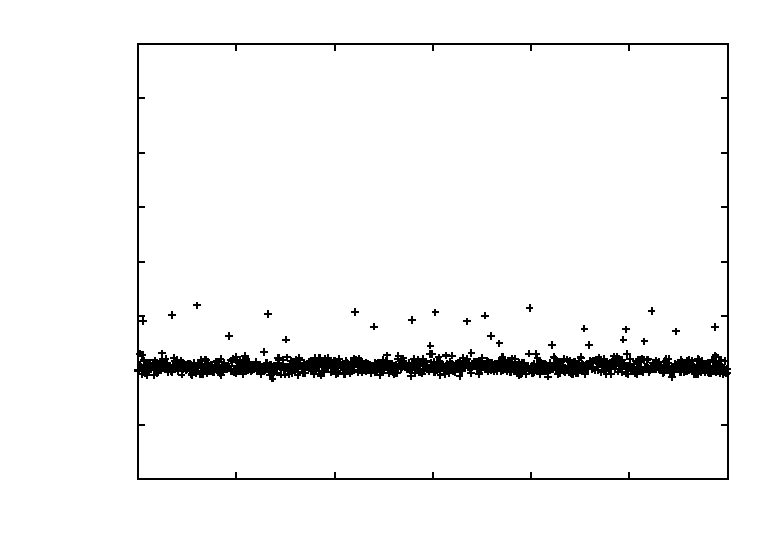
\includegraphics{fig/xenTot}}%
    \gplfronttext
  \end{picture}%
\endgroup
}}} \hspace{4pt}%

  \caption[Lat�ncias de interrup��o]{Lat�ncia de interrup��o com
    freq��ncia de escrita na PP de $20 Hz$.}
  \label{fig:latIrq}%
\end{figure}


A figura \ref{fig:latIrq} apresenta as lat�ncias de interrup��o medidas, com e sem
estresse do sistema.  Como pode ser observado, sem carga, o Linux$^{\mathbf{Std}}$,
Linux$^{\mathbf{Rtai}}$ e Linux$^{\mathbf{Xen}}$ t�m comportamentos parecidos. Com
carga, observa-se uma varia��o significativa do Linux$^{\mathbf{Std}}$, como
esperado.

Com rela��o ao Linux$^{\mathbf{Prt}}$, dois resultados chamam aten��o.  Primeiro, o
comportamento do sistema sem carga exibe lat�ncias da ordem de $20\mu s$. Isto �
causado pela implementa��o dos \ing{threads} de interrup��o vista na se��o
\ref{sec:preemptRT}.  Segundo, contradizendo as expectativas, a aplica��o do
estresse teve um impacto significativo, provocando uma alta variabilidade das
lat�ncias. De fato, entre o instante no qual o tratador $T_{PP}$ acorda o
\ing{thread} de interrup��o e o instante no qual este \ing{thread} acorda
efetivamente, uma ou v�rias interrup��es podem ocorrer.  Neste caso, a execu��o dos
tratadores associados pode provocar o atraso da execu��o de $T_{PP}$.

Para cancelar esta variabilidade indesej�vel, � poss�vel usar o
Linux$^{\mathbf{Prt}}$ sem utilizar a implementa��o de \ing{threads}
de interrup��o.  Para tanto, usa-se a op��o \cod{IRQF\_NODELAY} na
requisi��o da linha de interrup��o. Utilizando esta op��o na
requisi��o da linha de interrup��o da porta paralela, o comportamento
do Linux$^{\mathbf{Prt}}$ passa a ser semelhante ao
Linux$^{\mathbf{Std}}$.

%\pagebreak
\subsubsection{Lat�ncia de ativa��o}

A figura \ref{fig:latAtiv} apresenta os resultados para as lat�ncias de ativa��o sem
estresse e com estresse do processador.  Como pode ser observado, o comportamento de
Linux$^{\mathbf{Std}}$ � inadequado para atender os requisitos de tempo real.
Linux$^{\mathbf{Prt}}$, Linux$^{\mathbf{Rtai}}$ e Linux$^{\mathbf{Xen}}$, por outro
lado, apresentam valores de lat�ncias dentro dos padr�es esperados.  Vale a pena
notar o comportamento destes sistemas com carga.  Constata-se que o valor m�dio
encontrado para Linux$^{\mathbf{Xen}}$ ($8,7\mu s$) � superior ao do
Linux$^{\mathbf{Prt}}$ ($3,8\mu s$) e ao Linux$^{\mathbf{Rtai}}$ ($4,4\mu s$). No
entanto, o desvio padr�o de Linux$^{\mathbf{Xen}}$ � significativamente menor que
este de Linux$^{\mathbf{Prt}}$, caracter�stica desej�vel para sistemas de tempo real
cr�ticos.  Por outro lado, acredita-se que o fato de Linux$^{\mathbf{Xen}}$ ter um
valor m�dio superior ao Linux$^{\mathbf{Rtai}}$ � devido � sobrecarga introduzida
pelo projeto Xenomai para poder oferecer uma interface dispon�vel em modo usu�rio.


\begin{figure}%
  \centering

  \subfloat[\textbf{Linux$^{\mathbf{Std}}$ - Sem carga} \newline
  \vskip 1mm {\footnotesize VM:     4.6, DP:     0.4,  Min:     4.4, Max:    16.2}]{%
    \label{fig:ker23SemSched}%
    {\scalebox{\scaleFact}{% GNUPLOT: LaTeX picture with Postscript
\begingroup
  \makeatletter
  \providecommand\color[2][]{%
    \GenericError{(gnuplot) \space\space\space\@spaces}{%
      Package color not loaded in conjunction with
      terminal option `colourtext'%
    }{See the gnuplot documentation for explanation.%
    }{Either use 'blacktext' in gnuplot or load the package
      color.sty in LaTeX.}%
    \renewcommand\color[2][]{}%
  }%
  \providecommand\includegraphics[2][]{%
    \GenericError{(gnuplot) \space\space\space\@spaces}{%
      Package graphicx or graphics not loaded%
    }{See the gnuplot documentation for explanation.%
    }{The gnuplot epslatex terminal needs graphicx.sty or graphics.sty.}%
    \renewcommand\includegraphics[2][]{}%
  }%
  \providecommand\rotatebox[2]{#2}%
  \@ifundefined{ifGPcolor}{%
    \newif\ifGPcolor
    \GPcolorfalse
  }{}%
  \@ifundefined{ifGPblacktext}{%
    \newif\ifGPblacktext
    \GPblacktextfalse
  }{}%
  % define a \g@addto@macro without @ in the name:
  \let\gplgaddtomacro\g@addto@macro
  % define empty templates for all commands taking text:
  \gdef\gplbacktext{}%
  \gdef\gplfronttext{}%
  \makeatother
  \ifGPblacktext
    % no textcolor at all
    \def\colorrgb#1{}%
    \def\colorgray#1{}%
  \else
    % gray or color?
    \ifGPcolor
      \def\colorrgb#1{\color[rgb]{#1}}%
      \def\colorgray#1{\color[gray]{#1}}%
      \expandafter\def\csname LTw\endcsname{\color{white}}%
      \expandafter\def\csname LTb\endcsname{\color{black}}%
      \expandafter\def\csname LTa\endcsname{\color{black}}%
      \expandafter\def\csname LT0\endcsname{\color[rgb]{1,0,0}}%
      \expandafter\def\csname LT1\endcsname{\color[rgb]{0,1,0}}%
      \expandafter\def\csname LT2\endcsname{\color[rgb]{0,0,1}}%
      \expandafter\def\csname LT3\endcsname{\color[rgb]{1,0,1}}%
      \expandafter\def\csname LT4\endcsname{\color[rgb]{0,1,1}}%
      \expandafter\def\csname LT5\endcsname{\color[rgb]{1,1,0}}%
      \expandafter\def\csname LT6\endcsname{\color[rgb]{0,0,0}}%
      \expandafter\def\csname LT7\endcsname{\color[rgb]{1,0.3,0}}%
      \expandafter\def\csname LT8\endcsname{\color[rgb]{0.5,0.5,0.5}}%
    \else
      % gray
      \def\colorrgb#1{\color{black}}%
      \def\colorgray#1{\color[gray]{#1}}%
      \expandafter\def\csname LTw\endcsname{\color{white}}%
      \expandafter\def\csname LTb\endcsname{\color{black}}%
      \expandafter\def\csname LTa\endcsname{\color{black}}%
      \expandafter\def\csname LT0\endcsname{\color{black}}%
      \expandafter\def\csname LT1\endcsname{\color{black}}%
      \expandafter\def\csname LT2\endcsname{\color{black}}%
      \expandafter\def\csname LT3\endcsname{\color{black}}%
      \expandafter\def\csname LT4\endcsname{\color{black}}%
      \expandafter\def\csname LT5\endcsname{\color{black}}%
      \expandafter\def\csname LT6\endcsname{\color{black}}%
      \expandafter\def\csname LT7\endcsname{\color{black}}%
      \expandafter\def\csname LT8\endcsname{\color{black}}%
    \fi
  \fi
  \setlength{\unitlength}{0.0500bp}%
  \begin{picture}(7200.00,5040.00)%
    \gplgaddtomacro\gplbacktext{%
      \csname LTb\endcsname%
      \put(1034,594){\makebox(0,0)[r]{\strut{}$0.0$}}%
      \put(1034,1640){\makebox(0,0)[r]{\strut{}$5.0$}}%
      \put(1034,2685){\makebox(0,0)[r]{\strut{}$10.0$}}%
      \put(1034,3731){\makebox(0,0)[r]{\strut{}$15.0$}}%
      \put(1034,4776){\makebox(0,0)[r]{\strut{}$20.0$}}%
      \put(1166,374){\makebox(0,0){\strut{}$ 0$}}%
      \put(2109,374){\makebox(0,0){\strut{}$ 10$}}%
      \put(3053,374){\makebox(0,0){\strut{}$ 20$}}%
      \put(3996,374){\makebox(0,0){\strut{}$ 30$}}%
      \put(4939,374){\makebox(0,0){\strut{}$ 40$}}%
      \put(5883,374){\makebox(0,0){\strut{}$ 50$}}%
      \put(6826,374){\makebox(0,0){\strut{}$ 60$}}%
      \put(396,2685){\rotatebox{90}{\makebox(0,0){\strut{}Lat\^encia em $\mu s$}}}%
      \put(3996,110){\makebox(0,0){\strut{}Tempo de observa\c{c}\~ao em $s$}}%
    }%
    \gplgaddtomacro\gplfronttext{%
    }%
    \gplbacktext
    \put(0,0){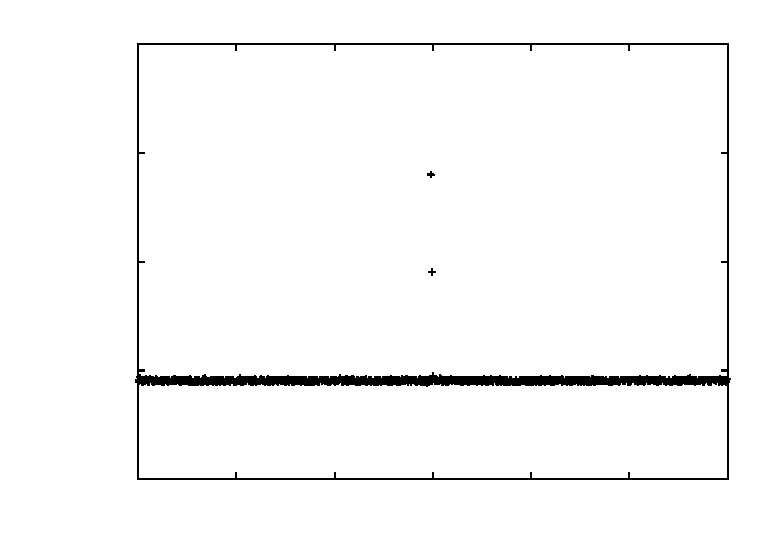
\includegraphics{fig/ker23SemSched}}%
    \gplfronttext
  \end{picture}%
\endgroup
}}}
  \hspace{\spaceFact}%
  \subfloat[\textbf{Linux$^{\mathbf{Std}}$ - Com carga}\newline
  \vskip 1mm {\footnotesize VM:    37.3, DP:    48.2,  Min:     4.6, Max:   617.5}]{%
    \label{fig:ker23TotSched}%
    {\scalebox{\scaleFact}{% GNUPLOT: LaTeX picture with Postscript
\begingroup
  \makeatletter
  \providecommand\color[2][]{%
    \GenericError{(gnuplot) \space\space\space\@spaces}{%
      Package color not loaded in conjunction with
      terminal option `colourtext'%
    }{See the gnuplot documentation for explanation.%
    }{Either use 'blacktext' in gnuplot or load the package
      color.sty in LaTeX.}%
    \renewcommand\color[2][]{}%
  }%
  \providecommand\includegraphics[2][]{%
    \GenericError{(gnuplot) \space\space\space\@spaces}{%
      Package graphicx or graphics not loaded%
    }{See the gnuplot documentation for explanation.%
    }{The gnuplot epslatex terminal needs graphicx.sty or graphics.sty.}%
    \renewcommand\includegraphics[2][]{}%
  }%
  \providecommand\rotatebox[2]{#2}%
  \@ifundefined{ifGPcolor}{%
    \newif\ifGPcolor
    \GPcolorfalse
  }{}%
  \@ifundefined{ifGPblacktext}{%
    \newif\ifGPblacktext
    \GPblacktextfalse
  }{}%
  % define a \g@addto@macro without @ in the name:
  \let\gplgaddtomacro\g@addto@macro
  % define empty templates for all commands taking text:
  \gdef\gplbacktext{}%
  \gdef\gplfronttext{}%
  \makeatother
  \ifGPblacktext
    % no textcolor at all
    \def\colorrgb#1{}%
    \def\colorgray#1{}%
  \else
    % gray or color?
    \ifGPcolor
      \def\colorrgb#1{\color[rgb]{#1}}%
      \def\colorgray#1{\color[gray]{#1}}%
      \expandafter\def\csname LTw\endcsname{\color{white}}%
      \expandafter\def\csname LTb\endcsname{\color{black}}%
      \expandafter\def\csname LTa\endcsname{\color{black}}%
      \expandafter\def\csname LT0\endcsname{\color[rgb]{1,0,0}}%
      \expandafter\def\csname LT1\endcsname{\color[rgb]{0,1,0}}%
      \expandafter\def\csname LT2\endcsname{\color[rgb]{0,0,1}}%
      \expandafter\def\csname LT3\endcsname{\color[rgb]{1,0,1}}%
      \expandafter\def\csname LT4\endcsname{\color[rgb]{0,1,1}}%
      \expandafter\def\csname LT5\endcsname{\color[rgb]{1,1,0}}%
      \expandafter\def\csname LT6\endcsname{\color[rgb]{0,0,0}}%
      \expandafter\def\csname LT7\endcsname{\color[rgb]{1,0.3,0}}%
      \expandafter\def\csname LT8\endcsname{\color[rgb]{0.5,0.5,0.5}}%
    \else
      % gray
      \def\colorrgb#1{\color{black}}%
      \def\colorgray#1{\color[gray]{#1}}%
      \expandafter\def\csname LTw\endcsname{\color{white}}%
      \expandafter\def\csname LTb\endcsname{\color{black}}%
      \expandafter\def\csname LTa\endcsname{\color{black}}%
      \expandafter\def\csname LT0\endcsname{\color{black}}%
      \expandafter\def\csname LT1\endcsname{\color{black}}%
      \expandafter\def\csname LT2\endcsname{\color{black}}%
      \expandafter\def\csname LT3\endcsname{\color{black}}%
      \expandafter\def\csname LT4\endcsname{\color{black}}%
      \expandafter\def\csname LT5\endcsname{\color{black}}%
      \expandafter\def\csname LT6\endcsname{\color{black}}%
      \expandafter\def\csname LT7\endcsname{\color{black}}%
      \expandafter\def\csname LT8\endcsname{\color{black}}%
    \fi
  \fi
  \setlength{\unitlength}{0.0500bp}%
  \begin{picture}(7200.00,5040.00)%
    \gplgaddtomacro\gplbacktext{%
      \csname LTb\endcsname%
      \put(1034,594){\makebox(0,0)[r]{\strut{}$0.0$}}%
      \put(1034,1430){\makebox(0,0)[r]{\strut{}$10.0$}}%
      \put(1034,2267){\makebox(0,0)[r]{\strut{}$20.0$}}%
      \put(1034,3103){\makebox(0,0)[r]{\strut{}$30.0$}}%
      \put(1034,3940){\makebox(0,0)[r]{\strut{}$40.0$}}%
      \put(1034,4776){\makebox(0,0)[r]{\strut{}$50.0$}}%
      \put(1166,374){\makebox(0,0){\strut{}$ 0$}}%
      \put(2109,374){\makebox(0,0){\strut{}$ 10$}}%
      \put(3053,374){\makebox(0,0){\strut{}$ 20$}}%
      \put(3996,374){\makebox(0,0){\strut{}$ 30$}}%
      \put(4939,374){\makebox(0,0){\strut{}$ 40$}}%
      \put(5883,374){\makebox(0,0){\strut{}$ 50$}}%
      \put(6826,374){\makebox(0,0){\strut{}$ 60$}}%
      \put(396,2685){\rotatebox{90}{\makebox(0,0){\strut{}Latency ($\mu s$)}}}%
      \put(3996,110){\makebox(0,0){\strut{}Time ($s$)}}%
    }%
    \gplgaddtomacro\gplfronttext{%
    }%
    \gplbacktext
    \put(0,0){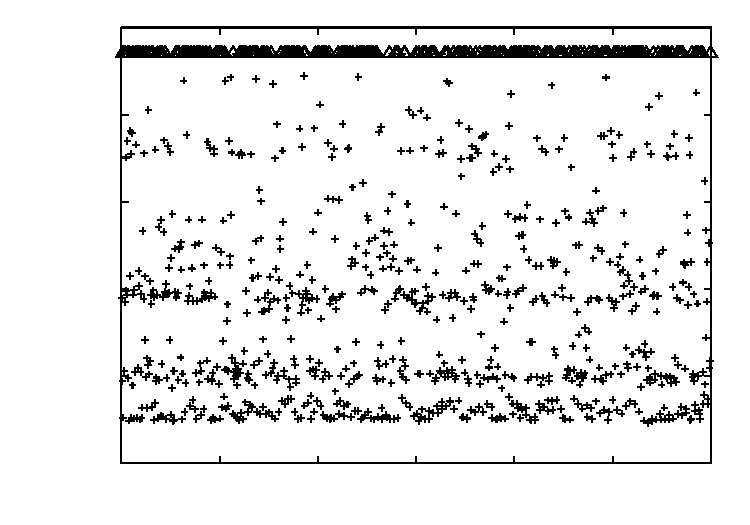
\includegraphics{fig2/ker23TotSched}}%
    \gplfronttext
  \end{picture}%
\endgroup
}}}

  \subfloat[\textbf{Linux$^{\mathbf{Prt}}$ - Sem carga} \newline
  \vskip 1mm {\footnotesize VM: 2.1, DP: 0.2, Min: 1.2, Max: 9.4}]{%
    \label{fig:preSemSched}%
    {\scalebox{\scaleFact}{% GNUPLOT: LaTeX picture with Postscript
\begingroup
  \makeatletter
  \providecommand\color[2][]{%
    \GenericError{(gnuplot) \space\space\space\@spaces}{%
      Package color not loaded in conjunction with
      terminal option `colourtext'%
    }{See the gnuplot documentation for explanation.%
    }{Either use 'blacktext' in gnuplot or load the package
      color.sty in LaTeX.}%
    \renewcommand\color[2][]{}%
  }%
  \providecommand\includegraphics[2][]{%
    \GenericError{(gnuplot) \space\space\space\@spaces}{%
      Package graphicx or graphics not loaded%
    }{See the gnuplot documentation for explanation.%
    }{The gnuplot epslatex terminal needs graphicx.sty or graphics.sty.}%
    \renewcommand\includegraphics[2][]{}%
  }%
  \providecommand\rotatebox[2]{#2}%
  \@ifundefined{ifGPcolor}{%
    \newif\ifGPcolor
    \GPcolorfalse
  }{}%
  \@ifundefined{ifGPblacktext}{%
    \newif\ifGPblacktext
    \GPblacktextfalse
  }{}%
  % define a \g@addto@macro without @ in the name:
  \let\gplgaddtomacro\g@addto@macro
  % define empty templates for all commands taking text:
  \gdef\gplbacktext{}%
  \gdef\gplfronttext{}%
  \makeatother
  \ifGPblacktext
    % no textcolor at all
    \def\colorrgb#1{}%
    \def\colorgray#1{}%
  \else
    % gray or color?
    \ifGPcolor
      \def\colorrgb#1{\color[rgb]{#1}}%
      \def\colorgray#1{\color[gray]{#1}}%
      \expandafter\def\csname LTw\endcsname{\color{white}}%
      \expandafter\def\csname LTb\endcsname{\color{black}}%
      \expandafter\def\csname LTa\endcsname{\color{black}}%
      \expandafter\def\csname LT0\endcsname{\color[rgb]{1,0,0}}%
      \expandafter\def\csname LT1\endcsname{\color[rgb]{0,1,0}}%
      \expandafter\def\csname LT2\endcsname{\color[rgb]{0,0,1}}%
      \expandafter\def\csname LT3\endcsname{\color[rgb]{1,0,1}}%
      \expandafter\def\csname LT4\endcsname{\color[rgb]{0,1,1}}%
      \expandafter\def\csname LT5\endcsname{\color[rgb]{1,1,0}}%
      \expandafter\def\csname LT6\endcsname{\color[rgb]{0,0,0}}%
      \expandafter\def\csname LT7\endcsname{\color[rgb]{1,0.3,0}}%
      \expandafter\def\csname LT8\endcsname{\color[rgb]{0.5,0.5,0.5}}%
    \else
      % gray
      \def\colorrgb#1{\color{black}}%
      \def\colorgray#1{\color[gray]{#1}}%
      \expandafter\def\csname LTw\endcsname{\color{white}}%
      \expandafter\def\csname LTb\endcsname{\color{black}}%
      \expandafter\def\csname LTa\endcsname{\color{black}}%
      \expandafter\def\csname LT0\endcsname{\color{black}}%
      \expandafter\def\csname LT1\endcsname{\color{black}}%
      \expandafter\def\csname LT2\endcsname{\color{black}}%
      \expandafter\def\csname LT3\endcsname{\color{black}}%
      \expandafter\def\csname LT4\endcsname{\color{black}}%
      \expandafter\def\csname LT5\endcsname{\color{black}}%
      \expandafter\def\csname LT6\endcsname{\color{black}}%
      \expandafter\def\csname LT7\endcsname{\color{black}}%
      \expandafter\def\csname LT8\endcsname{\color{black}}%
    \fi
  \fi
  \setlength{\unitlength}{0.0500bp}%
  \begin{picture}(7200.00,5040.00)%
    \gplgaddtomacro\gplbacktext{%
      \csname LTb\endcsname%
      \put(1034,594){\makebox(0,0)[r]{\strut{}$0.0$}}%
      \put(1034,1640){\makebox(0,0)[r]{\strut{}$5.0$}}%
      \put(1034,2685){\makebox(0,0)[r]{\strut{}$10.0$}}%
      \put(1034,3731){\makebox(0,0)[r]{\strut{}$15.0$}}%
      \put(1034,4776){\makebox(0,0)[r]{\strut{}$20.0$}}%
      \put(1166,374){\makebox(0,0){\strut{}$ 0$}}%
      \put(2109,374){\makebox(0,0){\strut{}$ 10$}}%
      \put(3053,374){\makebox(0,0){\strut{}$ 20$}}%
      \put(3996,374){\makebox(0,0){\strut{}$ 30$}}%
      \put(4939,374){\makebox(0,0){\strut{}$ 40$}}%
      \put(5883,374){\makebox(0,0){\strut{}$ 50$}}%
      \put(6826,374){\makebox(0,0){\strut{}$ 60$}}%
      \put(396,2685){\rotatebox{90}{\makebox(0,0){\strut{}Lat\^encia em $\mu s$}}}%
      \put(3996,110){\makebox(0,0){\strut{}Tempo de observa\c{c}\~ao em $s$}}%
    }%
    \gplgaddtomacro\gplfronttext{%
    }%
    \gplbacktext
    \put(0,0){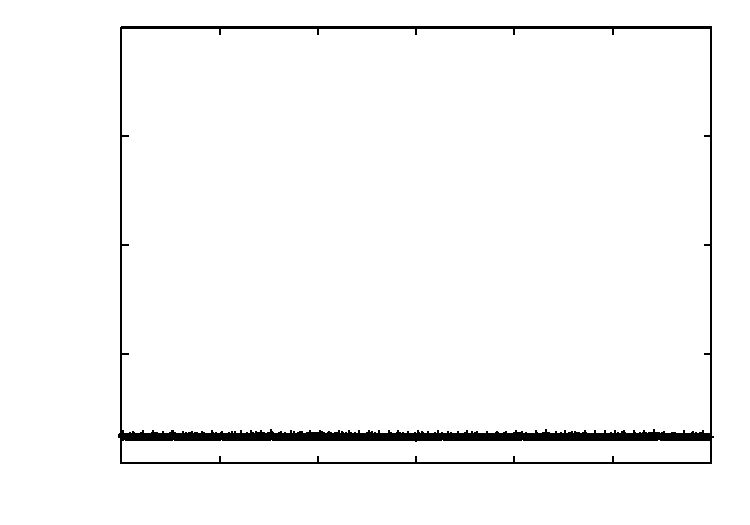
\includegraphics{fig/preSemSched.pdf}}%
    \gplfronttext
  \end{picture}%
\endgroup
}}}
  \hspace{\spaceFact}%
  \subfloat[\textbf{Linux$^{\mathbf{Prt}}$ - Com carga} \newline
  \vskip 1mm {\footnotesize VM: 3.8, DP: 2.8, Min: 1.1, Max: 27.4}]{%
    \label{fig:preTotSched}%
    {\scalebox{\scaleFact}{% GNUPLOT: LaTeX picture with Postscript
\begingroup
  \makeatletter
  \providecommand\color[2][]{%
    \GenericError{(gnuplot) \space\space\space\@spaces}{%
      Package color not loaded in conjunction with
      terminal option `colourtext'%
    }{See the gnuplot documentation for explanation.%
    }{Either use 'blacktext' in gnuplot or load the package
      color.sty in LaTeX.}%
    \renewcommand\color[2][]{}%
  }%
  \providecommand\includegraphics[2][]{%
    \GenericError{(gnuplot) \space\space\space\@spaces}{%
      Package graphicx or graphics not loaded%
    }{See the gnuplot documentation for explanation.%
    }{The gnuplot epslatex terminal needs graphicx.sty or graphics.sty.}%
    \renewcommand\includegraphics[2][]{}%
  }%
  \providecommand\rotatebox[2]{#2}%
  \@ifundefined{ifGPcolor}{%
    \newif\ifGPcolor
    \GPcolorfalse
  }{}%
  \@ifundefined{ifGPblacktext}{%
    \newif\ifGPblacktext
    \GPblacktextfalse
  }{}%
  % define a \g@addto@macro without @ in the name:
  \let\gplgaddtomacro\g@addto@macro
  % define empty templates for all commands taking text:
  \gdef\gplbacktext{}%
  \gdef\gplfronttext{}%
  \makeatother
  \ifGPblacktext
    % no textcolor at all
    \def\colorrgb#1{}%
    \def\colorgray#1{}%
  \else
    % gray or color?
    \ifGPcolor
      \def\colorrgb#1{\color[rgb]{#1}}%
      \def\colorgray#1{\color[gray]{#1}}%
      \expandafter\def\csname LTw\endcsname{\color{white}}%
      \expandafter\def\csname LTb\endcsname{\color{black}}%
      \expandafter\def\csname LTa\endcsname{\color{black}}%
      \expandafter\def\csname LT0\endcsname{\color[rgb]{1,0,0}}%
      \expandafter\def\csname LT1\endcsname{\color[rgb]{0,1,0}}%
      \expandafter\def\csname LT2\endcsname{\color[rgb]{0,0,1}}%
      \expandafter\def\csname LT3\endcsname{\color[rgb]{1,0,1}}%
      \expandafter\def\csname LT4\endcsname{\color[rgb]{0,1,1}}%
      \expandafter\def\csname LT5\endcsname{\color[rgb]{1,1,0}}%
      \expandafter\def\csname LT6\endcsname{\color[rgb]{0,0,0}}%
      \expandafter\def\csname LT7\endcsname{\color[rgb]{1,0.3,0}}%
      \expandafter\def\csname LT8\endcsname{\color[rgb]{0.5,0.5,0.5}}%
    \else
      % gray
      \def\colorrgb#1{\color{black}}%
      \def\colorgray#1{\color[gray]{#1}}%
      \expandafter\def\csname LTw\endcsname{\color{white}}%
      \expandafter\def\csname LTb\endcsname{\color{black}}%
      \expandafter\def\csname LTa\endcsname{\color{black}}%
      \expandafter\def\csname LT0\endcsname{\color{black}}%
      \expandafter\def\csname LT1\endcsname{\color{black}}%
      \expandafter\def\csname LT2\endcsname{\color{black}}%
      \expandafter\def\csname LT3\endcsname{\color{black}}%
      \expandafter\def\csname LT4\endcsname{\color{black}}%
      \expandafter\def\csname LT5\endcsname{\color{black}}%
      \expandafter\def\csname LT6\endcsname{\color{black}}%
      \expandafter\def\csname LT7\endcsname{\color{black}}%
      \expandafter\def\csname LT8\endcsname{\color{black}}%
    \fi
  \fi
  \setlength{\unitlength}{0.0500bp}%
  \begin{picture}(7200.00,5040.00)%
    \gplgaddtomacro\gplbacktext{%
      \csname LTb\endcsname%
      \put(1034,594){\makebox(0,0)[r]{\strut{}$0.0$}}%
      \put(1034,1640){\makebox(0,0)[r]{\strut{}$5.0$}}%
      \put(1034,2685){\makebox(0,0)[r]{\strut{}$10.0$}}%
      \put(1034,3731){\makebox(0,0)[r]{\strut{}$15.0$}}%
      \put(1034,4776){\makebox(0,0)[r]{\strut{}$20.0$}}%
      \put(1166,374){\makebox(0,0){\strut{}$ 0$}}%
      \put(2109,374){\makebox(0,0){\strut{}$ 10$}}%
      \put(3053,374){\makebox(0,0){\strut{}$ 20$}}%
      \put(3996,374){\makebox(0,0){\strut{}$ 30$}}%
      \put(4939,374){\makebox(0,0){\strut{}$ 40$}}%
      \put(5883,374){\makebox(0,0){\strut{}$ 50$}}%
      \put(6826,374){\makebox(0,0){\strut{}$ 60$}}%
      \put(396,2685){\rotatebox{90}{\makebox(0,0){\strut{}Lat\^encia em $\mu s$}}}%
      \put(3996,110){\makebox(0,0){\strut{}Tempo de observa\c{c}\~ao em $s$}}%
    }%
    \gplgaddtomacro\gplfronttext{%
    }%
    \gplbacktext
    \put(0,0){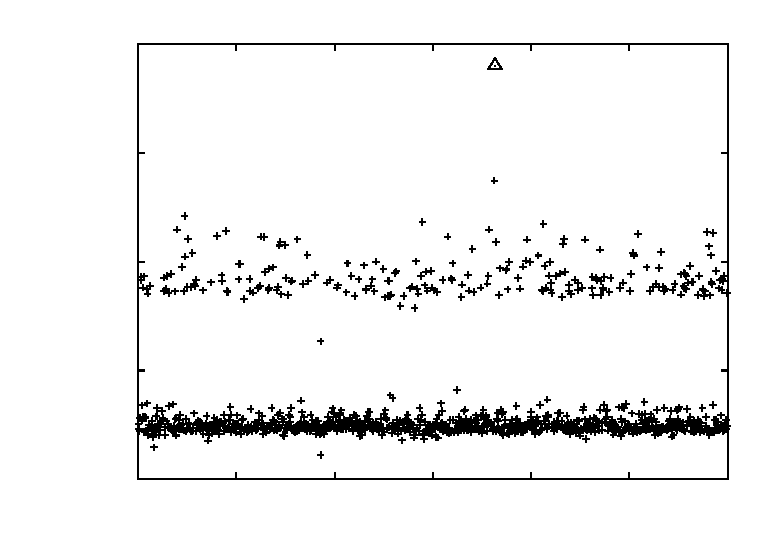
\includegraphics{fig/preTotSched}}%
    \gplfronttext
  \end{picture}%
\endgroup
}}}

  \subfloat[\textbf{Linux$^{\mathbf{Rtai}}$ - Sem carga} \newline
  \vskip 1mm {\footnotesize VM: 0.6, DP: 0.3, Min: 0.4, Max: 3.8}]{%
    \label{fig:rtaiSemSched}%
    {\scalebox{\scaleFact}{% GNUPLOT: LaTeX picture with Postscript
\begingroup
  \makeatletter
  \providecommand\color[2][]{%
    \GenericError{(gnuplot) \space\space\space\@spaces}{%
      Package color not loaded in conjunction with
      terminal option `colourtext'%
    }{See the gnuplot documentation for explanation.%
    }{Either use 'blacktext' in gnuplot or load the package
      color.sty in LaTeX.}%
    \renewcommand\color[2][]{}%
  }%
  \providecommand\includegraphics[2][]{%
    \GenericError{(gnuplot) \space\space\space\@spaces}{%
      Package graphicx or graphics not loaded%
    }{See the gnuplot documentation for explanation.%
    }{The gnuplot epslatex terminal needs graphicx.sty or graphics.sty.}%
    \renewcommand\includegraphics[2][]{}%
  }%
  \providecommand\rotatebox[2]{#2}%
  \@ifundefined{ifGPcolor}{%
    \newif\ifGPcolor
    \GPcolorfalse
  }{}%
  \@ifundefined{ifGPblacktext}{%
    \newif\ifGPblacktext
    \GPblacktextfalse
  }{}%
  % define a \g@addto@macro without @ in the name:
  \let\gplgaddtomacro\g@addto@macro
  % define empty templates for all commands taking text:
  \gdef\gplbacktext{}%
  \gdef\gplfronttext{}%
  \makeatother
  \ifGPblacktext
    % no textcolor at all
    \def\colorrgb#1{}%
    \def\colorgray#1{}%
  \else
    % gray or color?
    \ifGPcolor
      \def\colorrgb#1{\color[rgb]{#1}}%
      \def\colorgray#1{\color[gray]{#1}}%
      \expandafter\def\csname LTw\endcsname{\color{white}}%
      \expandafter\def\csname LTb\endcsname{\color{black}}%
      \expandafter\def\csname LTa\endcsname{\color{black}}%
      \expandafter\def\csname LT0\endcsname{\color[rgb]{1,0,0}}%
      \expandafter\def\csname LT1\endcsname{\color[rgb]{0,1,0}}%
      \expandafter\def\csname LT2\endcsname{\color[rgb]{0,0,1}}%
      \expandafter\def\csname LT3\endcsname{\color[rgb]{1,0,1}}%
      \expandafter\def\csname LT4\endcsname{\color[rgb]{0,1,1}}%
      \expandafter\def\csname LT5\endcsname{\color[rgb]{1,1,0}}%
      \expandafter\def\csname LT6\endcsname{\color[rgb]{0,0,0}}%
      \expandafter\def\csname LT7\endcsname{\color[rgb]{1,0.3,0}}%
      \expandafter\def\csname LT8\endcsname{\color[rgb]{0.5,0.5,0.5}}%
    \else
      % gray
      \def\colorrgb#1{\color{black}}%
      \def\colorgray#1{\color[gray]{#1}}%
      \expandafter\def\csname LTw\endcsname{\color{white}}%
      \expandafter\def\csname LTb\endcsname{\color{black}}%
      \expandafter\def\csname LTa\endcsname{\color{black}}%
      \expandafter\def\csname LT0\endcsname{\color{black}}%
      \expandafter\def\csname LT1\endcsname{\color{black}}%
      \expandafter\def\csname LT2\endcsname{\color{black}}%
      \expandafter\def\csname LT3\endcsname{\color{black}}%
      \expandafter\def\csname LT4\endcsname{\color{black}}%
      \expandafter\def\csname LT5\endcsname{\color{black}}%
      \expandafter\def\csname LT6\endcsname{\color{black}}%
      \expandafter\def\csname LT7\endcsname{\color{black}}%
      \expandafter\def\csname LT8\endcsname{\color{black}}%
    \fi
  \fi
  \setlength{\unitlength}{0.0500bp}%
  \begin{picture}(7200.00,5040.00)%
    \gplgaddtomacro\gplbacktext{%
      \csname LTb\endcsname%
      \put(1034,594){\makebox(0,0)[r]{\strut{}$0.0$}}%
      \put(1034,1640){\makebox(0,0)[r]{\strut{}$5.0$}}%
      \put(1034,2685){\makebox(0,0)[r]{\strut{}$10.0$}}%
      \put(1034,3731){\makebox(0,0)[r]{\strut{}$15.0$}}%
      \put(1034,4776){\makebox(0,0)[r]{\strut{}$20.0$}}%
      \put(1166,374){\makebox(0,0){\strut{}$ 0$}}%
      \put(2109,374){\makebox(0,0){\strut{}$ 10$}}%
      \put(3053,374){\makebox(0,0){\strut{}$ 20$}}%
      \put(3996,374){\makebox(0,0){\strut{}$ 30$}}%
      \put(4939,374){\makebox(0,0){\strut{}$ 40$}}%
      \put(5883,374){\makebox(0,0){\strut{}$ 50$}}%
      \put(6826,374){\makebox(0,0){\strut{}$ 60$}}%
      \put(396,2685){\rotatebox{90}{\makebox(0,0){\strut{}Latency ($\mu s$)}}}%
      \put(3996,110){\makebox(0,0){\strut{}Time ($s$)}}%
    }%
    \gplgaddtomacro\gplfronttext{%
    }%
    \gplbacktext
    \put(0,0){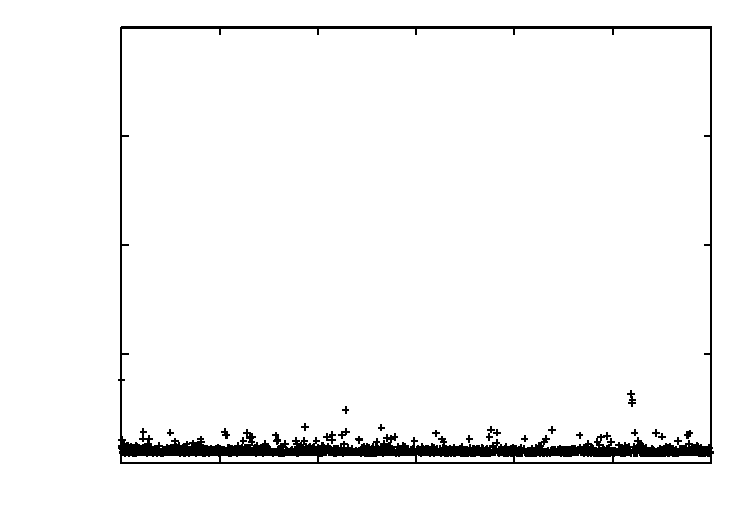
\includegraphics{fig/rtaiSemSched.pdf}}%
    \gplfronttext
  \end{picture}%
\endgroup
}}} \hspace{4pt}%
  \hspace{\spaceFact}%
  \subfloat[\textbf{Linux$^{\mathbf{Rtai}}$ - Com carga} \newline
  \vskip 1mm  {\footnotesize VM: 4.4, DP: 0.7,  Min: 0.5, Max: 14.7}]{%
    \label{fig:rtaiTotSched}%
    {\scalebox{\scaleFact}{% GNUPLOT: LaTeX picture with Postscript
\begingroup
  \makeatletter
  \providecommand\color[2][]{%
    \GenericError{(gnuplot) \space\space\space\@spaces}{%
      Package color not loaded in conjunction with
      terminal option `colourtext'%
    }{See the gnuplot documentation for explanation.%
    }{Either use 'blacktext' in gnuplot or load the package
      color.sty in LaTeX.}%
    \renewcommand\color[2][]{}%
  }%
  \providecommand\includegraphics[2][]{%
    \GenericError{(gnuplot) \space\space\space\@spaces}{%
      Package graphicx or graphics not loaded%
    }{See the gnuplot documentation for explanation.%
    }{The gnuplot epslatex terminal needs graphicx.sty or graphics.sty.}%
    \renewcommand\includegraphics[2][]{}%
  }%
  \providecommand\rotatebox[2]{#2}%
  \@ifundefined{ifGPcolor}{%
    \newif\ifGPcolor
    \GPcolorfalse
  }{}%
  \@ifundefined{ifGPblacktext}{%
    \newif\ifGPblacktext
    \GPblacktextfalse
  }{}%
  % define a \g@addto@macro without @ in the name:
  \let\gplgaddtomacro\g@addto@macro
  % define empty templates for all commands taking text:
  \gdef\gplbacktext{}%
  \gdef\gplfronttext{}%
  \makeatother
  \ifGPblacktext
    % no textcolor at all
    \def\colorrgb#1{}%
    \def\colorgray#1{}%
  \else
    % gray or color?
    \ifGPcolor
      \def\colorrgb#1{\color[rgb]{#1}}%
      \def\colorgray#1{\color[gray]{#1}}%
      \expandafter\def\csname LTw\endcsname{\color{white}}%
      \expandafter\def\csname LTb\endcsname{\color{black}}%
      \expandafter\def\csname LTa\endcsname{\color{black}}%
      \expandafter\def\csname LT0\endcsname{\color[rgb]{1,0,0}}%
      \expandafter\def\csname LT1\endcsname{\color[rgb]{0,1,0}}%
      \expandafter\def\csname LT2\endcsname{\color[rgb]{0,0,1}}%
      \expandafter\def\csname LT3\endcsname{\color[rgb]{1,0,1}}%
      \expandafter\def\csname LT4\endcsname{\color[rgb]{0,1,1}}%
      \expandafter\def\csname LT5\endcsname{\color[rgb]{1,1,0}}%
      \expandafter\def\csname LT6\endcsname{\color[rgb]{0,0,0}}%
      \expandafter\def\csname LT7\endcsname{\color[rgb]{1,0.3,0}}%
      \expandafter\def\csname LT8\endcsname{\color[rgb]{0.5,0.5,0.5}}%
    \else
      % gray
      \def\colorrgb#1{\color{black}}%
      \def\colorgray#1{\color[gray]{#1}}%
      \expandafter\def\csname LTw\endcsname{\color{white}}%
      \expandafter\def\csname LTb\endcsname{\color{black}}%
      \expandafter\def\csname LTa\endcsname{\color{black}}%
      \expandafter\def\csname LT0\endcsname{\color{black}}%
      \expandafter\def\csname LT1\endcsname{\color{black}}%
      \expandafter\def\csname LT2\endcsname{\color{black}}%
      \expandafter\def\csname LT3\endcsname{\color{black}}%
      \expandafter\def\csname LT4\endcsname{\color{black}}%
      \expandafter\def\csname LT5\endcsname{\color{black}}%
      \expandafter\def\csname LT6\endcsname{\color{black}}%
      \expandafter\def\csname LT7\endcsname{\color{black}}%
      \expandafter\def\csname LT8\endcsname{\color{black}}%
    \fi
  \fi
  \setlength{\unitlength}{0.0500bp}%
  \begin{picture}(7200.00,5040.00)%
    \gplgaddtomacro\gplbacktext{%
      \csname LTb\endcsname%
      \put(1034,594){\makebox(0,0)[r]{\strut{}$0.0$}}%
      \put(1034,1640){\makebox(0,0)[r]{\strut{}$5.0$}}%
      \put(1034,2685){\makebox(0,0)[r]{\strut{}$10.0$}}%
      \put(1034,3731){\makebox(0,0)[r]{\strut{}$15.0$}}%
      \put(1034,4776){\makebox(0,0)[r]{\strut{}$20.0$}}%
      \put(1166,374){\makebox(0,0){\strut{}$ 0$}}%
      \put(2109,374){\makebox(0,0){\strut{}$ 10$}}%
      \put(3053,374){\makebox(0,0){\strut{}$ 20$}}%
      \put(3996,374){\makebox(0,0){\strut{}$ 30$}}%
      \put(4939,374){\makebox(0,0){\strut{}$ 40$}}%
      \put(5883,374){\makebox(0,0){\strut{}$ 50$}}%
      \put(6826,374){\makebox(0,0){\strut{}$ 60$}}%
      \put(396,2685){\rotatebox{90}{\makebox(0,0){\strut{}Lat\^encia em $\mu s$}}}%
      \put(3996,110){\makebox(0,0){\strut{}Tempo de observa\c{c}\~ao em $s$}}%
    }%
    \gplgaddtomacro\gplfronttext{%
    }%
    \gplbacktext
    \put(0,0){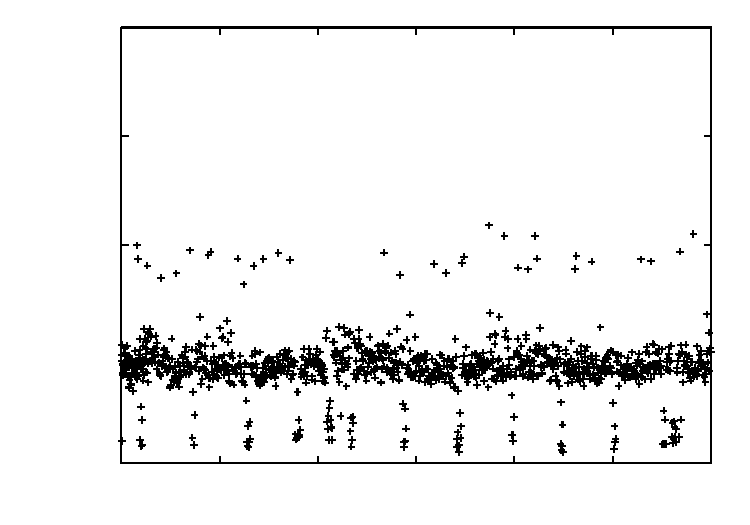
\includegraphics{fig/rtaiTotSched.pdf}}%
    \gplfronttext
  \end{picture}%
\endgroup
}}} \hspace{4pt}%

  \subfloat[\textbf{Linux$^{\mathbf{Xen}}$ - Sem carga} \newline
  \vskip 1mm {\footnotesize VM: 2.1, DP: 0.5, Min: 1.8, Max: 8.4}]{%
    \label{fig:xenSemSched}%
    {\scalebox{\scaleFact}{% GNUPLOT: LaTeX picture with Postscript
\begingroup
  \makeatletter
  \providecommand\color[2][]{%
    \GenericError{(gnuplot) \space\space\space\@spaces}{%
      Package color not loaded in conjunction with
      terminal option `colourtext'%
    }{See the gnuplot documentation for explanation.%
    }{Either use 'blacktext' in gnuplot or load the package
      color.sty in LaTeX.}%
    \renewcommand\color[2][]{}%
  }%
  \providecommand\includegraphics[2][]{%
    \GenericError{(gnuplot) \space\space\space\@spaces}{%
      Package graphicx or graphics not loaded%
    }{See the gnuplot documentation for explanation.%
    }{The gnuplot epslatex terminal needs graphicx.sty or graphics.sty.}%
    \renewcommand\includegraphics[2][]{}%
  }%
  \providecommand\rotatebox[2]{#2}%
  \@ifundefined{ifGPcolor}{%
    \newif\ifGPcolor
    \GPcolorfalse
  }{}%
  \@ifundefined{ifGPblacktext}{%
    \newif\ifGPblacktext
    \GPblacktextfalse
  }{}%
  % define a \g@addto@macro without @ in the name:
  \let\gplgaddtomacro\g@addto@macro
  % define empty templates for all commands taking text:
  \gdef\gplbacktext{}%
  \gdef\gplfronttext{}%
  \makeatother
  \ifGPblacktext
    % no textcolor at all
    \def\colorrgb#1{}%
    \def\colorgray#1{}%
  \else
    % gray or color?
    \ifGPcolor
      \def\colorrgb#1{\color[rgb]{#1}}%
      \def\colorgray#1{\color[gray]{#1}}%
      \expandafter\def\csname LTw\endcsname{\color{white}}%
      \expandafter\def\csname LTb\endcsname{\color{black}}%
      \expandafter\def\csname LTa\endcsname{\color{black}}%
      \expandafter\def\csname LT0\endcsname{\color[rgb]{1,0,0}}%
      \expandafter\def\csname LT1\endcsname{\color[rgb]{0,1,0}}%
      \expandafter\def\csname LT2\endcsname{\color[rgb]{0,0,1}}%
      \expandafter\def\csname LT3\endcsname{\color[rgb]{1,0,1}}%
      \expandafter\def\csname LT4\endcsname{\color[rgb]{0,1,1}}%
      \expandafter\def\csname LT5\endcsname{\color[rgb]{1,1,0}}%
      \expandafter\def\csname LT6\endcsname{\color[rgb]{0,0,0}}%
      \expandafter\def\csname LT7\endcsname{\color[rgb]{1,0.3,0}}%
      \expandafter\def\csname LT8\endcsname{\color[rgb]{0.5,0.5,0.5}}%
    \else
      % gray
      \def\colorrgb#1{\color{black}}%
      \def\colorgray#1{\color[gray]{#1}}%
      \expandafter\def\csname LTw\endcsname{\color{white}}%
      \expandafter\def\csname LTb\endcsname{\color{black}}%
      \expandafter\def\csname LTa\endcsname{\color{black}}%
      \expandafter\def\csname LT0\endcsname{\color{black}}%
      \expandafter\def\csname LT1\endcsname{\color{black}}%
      \expandafter\def\csname LT2\endcsname{\color{black}}%
      \expandafter\def\csname LT3\endcsname{\color{black}}%
      \expandafter\def\csname LT4\endcsname{\color{black}}%
      \expandafter\def\csname LT5\endcsname{\color{black}}%
      \expandafter\def\csname LT6\endcsname{\color{black}}%
      \expandafter\def\csname LT7\endcsname{\color{black}}%
      \expandafter\def\csname LT8\endcsname{\color{black}}%
    \fi
  \fi
  \setlength{\unitlength}{0.0500bp}%
  \begin{picture}(7200.00,5040.00)%
    \gplgaddtomacro\gplbacktext{%
      \csname LTb\endcsname%
      \put(1034,594){\makebox(0,0)[r]{\strut{}$0.0$}}%
      \put(1034,1640){\makebox(0,0)[r]{\strut{}$5.0$}}%
      \put(1034,2685){\makebox(0,0)[r]{\strut{}$10.0$}}%
      \put(1034,3731){\makebox(0,0)[r]{\strut{}$15.0$}}%
      \put(1034,4776){\makebox(0,0)[r]{\strut{}$20.0$}}%
      \put(1166,374){\makebox(0,0){\strut{}$ 0$}}%
      \put(2109,374){\makebox(0,0){\strut{}$ 10$}}%
      \put(3053,374){\makebox(0,0){\strut{}$ 20$}}%
      \put(3996,374){\makebox(0,0){\strut{}$ 30$}}%
      \put(4939,374){\makebox(0,0){\strut{}$ 40$}}%
      \put(5883,374){\makebox(0,0){\strut{}$ 50$}}%
      \put(6826,374){\makebox(0,0){\strut{}$ 60$}}%
      \put(396,2685){\rotatebox{90}{\makebox(0,0){\strut{}Lat\^encia em $\mu s$}}}%
      \put(3996,110){\makebox(0,0){\strut{}Tempo de observa\c{c}\~ao em $s$}}%
    }%
    \gplgaddtomacro\gplfronttext{%
    }%
    \gplbacktext
    \put(0,0){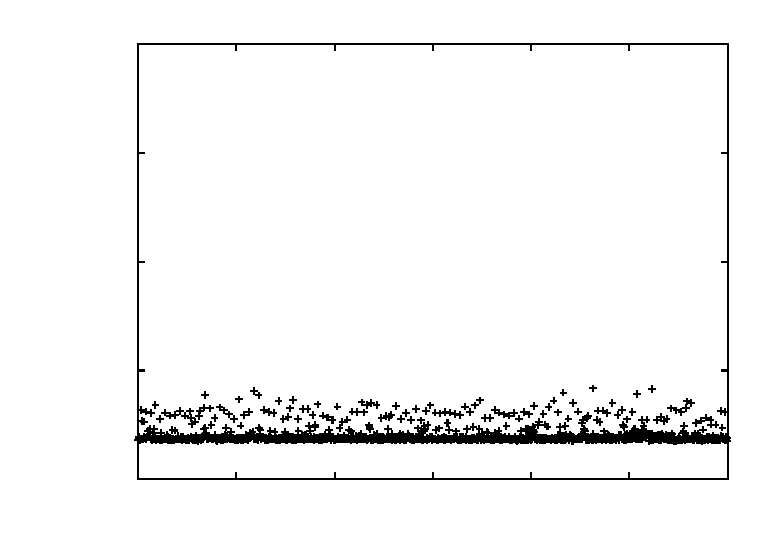
\includegraphics{fig/xenSemSched}}%
    \gplfronttext
  \end{picture}%
\endgroup
}}}
  \hspace{\spaceFact}%
  \subfloat[\textbf{Linux$^{\mathbf{Xen}}$ - Com carga} \newline
  \vskip 1mm {\footnotesize VM: 8.7, DP: 0.3, Min: 1.8, Max: 18.7}]{%
    \label{fig:xenTotSched}%
    {\scalebox{\scaleFact}{% GNUPLOT: LaTeX picture with Postscript
\begingroup
  \makeatletter
  \providecommand\color[2][]{%
    \GenericError{(gnuplot) \space\space\space\@spaces}{%
      Package color not loaded in conjunction with
      terminal option `colourtext'%
    }{See the gnuplot documentation for explanation.%
    }{Either use 'blacktext' in gnuplot or load the package
      color.sty in LaTeX.}%
    \renewcommand\color[2][]{}%
  }%
  \providecommand\includegraphics[2][]{%
    \GenericError{(gnuplot) \space\space\space\@spaces}{%
      Package graphicx or graphics not loaded%
    }{See the gnuplot documentation for explanation.%
    }{The gnuplot epslatex terminal needs graphicx.sty or graphics.sty.}%
    \renewcommand\includegraphics[2][]{}%
  }%
  \providecommand\rotatebox[2]{#2}%
  \@ifundefined{ifGPcolor}{%
    \newif\ifGPcolor
    \GPcolorfalse
  }{}%
  \@ifundefined{ifGPblacktext}{%
    \newif\ifGPblacktext
    \GPblacktextfalse
  }{}%
  % define a \g@addto@macro without @ in the name:
  \let\gplgaddtomacro\g@addto@macro
  % define empty templates for all commands taking text:
  \gdef\gplbacktext{}%
  \gdef\gplfronttext{}%
  \makeatother
  \ifGPblacktext
    % no textcolor at all
    \def\colorrgb#1{}%
    \def\colorgray#1{}%
  \else
    % gray or color?
    \ifGPcolor
      \def\colorrgb#1{\color[rgb]{#1}}%
      \def\colorgray#1{\color[gray]{#1}}%
      \expandafter\def\csname LTw\endcsname{\color{white}}%
      \expandafter\def\csname LTb\endcsname{\color{black}}%
      \expandafter\def\csname LTa\endcsname{\color{black}}%
      \expandafter\def\csname LT0\endcsname{\color[rgb]{1,0,0}}%
      \expandafter\def\csname LT1\endcsname{\color[rgb]{0,1,0}}%
      \expandafter\def\csname LT2\endcsname{\color[rgb]{0,0,1}}%
      \expandafter\def\csname LT3\endcsname{\color[rgb]{1,0,1}}%
      \expandafter\def\csname LT4\endcsname{\color[rgb]{0,1,1}}%
      \expandafter\def\csname LT5\endcsname{\color[rgb]{1,1,0}}%
      \expandafter\def\csname LT6\endcsname{\color[rgb]{0,0,0}}%
      \expandafter\def\csname LT7\endcsname{\color[rgb]{1,0.3,0}}%
      \expandafter\def\csname LT8\endcsname{\color[rgb]{0.5,0.5,0.5}}%
    \else
      % gray
      \def\colorrgb#1{\color{black}}%
      \def\colorgray#1{\color[gray]{#1}}%
      \expandafter\def\csname LTw\endcsname{\color{white}}%
      \expandafter\def\csname LTb\endcsname{\color{black}}%
      \expandafter\def\csname LTa\endcsname{\color{black}}%
      \expandafter\def\csname LT0\endcsname{\color{black}}%
      \expandafter\def\csname LT1\endcsname{\color{black}}%
      \expandafter\def\csname LT2\endcsname{\color{black}}%
      \expandafter\def\csname LT3\endcsname{\color{black}}%
      \expandafter\def\csname LT4\endcsname{\color{black}}%
      \expandafter\def\csname LT5\endcsname{\color{black}}%
      \expandafter\def\csname LT6\endcsname{\color{black}}%
      \expandafter\def\csname LT7\endcsname{\color{black}}%
      \expandafter\def\csname LT8\endcsname{\color{black}}%
    \fi
  \fi
  \setlength{\unitlength}{0.0500bp}%
  \begin{picture}(7200.00,5040.00)%
    \gplgaddtomacro\gplbacktext{%
      \csname LTb\endcsname%
      \put(1034,594){\makebox(0,0)[r]{\strut{}$0.0$}}%
      \put(1034,1291){\makebox(0,0)[r]{\strut{}$5.0$}}%
      \put(1034,1988){\makebox(0,0)[r]{\strut{}$10.0$}}%
      \put(1034,2685){\makebox(0,0)[r]{\strut{}$15.0$}}%
      \put(1034,3382){\makebox(0,0)[r]{\strut{}$20.0$}}%
      \put(1034,4079){\makebox(0,0)[r]{\strut{}$25.0$}}%
      \put(1034,4776){\makebox(0,0)[r]{\strut{}$30.0$}}%
      \put(1166,374){\makebox(0,0){\strut{}$ 0$}}%
      \put(2109,374){\makebox(0,0){\strut{}$ 10$}}%
      \put(3053,374){\makebox(0,0){\strut{}$ 20$}}%
      \put(3996,374){\makebox(0,0){\strut{}$ 30$}}%
      \put(4939,374){\makebox(0,0){\strut{}$ 40$}}%
      \put(5883,374){\makebox(0,0){\strut{}$ 50$}}%
      \put(6826,374){\makebox(0,0){\strut{}$ 60$}}%
      \put(396,2685){\rotatebox{90}{\makebox(0,0){\strut{}Lat\^encia em $\mu s$}}}%
      \put(3996,110){\makebox(0,0){\strut{}Tempo de observa\c{c}\~ao em $s$}}%
    }%
    \gplgaddtomacro\gplfronttext{%
    }%
    \gplbacktext
    \put(0,0){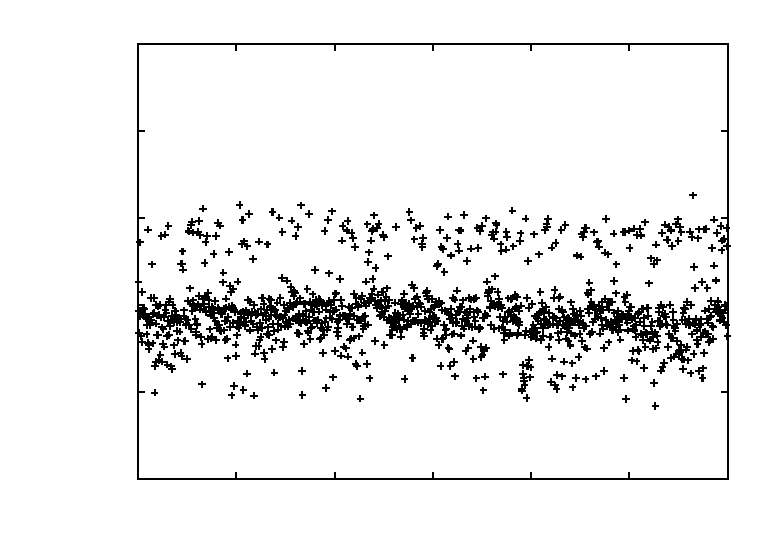
\includegraphics{fig2/xenTotSched}}%
    \gplfronttext
  \end{picture}%
\endgroup
}}}

  \caption[]{Lat�ncia de ativa��o com freq��ncia de escrita
    na PP de $20 Hz$.}
  \label{fig:latAtiv}%
\end{figure}

� interessante ainda observar o comportamento de
Linux$^{\mathbf{Prt}}$ sem utilizar o contexto de \ing{threads} de
interrup��o, isto �, com a op��o \cod{IRQF\_NODELAY}, comentada
anteriormente. Como pode ser observado na figura \ref{fig:latAtivND},
apesar de as lat�ncias de ativa��o sem estresse apresentar uns bons
resultados em compara��o ao Linux$^{\mathbf{Prt}}$, seus valores com
estresse indicam um comportamento menos previs�vel que o
Linux$^{\mathbf{Xen}}$.

\begin{figure}%
  \centering
  \subfloat[\textbf{Linux$^{\mathbf{Prt}}$ - Sem carga} \newline
  \vskip 1mm VM:     5.3, DP:     0.3,  Min:     5.0, Max:    13.1]{%
    \label{fig:preSemSchedND}%
    {\scalebox{0.58}{% GNUPLOT: LaTeX picture with Postscript
\begingroup
  \makeatletter
  \providecommand\color[2][]{%
    \GenericError{(gnuplot) \space\space\space\@spaces}{%
      Package color not loaded in conjunction with
      terminal option `colourtext'%
    }{See the gnuplot documentation for explanation.%
    }{Either use 'blacktext' in gnuplot or load the package
      color.sty in LaTeX.}%
    \renewcommand\color[2][]{}%
  }%
  \providecommand\includegraphics[2][]{%
    \GenericError{(gnuplot) \space\space\space\@spaces}{%
      Package graphicx or graphics not loaded%
    }{See the gnuplot documentation for explanation.%
    }{The gnuplot epslatex terminal needs graphicx.sty or graphics.sty.}%
    \renewcommand\includegraphics[2][]{}%
  }%
  \providecommand\rotatebox[2]{#2}%
  \@ifundefined{ifGPcolor}{%
    \newif\ifGPcolor
    \GPcolorfalse
  }{}%
  \@ifundefined{ifGPblacktext}{%
    \newif\ifGPblacktext
    \GPblacktexttrue
  }{}%
  % define a \g@addto@macro without @ in the name:
  \let\gplgaddtomacro\g@addto@macro
  % define empty templates for all commands taking text:
  \gdef\gplbacktext{}%
  \gdef\gplfronttext{}%
  \makeatother
  \ifGPblacktext
    % no textcolor at all
    \def\colorrgb#1{}%
    \def\colorgray#1{}%
  \else
    % gray or color?
    \ifGPcolor
      \def\colorrgb#1{\color[rgb]{#1}}%
      \def\colorgray#1{\color[gray]{#1}}%
      \expandafter\def\csname LTw\endcsname{\color{white}}%
      \expandafter\def\csname LTb\endcsname{\color{black}}%
      \expandafter\def\csname LTa\endcsname{\color{black}}%
      \expandafter\def\csname LT0\endcsname{\color[rgb]{1,0,0}}%
      \expandafter\def\csname LT1\endcsname{\color[rgb]{0,1,0}}%
      \expandafter\def\csname LT2\endcsname{\color[rgb]{0,0,1}}%
      \expandafter\def\csname LT3\endcsname{\color[rgb]{1,0,1}}%
      \expandafter\def\csname LT4\endcsname{\color[rgb]{0,1,1}}%
      \expandafter\def\csname LT5\endcsname{\color[rgb]{1,1,0}}%
      \expandafter\def\csname LT6\endcsname{\color[rgb]{0,0,0}}%
      \expandafter\def\csname LT7\endcsname{\color[rgb]{1,0.3,0}}%
      \expandafter\def\csname LT8\endcsname{\color[rgb]{0.5,0.5,0.5}}%
    \else
      % gray
      \def\colorrgb#1{\color{black}}%
      \def\colorgray#1{\color[gray]{#1}}%
      \expandafter\def\csname LTw\endcsname{\color{white}}%
      \expandafter\def\csname LTb\endcsname{\color{black}}%
      \expandafter\def\csname LTa\endcsname{\color{black}}%
      \expandafter\def\csname LT0\endcsname{\color{black}}%
      \expandafter\def\csname LT1\endcsname{\color{black}}%
      \expandafter\def\csname LT2\endcsname{\color{black}}%
      \expandafter\def\csname LT3\endcsname{\color{black}}%
      \expandafter\def\csname LT4\endcsname{\color{black}}%
      \expandafter\def\csname LT5\endcsname{\color{black}}%
      \expandafter\def\csname LT6\endcsname{\color{black}}%
      \expandafter\def\csname LT7\endcsname{\color{black}}%
      \expandafter\def\csname LT8\endcsname{\color{black}}%
    \fi
  \fi
  \setlength{\unitlength}{0.0500bp}%
  \begin{picture}(7200.00,5040.00)%
    \gplgaddtomacro\gplbacktext{%
      \csname LTb\endcsname%
      \put(1254,660){\makebox(0,0)[r]{\strut{}$0.0$}}%
      \put(1254,1689){\makebox(0,0)[r]{\strut{}$5.0$}}%
      \put(1254,2718){\makebox(0,0)[r]{\strut{}$10.0$}}%
      \put(1254,3747){\makebox(0,0)[r]{\strut{}$15.0$}}%
      \put(1254,4776){\makebox(0,0)[r]{\strut{}$20.0$}}%
      \put(1386,440){\makebox(0,0){\strut{}$ 0$}}%
      \put(2293,440){\makebox(0,0){\strut{}$ 10$}}%
      \put(3199,440){\makebox(0,0){\strut{}$ 20$}}%
      \put(4106,440){\makebox(0,0){\strut{}$ 30$}}%
      \put(5013,440){\makebox(0,0){\strut{}$ 40$}}%
      \put(5919,440){\makebox(0,0){\strut{}$ 50$}}%
      \put(6826,440){\makebox(0,0){\strut{}$ 60$}}%
      \put(220,2718){\rotatebox{90}{\makebox(0,0){\strut{}Lat\^encia em $\mu s$}}}%
      \put(4106,110){\makebox(0,0){\strut{}Tempo de observa\c{c}\~ao em $s$}}%
    }%
    \gplgaddtomacro\gplfronttext{%
    }%
    \gplbacktext
    \put(0,0){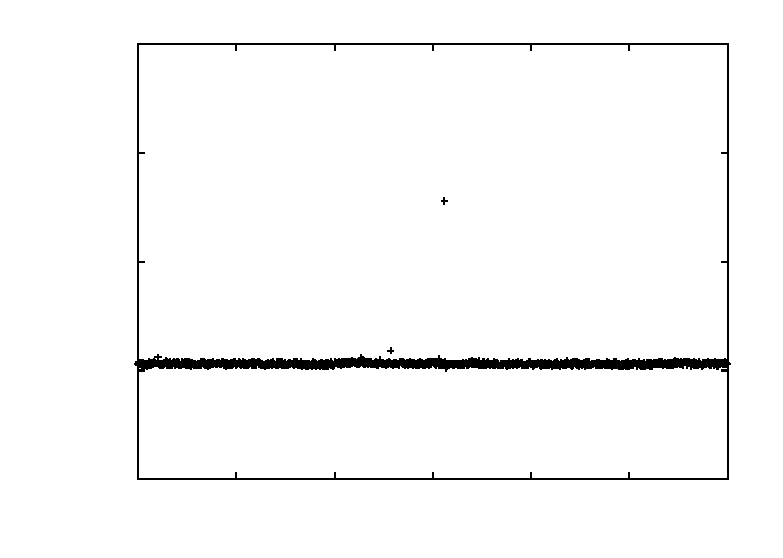
\includegraphics{fig/preSemSchedND}}%
    \gplfronttext
  \end{picture}%
\endgroup
}}}
  \subfloat[\textbf{Linux$^{\mathbf{Prt}}$ - Com carga} \newline
  \vskip 1mm VM:     8.0, DP:     2.0,  Min:     5.2, Max:    31.0]{%
    \label{fig:preTotSchedND}%
    {\scalebox{0.58}{% GNUPLOT: LaTeX picture with Postscript
\begingroup
  \makeatletter
  \providecommand\color[2][]{%
    \GenericError{(gnuplot) \space\space\space\@spaces}{%
      Package color not loaded in conjunction with
      terminal option `colourtext'%
    }{See the gnuplot documentation for explanation.%
    }{Either use 'blacktext' in gnuplot or load the package
      color.sty in LaTeX.}%
    \renewcommand\color[2][]{}%
  }%
  \providecommand\includegraphics[2][]{%
    \GenericError{(gnuplot) \space\space\space\@spaces}{%
      Package graphicx or graphics not loaded%
    }{See the gnuplot documentation for explanation.%
    }{The gnuplot epslatex terminal needs graphicx.sty or graphics.sty.}%
    \renewcommand\includegraphics[2][]{}%
  }%
  \providecommand\rotatebox[2]{#2}%
  \@ifundefined{ifGPcolor}{%
    \newif\ifGPcolor
    \GPcolorfalse
  }{}%
  \@ifundefined{ifGPblacktext}{%
    \newif\ifGPblacktext
    \GPblacktextfalse
  }{}%
  % define a \g@addto@macro without @ in the name:
  \let\gplgaddtomacro\g@addto@macro
  % define empty templates for all commands taking text:
  \gdef\gplbacktext{}%
  \gdef\gplfronttext{}%
  \makeatother
  \ifGPblacktext
    % no textcolor at all
    \def\colorrgb#1{}%
    \def\colorgray#1{}%
  \else
    % gray or color?
    \ifGPcolor
      \def\colorrgb#1{\color[rgb]{#1}}%
      \def\colorgray#1{\color[gray]{#1}}%
      \expandafter\def\csname LTw\endcsname{\color{white}}%
      \expandafter\def\csname LTb\endcsname{\color{black}}%
      \expandafter\def\csname LTa\endcsname{\color{black}}%
      \expandafter\def\csname LT0\endcsname{\color[rgb]{1,0,0}}%
      \expandafter\def\csname LT1\endcsname{\color[rgb]{0,1,0}}%
      \expandafter\def\csname LT2\endcsname{\color[rgb]{0,0,1}}%
      \expandafter\def\csname LT3\endcsname{\color[rgb]{1,0,1}}%
      \expandafter\def\csname LT4\endcsname{\color[rgb]{0,1,1}}%
      \expandafter\def\csname LT5\endcsname{\color[rgb]{1,1,0}}%
      \expandafter\def\csname LT6\endcsname{\color[rgb]{0,0,0}}%
      \expandafter\def\csname LT7\endcsname{\color[rgb]{1,0.3,0}}%
      \expandafter\def\csname LT8\endcsname{\color[rgb]{0.5,0.5,0.5}}%
    \else
      % gray
      \def\colorrgb#1{\color{black}}%
      \def\colorgray#1{\color[gray]{#1}}%
      \expandafter\def\csname LTw\endcsname{\color{white}}%
      \expandafter\def\csname LTb\endcsname{\color{black}}%
      \expandafter\def\csname LTa\endcsname{\color{black}}%
      \expandafter\def\csname LT0\endcsname{\color{black}}%
      \expandafter\def\csname LT1\endcsname{\color{black}}%
      \expandafter\def\csname LT2\endcsname{\color{black}}%
      \expandafter\def\csname LT3\endcsname{\color{black}}%
      \expandafter\def\csname LT4\endcsname{\color{black}}%
      \expandafter\def\csname LT5\endcsname{\color{black}}%
      \expandafter\def\csname LT6\endcsname{\color{black}}%
      \expandafter\def\csname LT7\endcsname{\color{black}}%
      \expandafter\def\csname LT8\endcsname{\color{black}}%
    \fi
  \fi
  \setlength{\unitlength}{0.0500bp}%
  \begin{picture}(7200.00,5040.00)%
    \gplgaddtomacro\gplbacktext{%
      \csname LTb\endcsname%
      \put(1034,594){\makebox(0,0)[r]{\strut{}$0.0$}}%
      \put(1034,1430){\makebox(0,0)[r]{\strut{}$10.0$}}%
      \put(1034,2267){\makebox(0,0)[r]{\strut{}$20.0$}}%
      \put(1034,3103){\makebox(0,0)[r]{\strut{}$30.0$}}%
      \put(1034,3940){\makebox(0,0)[r]{\strut{}$40.0$}}%
      \put(1034,4776){\makebox(0,0)[r]{\strut{}$50.0$}}%
      \put(1166,374){\makebox(0,0){\strut{}$ 0$}}%
      \put(2109,374){\makebox(0,0){\strut{}$ 10$}}%
      \put(3053,374){\makebox(0,0){\strut{}$ 20$}}%
      \put(3996,374){\makebox(0,0){\strut{}$ 30$}}%
      \put(4939,374){\makebox(0,0){\strut{}$ 40$}}%
      \put(5883,374){\makebox(0,0){\strut{}$ 50$}}%
      \put(6826,374){\makebox(0,0){\strut{}$ 60$}}%
      \put(396,2685){\rotatebox{90}{\makebox(0,0){\strut{}Latency ($\mu s$)}}}%
      \put(3996,110){\makebox(0,0){\strut{}Time ($s$)}}%
    }%
    \gplgaddtomacro\gplfronttext{%
    }%
    \gplbacktext
    \put(0,0){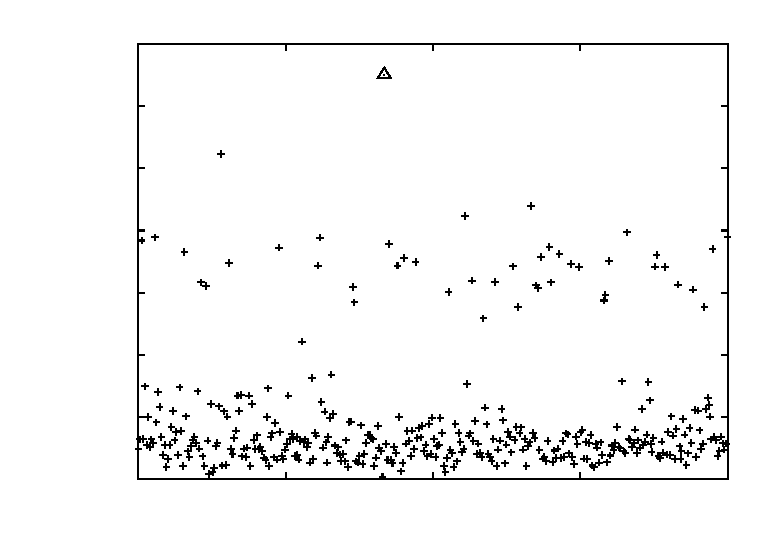
\includegraphics{fig/preTotSchedND}}%
    \gplfronttext
  \end{picture}%
\endgroup
}}}

  \caption[]{Lat�ncia de ativa��o do Linux$^{\mathbf{Prt}}$
    desabilitando o \ing{thread} associado as interrup��es da
    PP (op��o \cod{IRQF\_NODELAY}).}
  \label{fig:latAtivND}%
\end{figure}


\section{Conclus�o}
\label{sec:concPlat}

Neste cap�tulo, os conceitos de sistemas operacionais de prop�sito geral e de
sistemas operacional de tempo real foram apresentados, assim como as principais
abstra��es que s�o necess�rias para a descri��o das suas funcionalidades.  Em
seguida, as principais causas de imprevisibilidade de um SOPG tal como Linux foram
identificadas.

Para descrever os desafios que devem ser resolvidos para tornar um
SOPG mais previs�vel, tr�s solu��es baseadas em Linux foram descritas
em detalhes. Experimentos foram realizados com o objetivo de comparar as
tr�s solu��es de SOTR baseadas em Linux consideradas para a
implementa��o de \doris.

A metodologia experimental permitiu medir as
lat�ncias de interrup��o e de ativa��o, em situa��es de carga
vari�vel, tanto do processador quanto de eventos externos tratados por
interrup��o.  Linux padr�o apresentou lat�ncias no pior caso acima de
$100\mu s$, enquanto as plataformas Linux$^{\mathbf{Prt}}$,
Linux$^{\mathbf{Rtai}}$ e Linux$^{\mathbf{Xen}}$ conseguiram prover
garantias temporais com uma precis�o abaixo de $20\mu s$. No entanto,
para se conseguir este comportamento em rela��o ao
Linux$^{\mathbf{Prt}}$, foi necess�rio desabilitar \ing{threads} de
interrup��o, tornando o sistema menos flex�vel. Com tais
\ing{threads}, o comportamento de Linux$^{\mathbf{Prt}}$ sofreu
consider�vel degrada��o da sua previsibilidade temporal. 

Observa-se que os experimentos foram realizados numa arquitetura espec�fica e que
resultados quantitativamente diferentes teriam provavelmente sido encontradas em
outras configura��es de m�quinas. No entanto, os resultados obtidos aqui s�o
qualitativamente consistentes com os resultados apresentados em trabalhos similares
\cite{Rostedt07, Siro07, Benoit05, Dozio03}.

Mais especificamente, o presente trabalho apresentou resultados de lat�ncia de
interrup��o que confirmam os resultados obtidos em \cite{Benoit05},
numa avalia��o bastante abrangente do \ing{patch} Adeos, publicada
apenas na Internet. J� os resultados encontrados aqui para
Linux$^{\mathbf{Prt}}$, sem a op��o \cod{IRQF\_NODELAY}, diferiram dos
apresentados por \cite{Benoit05}, pois uma degrada��o das garantias
temporais por esta plataforma foi observada, tal como visto na se��o
\ref{sec:latIrq}. Em rela��o �s lat�ncias de ativa��o, n�o temos
conhecimento de nenhum outro trabalho comparativo.

A proposta do projeto Xenomai se destacou pelo fato de oferecer um ambiente de
programa��o em modo usu�rio e ao mesmo tempo conseguir tempos de lat�ncia
t�picos das solu��es baseadas em \nanokernel.



%%
%% Parte p�s-textual
%%
\backmatter

\renewcommand{\bibname}{REFER�NCIAS}
%\nocite{*}
%\bibliographystyle{authordate2}
%\bibliographystyle{abnt-alf}

\bibliography{/home/paul/texmf/bib}

%% Fim do documento
\end{document}
